\documentclass[UTF8,a4paper,11pt]{ctexart}

\usepackage[margin=1in]{geometry}
\usepackage{amsmath, amssymb}
\usepackage{booktabs}
\usepackage{array}
\usepackage{tabularx}
\usepackage{graphicx}
\usepackage{caption}
\usepackage{subcaption}
\usepackage{float}
\usepackage{hyperref}
\usepackage{xcolor}
\usepackage{enumitem}
\usepackage{setspace}
\usepackage{pgfplots}

\pgfplotsset{compat=1.18}
\captionsetup{font=small, labelfont=bf}
\hypersetup{hidelinks}
\setlist[itemize]{leftmargin=2.0em, itemsep=0.25em, topsep=0.3em}
\setlist[enumerate]{leftmargin=2.2em, itemsep=0.25em, topsep=0.3em}
\setlength{\parindent}{2em}
\setlength{\parskip}{0.2em}
\setstretch{1.16}
\renewcommand{\arraystretch}{1.16}

\newcommand{\accpm}[2]{#1\% $\pm$ #2 个百分点}
\newcommand{\code}[1]{\texttt{#1}}

\begin{document}

\begin{center}
    {\zihao{1}\bfseries Homework 2\par}
    \vspace{0.5em}
    {\zihao{3}\bfseries 深度学习与空间智能\par}
    \vspace{1.0em}
    {\zihao{2}\bfseries 基于深度神经网络的视觉识别实验报告\par}
    \vspace{0.4em}
    {\zihao{3}\bfseries 花卉图像分类、道路车辆检测与语义分割\par}
\end{center}

\vspace{0.6em}

\begin{center}
    \small
    \begin{tabular}{lll}
        \toprule
        成员 & 学号 & 主要分工 \\
        \midrule
        朱宇玄 & 25110980033 & 花卉图像分类实验 \\
        钱玲萱 & 24110980018 & 道路车辆检测与跟踪实验 \\
        吉张林 & 25110980010 & 语义分割实验 \\
        \bottomrule
    \end{tabular}
\end{center}

\vspace{0.4em}

\begin{center}
    \small
    GitHub 项目地址：待补充 \qquad 模型权重网盘地址：待补充
\end{center}

\vspace{0.6em}

\begin{abstract}
本文围绕三类典型视觉识别问题展开实验：细粒度花卉图像分类、道路车辆检测与跟踪、场景语义分割。花卉分类实验使用 Oxford 102 Flowers 数据集，系统比较 ResNet baseline、ImageNet 预训练与从零训练、SE/CBAM 注意力模块、ViT/Swin Transformer 以及 ConvNeXt 等现代卷积网络；最终 ConvNeXt-Tiny 在 384px 输入和 10 个随机种子下取得 \accpm{95.60}{0.61} 的测试准确率。车辆检测实验使用 YOLOv8s 在道路车辆数据集上训练检测器，验证集 mAP50 为 0.520，并结合 ByteTrack 完成跟踪 ID 显示、越线计数和遮挡失败分析。语义分割实验从零实现轻量 U-Net，在 Stanford Background / ICCV09 风格数据上比较 Cross-Entropy、Dice 与组合损失，Dice Loss 取得最高验证集 mIoU 0.3055。实验结果表明，预训练特征、注意力机制、输入分辨率、检测稳定性和区域重叠损失都会显著影响视觉识别系统的最终泛化性能。
\end{abstract}

\section{引言}

深度学习视觉系统通常可以分为图像级识别、目标级检测跟踪和像素级语义理解三个层次。图像分类关注整张图片属于哪个类别；目标检测需要在图像或视频中定位多个实例；语义分割则要求对每个像素进行类别判定。三类问题对应不同的监督信号、模型结构和评价指标，也体现了深度神经网络在空间智能问题中的不同建模方式。

本文实验分为三个部分。第一部分研究 Oxford 102 Flowers 细粒度图像分类，该数据集每类训练样本很少，适合分析 ImageNet 预训练、注意力模块和现代 backbone 对小样本分类的影响。第二部分研究道路车辆检测与跟踪，重点是 YOLOv8 检测器、ByteTrack 轨迹维持和遮挡场景下的 ID 跳变。第三部分研究语义分割，使用手写 U-Net 比较不同损失函数对 mIoU 的影响。

本文的写作重点放在实验方法、训练设置、定量结果和结果分析上。所有表格中的 accuracy 均为百分比；检测结果使用 precision、recall 和 mAP；分割结果使用 pixel accuracy 和 mIoU。

\section{花卉图像分类实验}

\subsection{数据集与预处理}

花卉分类实验使用 Oxford 102 Category Flower Dataset。数据集共包含 8189 张花卉图像，类别数为 102。每个类别对应一种花卉，图像具有明显的细粒度分类特征：不同类别之间常常只在花瓣形状、颜色组合、花蕊结构、局部纹理或拍摄角度上存在差异。因此，该问题比普通粗粒度图像分类更依赖高质量特征表示。

实验中严格使用数据集官方划分文件。其中 \code{setid.mat} 保存训练集、验证集和测试集的图像编号，\code{imagelabels.mat} 保存每张图片的类别标签。读取标签时，代码将 MATLAB 中从 1 开始的类别编号转换为 PyTorch 中从 0 开始的类别编号。

\begin{table}[H]
    \centering
    \caption{Oxford 102 Flowers 官方数据划分}
    \small
    \begin{tabular}{lrrl}
        \toprule
        数据子集 & 样本数 & 类别数 & 用途 \\
        \midrule
        训练集 & 1020 & 102 & 参数学习与数据增强 \\
        验证集 & 1020 & 102 & 模型选择与 early stopping \\
        测试集 & 6149 & 102 & 最终泛化性能评估 \\
        \bottomrule
    \end{tabular}
\end{table}

图 \ref{fig:classification-dataset-samples} 给出了数据集中不同类别的代表性样例。可以看到，不同花卉类别之间往往只在颜色分布、花瓣形状、局部纹理和拍摄视角上存在细微差异；同时每类训练图像只有 10 张，这也是后续预训练和数据增强对结果影响明显的原因。

\begin{figure}[H]
    \centering
    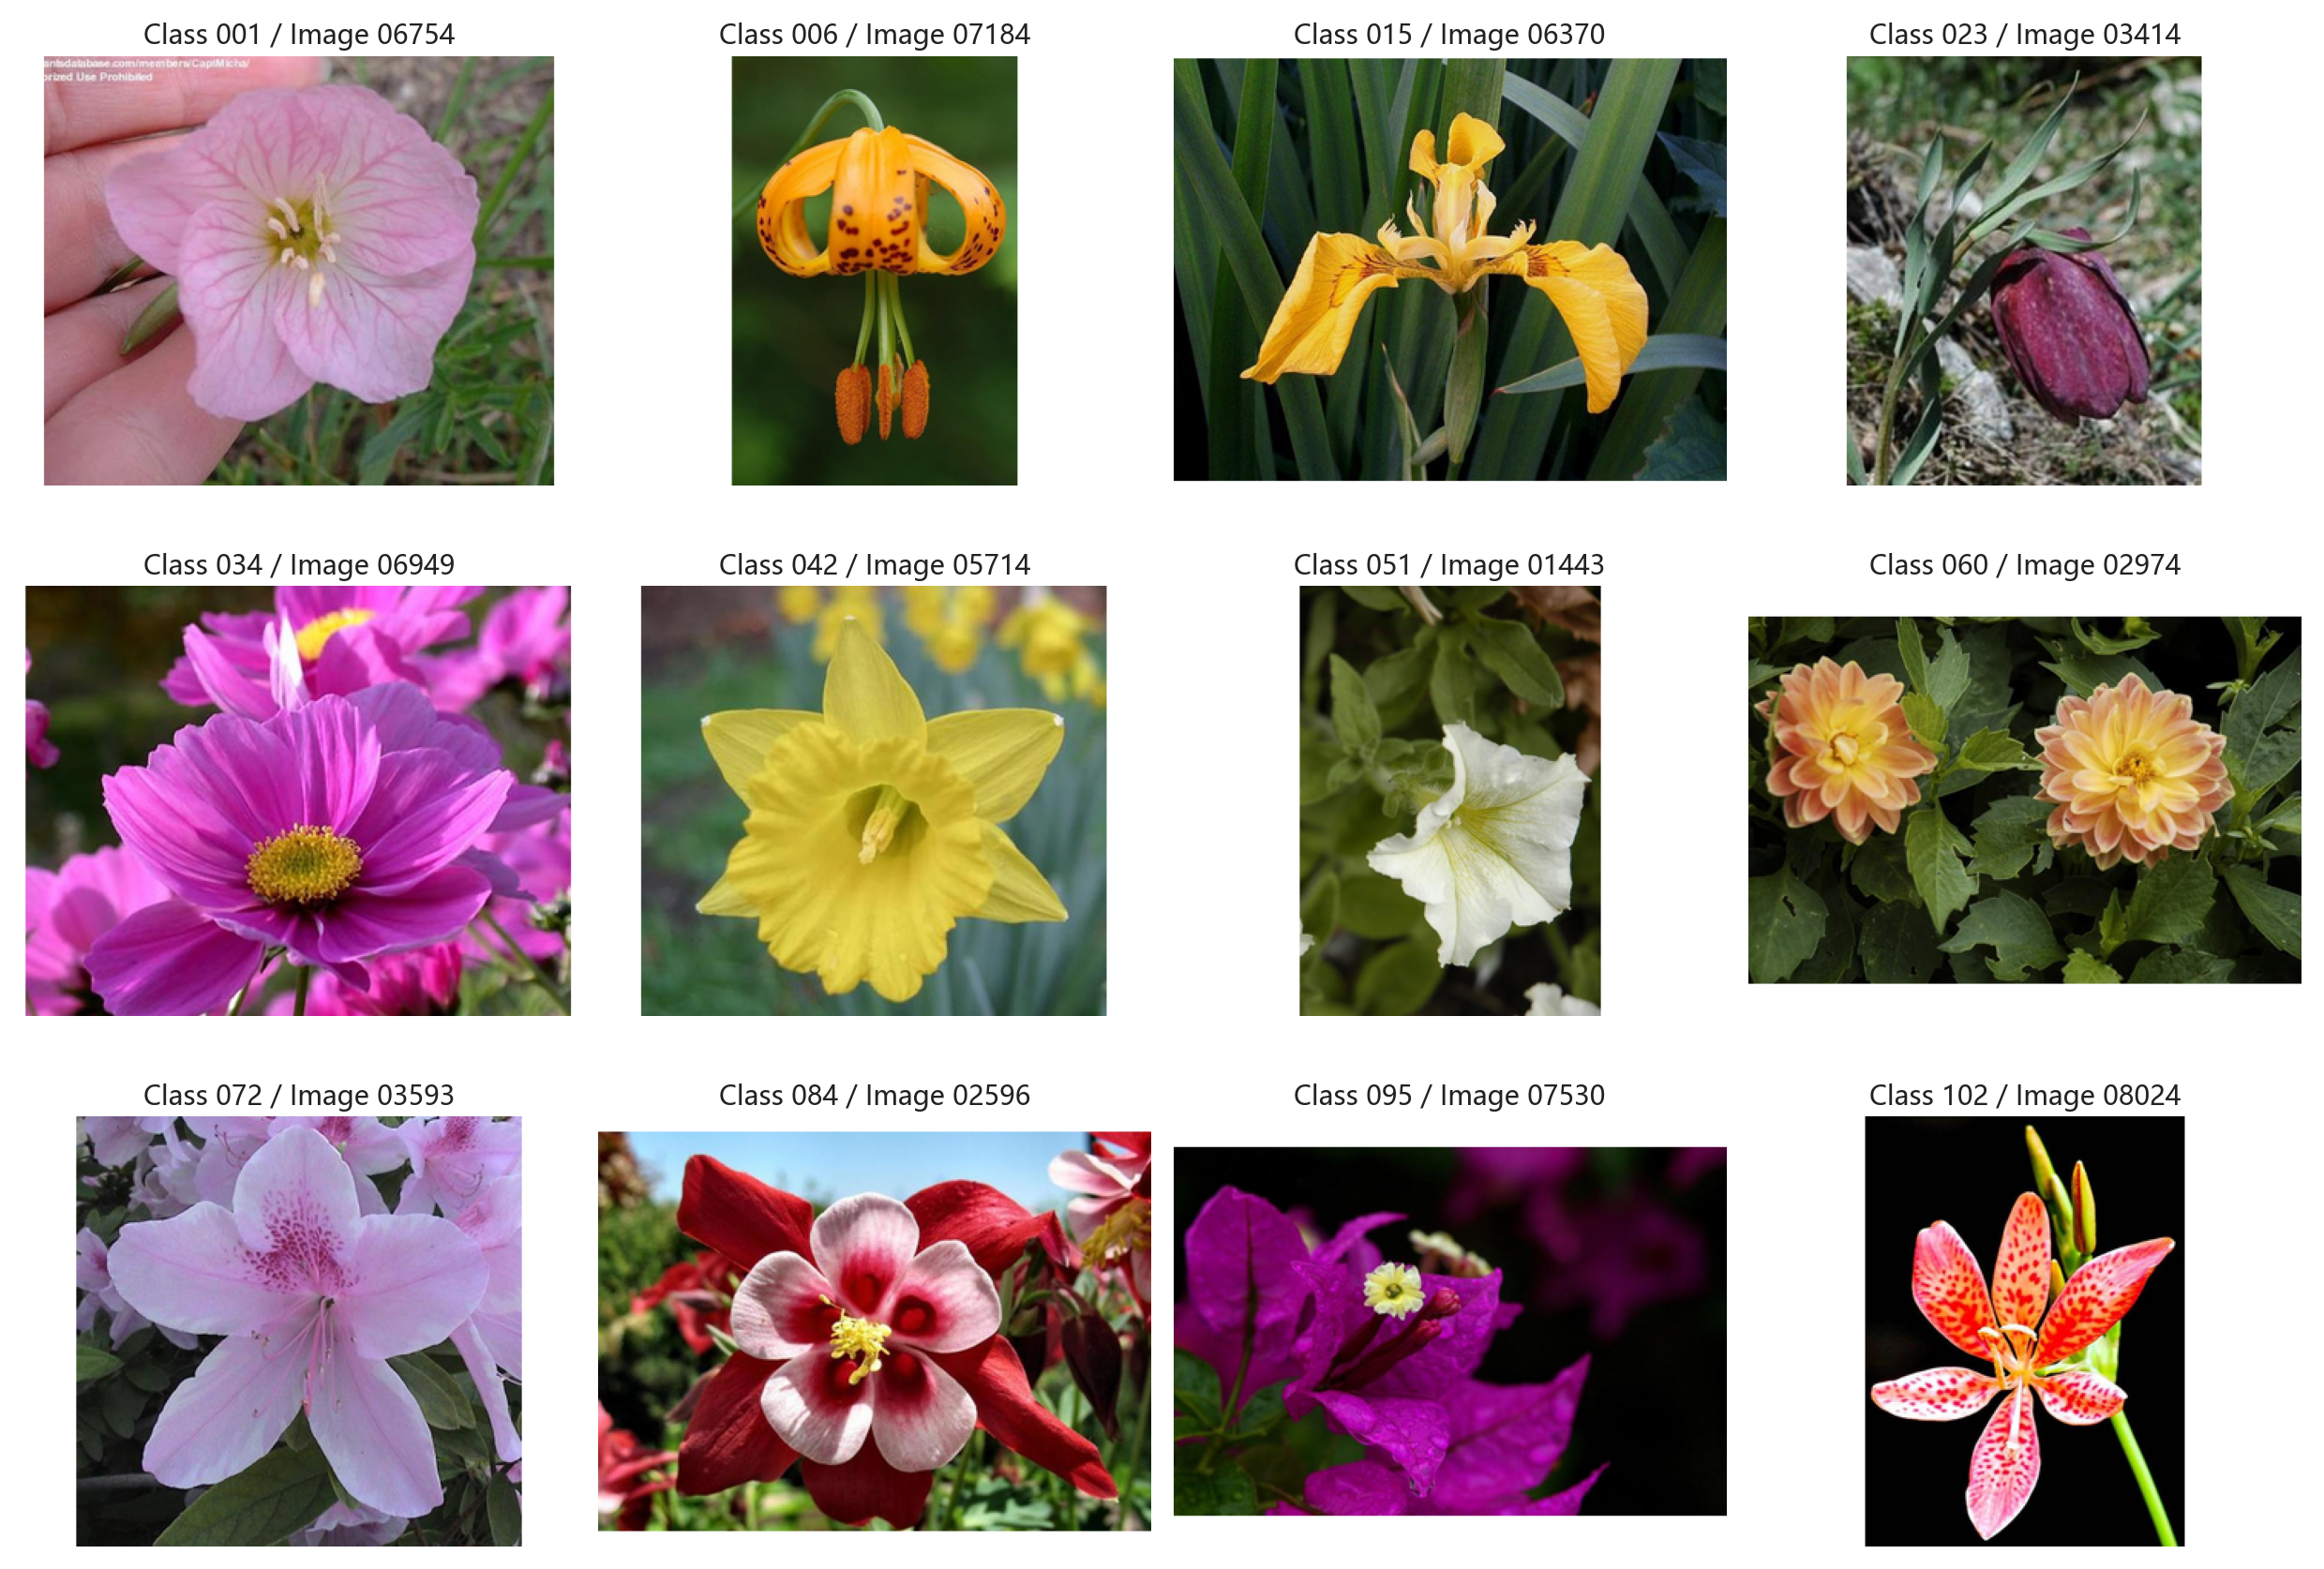
\includegraphics[width=0.90\textwidth]{../tasks/task1_flower_classification/experiment_results/final_report/figures/task1_dataset_samples.png}
    \caption{Oxford 102 Flowers 数据集样例}
    \label{fig:classification-dataset-samples}
\end{figure}

为了适配 torchvision 中的 ResNet、ConvNeXt、ViT 和 Swin 模型，基础实验使用 224$\times$224 输入尺寸；后续进一步补充了 ConvNeXt-Tiny 384px 输入实验。训练阶段采用随机裁剪和颜色扰动以缓解小训练集带来的过拟合，验证和测试阶段则使用确定性的 resize 与 center crop，保证模型选择和最终测试结果稳定可复现。

\begin{itemize}
    \item 训练集：\code{RandomResizedCrop(image\_size, scale=(0.7, 1.0))}、随机水平翻转、亮度/对比度/饱和度扰动；
    \item 验证集和测试集：先 resize 到约 \(1.14 \times\) 目标尺寸，再进行 center crop；
    \item 归一化：使用 ImageNet 均值 (0.485, 0.456, 0.406) 与标准差 (0.229, 0.224, 0.225)；
    \item 损失函数：使用 CrossEntropyLoss，并在主要实验中加入 label smoothing。
\end{itemize}

\subsection{模型结构}

\subsubsection*{ResNet baseline}

Baseline 使用 ResNet-18 和 ResNet-34。对于 ImageNet 预训练实验，模型主体加载 torchvision 中的 ImageNet-1K 预训练权重，仅将最后的全连接分类层替换为 102 类输出：

\begin{equation}
    z = f_{\theta}(x), \qquad p = \mathrm{softmax}(Wz + b), \qquad p \in \mathbb{R}^{102}.
\end{equation}

从零训练实验使用相同结构，但不加载 ImageNet 权重，全部参数随机初始化后在 Oxford 102 数据集上训练。由于训练集仅 1020 张图像，从零训练的模型更容易受到样本规模限制，实验结果也可用于衡量预训练对小样本细粒度分类的贡献。

\subsubsection*{SE 与 CBAM 注意力模块}

在 CNN 注意力实验中，本文分别构建了 ResNet-18-SE、ResNet-34-SE、ResNet-18-CBAM 与 ResNet-34-CBAM。实现方式是在 ResNet 的 layer4 后加入注意力模块，使模型在高层语义特征上重新分配通道或空间权重。

SE-block 通过全局平均池化得到通道描述，再使用两层 \(1 \times 1\) 卷积完成压缩与激励：

\begin{equation}
    s = \sigma(W_2 \delta(W_1 \mathrm{GAP}(F))), \qquad F_e = F \odot s.
\end{equation}

CBAM 在 SE 式通道注意力之外进一步加入空间注意力。通道注意力使用平均池化与最大池化两条分支，空间注意力则在通道维度上计算 average map 和 max map 后使用 \(7 \times 7\) 卷积生成空间权重。这样模型不仅能判断“哪些通道更重要”，也能判断“图像中哪些区域更重要”。

\subsubsection*{Transformer 与现代卷积网络}

除 CNN baseline 和注意力模型外，本实验还训练了 ViT-B/16 与 Swin-T。ViT-B/16 将图像切分为 patch 后通过自注意力建模全局关系；Swin-T 则使用 shifted window attention，在局部窗口内计算注意力并通过窗口移动实现跨窗口信息交换。二者均使用 ImageNet 预训练权重，并将最后分类头替换为 102 类输出。

现代卷积网络实验补充了 ResNet-50、ResNet-101、EfficientNet-B0、EfficientNet-B3 和 ConvNeXt-Tiny。补充这些模型的目的是检查在 Swin-T 之外，现代 CNN 架构是否能在小样本细粒度分类中提供更稳定的泛化能力。最终结果表明，ConvNeXt-Tiny 配合 384px 输入取得了最高且更稳定的多随机种子平均测试准确率。

\subsection{实验设置}

正式实验在 GPU 环境中完成。训练过程中每个 epoch 都记录训练集 loss、训练集 accuracy、验证集 loss、验证集 accuracy 和当前学习率。每当验证集 accuracy 刷新最高值时保存 checkpoint；若连续若干个 epoch 未提升，则 early stopping。最终测试时加载验证集表现最好的 checkpoint，而不是最后一个 epoch 的参数。

\begin{table}[H]
    \centering
    \caption{花卉分类训练策略}
    \small
    \begin{tabular}{ll}
        \toprule
        项目 & 设置 \\
        \midrule
        优化器 & AdamW \\
        学习率调度 & CosineAnnealingLR \\
        最大 epoch & 200 \\
        Early stopping & 监控验证集 accuracy \\
        损失函数 & CrossEntropyLoss，可选 label smoothing \\
        评价指标 & validation accuracy 与 test accuracy \\
        模型选择 & 保存验证集 accuracy 最优 checkpoint \\
        \bottomrule
    \end{tabular}
\end{table}

基础网格包含 CNN 与 Transformer 两部分。CNN 网格包含 baseline、SE、CBAM 和从零训练模型；Transformer 网格包含 ViT-B/16 与 Swin-T。完整搜索空间如表 \ref{tab:classification-search-space} 所示。

\begin{table}[H]
    \centering
    \caption{花卉分类基础超参数搜索空间}
    \label{tab:classification-search-space}
    \small
    \resizebox{\textwidth}{!}{%
    \begin{tabular}{llllll}
        \toprule
        组别 & 模型 & 设置 & 学习率 & Batch size & Label smoothing \\
        \midrule
        CNN & ResNet-18 & baseline & \(1\times10^{-3}, 3\times10^{-4}\) & 32, 64 & 0, 0.1 \\
        CNN & ResNet-34 & baseline & \(1\times10^{-3}, 3\times10^{-4}\) & 32, 64 & 0, 0.1 \\
        CNN & ResNet-18 & SE 模块 & \(1\times10^{-3}, 3\times10^{-4}\) & 32, 64 & 0, 0.1 \\
        CNN & ResNet-34 & SE 模块 & \(1\times10^{-3}, 3\times10^{-4}\) & 32, 64 & 0, 0.1 \\
        CNN & ResNet-18 & CBAM & \(1\times10^{-3}, 3\times10^{-4}\) & 32, 64 & 0, 0.1 \\
        CNN & ResNet-34 & CBAM & \(1\times10^{-3}, 3\times10^{-4}\) & 32, 64 & 0, 0.1 \\
        CNN & ResNet-18 & 从零训练 & \(1\times10^{-3}, 3\times10^{-4}\) & 32, 64 & 0, 0.1 \\
        CNN & ResNet-34 & 从零训练 & \(1\times10^{-3}, 3\times10^{-4}\) & 32, 64 & 0, 0.1 \\
        Transformer & ViT-B/16 & 预训练 & \(3\times10^{-4}, 1\times10^{-4}\) & 16, 32 & 0, 0.1 \\
        Transformer & Swin-T & 预训练 & \(3\times10^{-4}, 1\times10^{-4}\) & 16, 32 & 0, 0.1 \\
        \bottomrule
    \end{tabular}%
    }
\end{table}

CNN 网格中 weight decay 取 \(1\times10^{-4}\) 和 \(1\times10^{-5}\)；Transformer 网格中 weight decay 固定为 \(1\times10^{-4}\)。在基础网格基础上，后续继续进行了扩展 CNN、随机种子重复、ConvNeXt 最终检查、384px 分辨率扩展和小规模调参。最终花卉分类部分共纳入 303 次训练结果用于比较分析。

\begin{table}[H]
    \centering
    \caption{花卉分类模型比较范围}
    \small
    \begin{tabular}{lr}
        \toprule
        比较组别 & 训练次数 \\
        \midrule
        CNN baseline、SE/CBAM 与 scratch/pretrained 网格 & 128 \\
        ViT-B/16 与 Swin-T 网格 & 16 \\
        扩展预训练 CNN 网格 & 120 \\
        扩展 CNN 随机种子重复 & 3 \\
        补充重复实验 & 12 \\
        ConvNeXt 最终检查 & 10 \\
        ConvNeXt 384px 分辨率扩展 & 14 \\
        \midrule
        合计 & 303 \\
        \bottomrule
    \end{tabular}
\end{table}

\subsection{总体分类结果}

基础网格中，Swin-T 取得最高测试准确率 94.26\%，最优 CNN 模型为 ResNet-34-CBAM，测试准确率为 92.15\%。从零训练的 ResNet-34 虽然优于从零训练的 ResNet-18，但测试准确率只有 55.44\%，与预训练模型存在非常明显的差距。

\begin{table}[H]
    \centering
    \caption{基础网格中各模型/训练模式的最优结果}
    \small
    \begin{tabular}{llrrrr}
        \toprule
        模型 & 设置 & 预训练 & Batch size & Val Acc. & Test Acc. \\
        \midrule
        Swin-T & Transformer & 是 & 16 & 95.98\% & 94.26\% \\
        ViT-B/16 & Transformer & 是 & 32 & 95.00\% & 92.83\% \\
        ResNet-18 & CBAM & 是 & 64 & 94.12\% & 90.86\% \\
        ResNet-34 & CBAM & 是 & 64 & 93.92\% & 92.15\% \\
        ResNet-18 & SE-block & 是 & 32 & 93.63\% & 90.65\% \\
        ResNet-34 & SE-block & 是 & 32 & 93.43\% & 89.72\% \\
        ResNet-18 & baseline & 是 & 32 & 92.94\% & 89.97\% \\
        ResNet-34 & baseline & 是 & 64 & 92.65\% & 89.58\% \\
        ResNet-34 & 从零训练 & 否 & 32 & 61.67\% & 55.44\% \\
        ResNet-18 & 从零训练 & 否 & 32 & 59.12\% & 52.72\% \\
        \bottomrule
    \end{tabular}
\end{table}

扩展实验进一步显示，ConvNeXt-Tiny 在该数据集上比单次 Swin-T 最优结果更稳定。最终选择 ConvNeXt-Tiny 384px，学习率 \(1\times10^{-4}\)，weight decay \(1\times10^{-5}\)，batch size 16，label smoothing 0.1。该配置在 10 个随机种子上取得 \accpm{95.60}{0.61} 的测试准确率。

\begin{table}[H]
    \centering
    \caption{扩展模型关键结果对比}
    \small
    \resizebox{\textwidth}{!}{%
    \begin{tabular}{lrrrrrr}
        \toprule
        模型/实验组 & 图像尺寸 & 实验次数 & 学习率 & WD & Val Acc. & Test Acc. \\
        \midrule
        Swin-T 最优单次 & 224 & 1 & 0.0001 & \(10^{-4}\) & 95.98\% & 94.26\% \\
        Swin-T 重复实验 & 224 & 3 & 0.0001 & \(10^{-4}\) & \accpm{96.05}{0.32} & \accpm{93.98}{0.26} \\
        ConvNeXt-Tiny 224px 最优单次 & 224 & 1 & 0.0003 & \(10^{-4}\) & 96.67\% & 94.67\% \\
        ConvNeXt-Tiny 224px 稳定配置 & 224 & 10 & 0.0001 & \(10^{-5}\) & \accpm{96.64}{0.45} & \accpm{94.71}{0.31} \\
        ConvNeXt-Tiny 384px 最终配置 & 384 & 10 & 0.0001 & \(10^{-5}\) & \accpm{97.28}{0.48} & \accpm{95.60}{0.61} \\
        \bottomrule
    \end{tabular}%
    }
\end{table}

\begin{figure}[H]
    \centering
    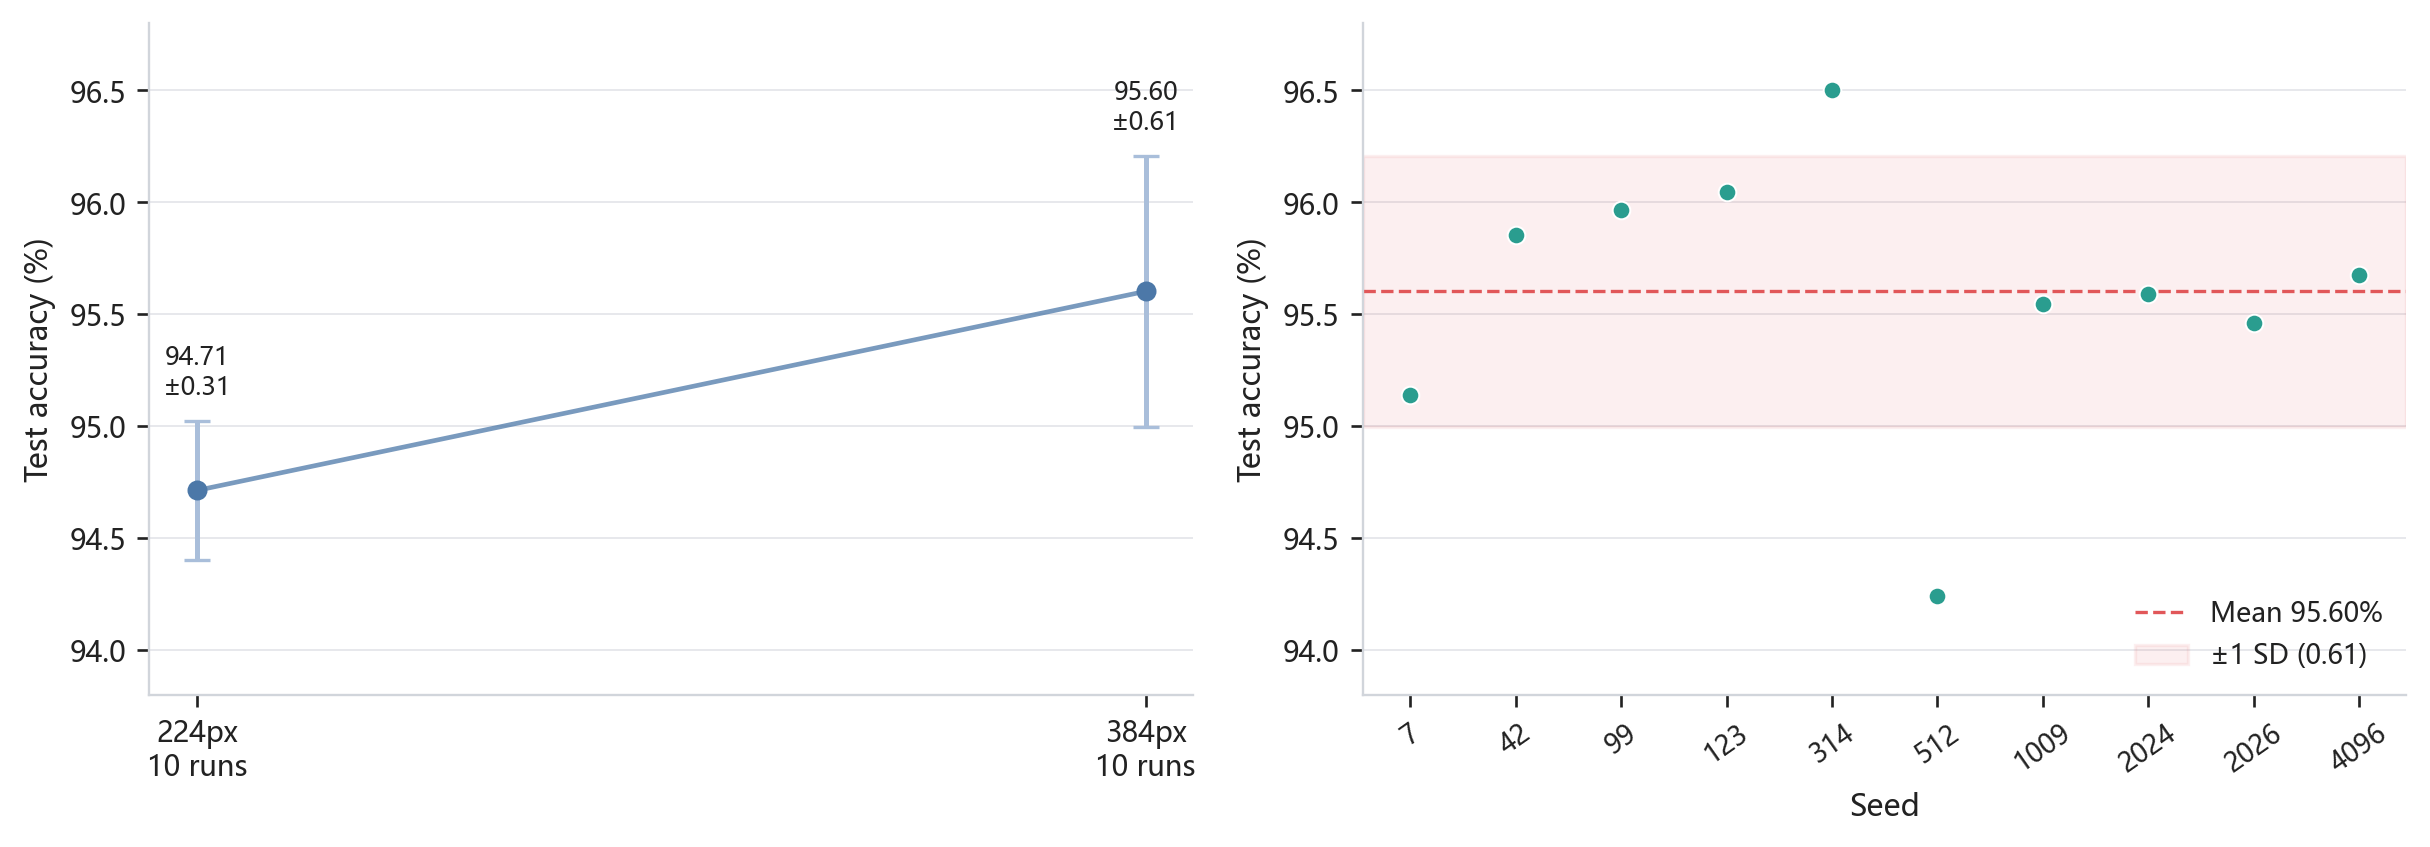
\includegraphics[width=0.86\textwidth]{../tasks/task1_flower_classification/experiment_results/final_report/figures/task1_convnext_resolution_stability.png}
    \caption{ConvNeXt-Tiny 输入分辨率与随机种子稳定性对比}
    \label{fig:classification-convnext-stability}
\end{figure}

\begin{figure}[H]
    \centering
    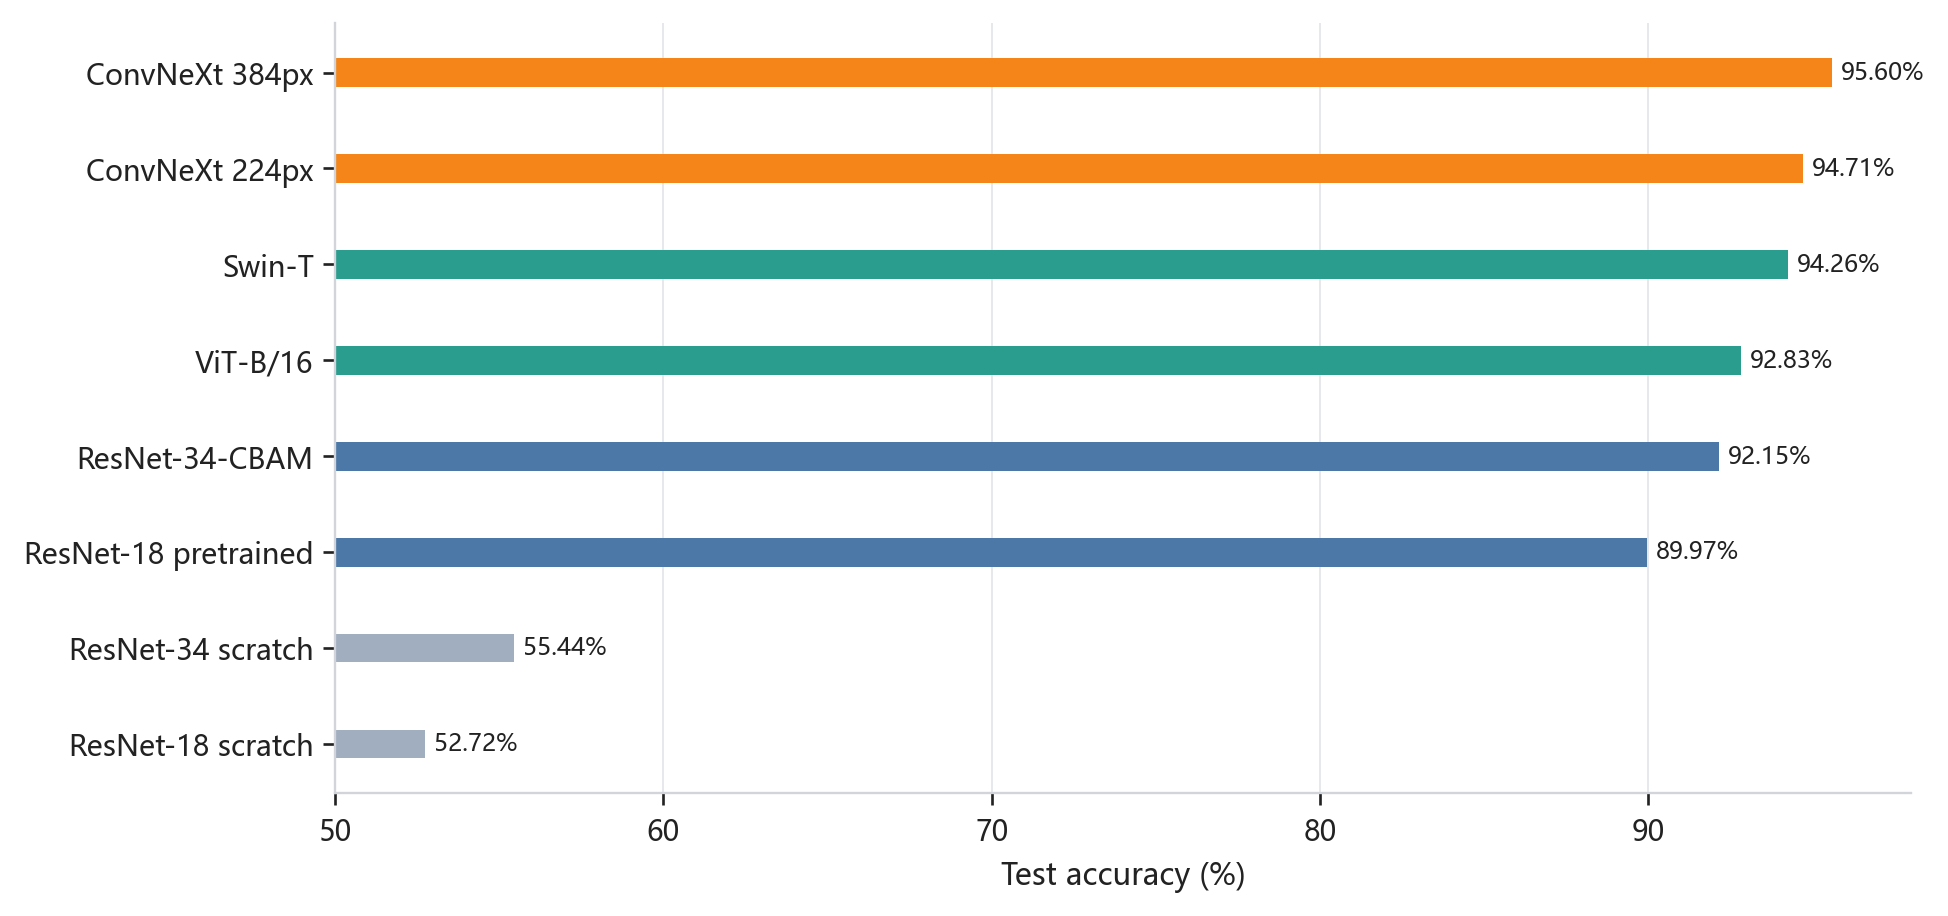
\includegraphics[width=0.86\textwidth]{../tasks/task1_flower_classification/experiment_results/final_report/figures/task1_model_accuracy_comparison.png}
    \caption{不同模型代表性测试准确率对比}
\end{figure}

\subsection{训练过程可视化}

图 \ref{fig:classification-acc-curve} 展示了最终 ConvNeXt-Tiny 384px 配置中一个代表性随机种子的训练过程。该模型在前几个 epoch 内快速收敛，验证集准确率在第 3 个 epoch 已达到 93.43\%，随后逐步提升并在第 31 个 epoch 首次达到最高验证准确率 97.75\%。第 46 个 epoch 触发 early stopping，说明后期继续训练对验证集泛化性能已经没有稳定收益。

\begin{figure}[H]
    \centering
    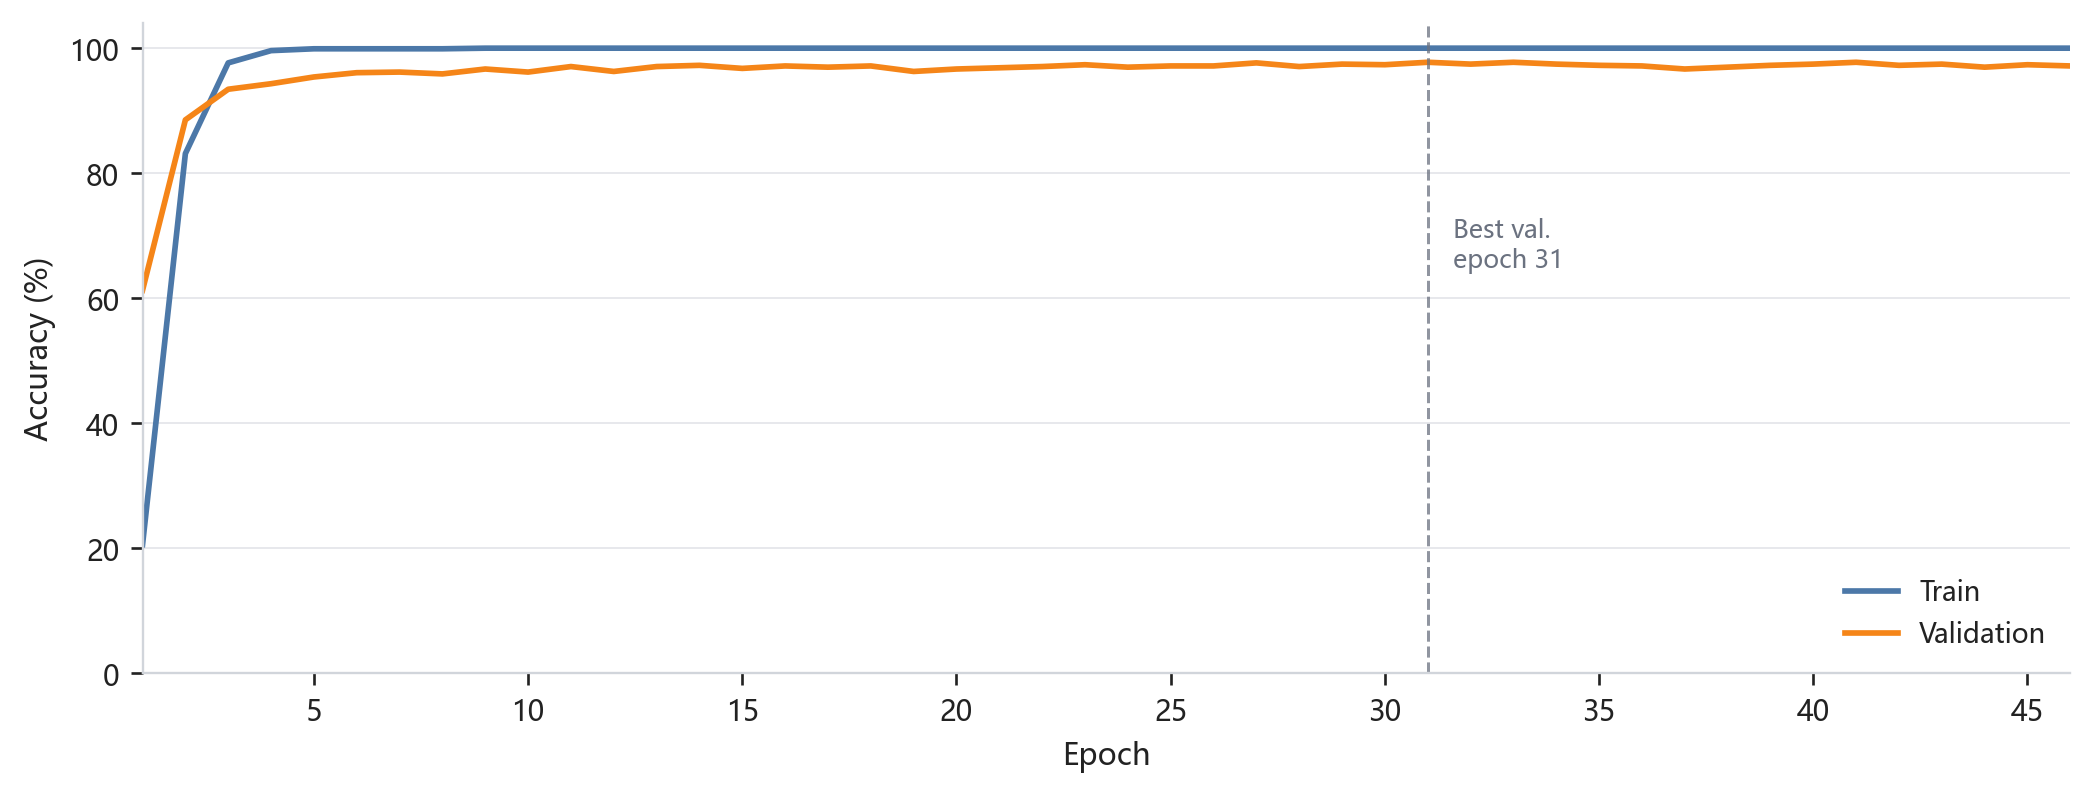
\includegraphics[width=0.86\textwidth]{../tasks/task1_flower_classification/experiment_results/final_report/figures/task1_training_accuracy.png}
    \caption{最终 ConvNeXt-Tiny 384px 模型训练集与验证集准确率曲线}
    \label{fig:classification-acc-curve}
\end{figure}

图 \ref{fig:classification-loss-curve} 给出了同一模型的 loss 曲线。训练 loss 迅速下降并接近稳定，验证 loss 在前期下降明显，后期有小幅波动。这一现象与细粒度小样本分类问题的特点一致：预训练模型可以很快拟合训练集，但验证集性能提升受类别间细微差异、数据增强随机性和训练样本规模共同限制。

\begin{figure}[H]
    \centering
    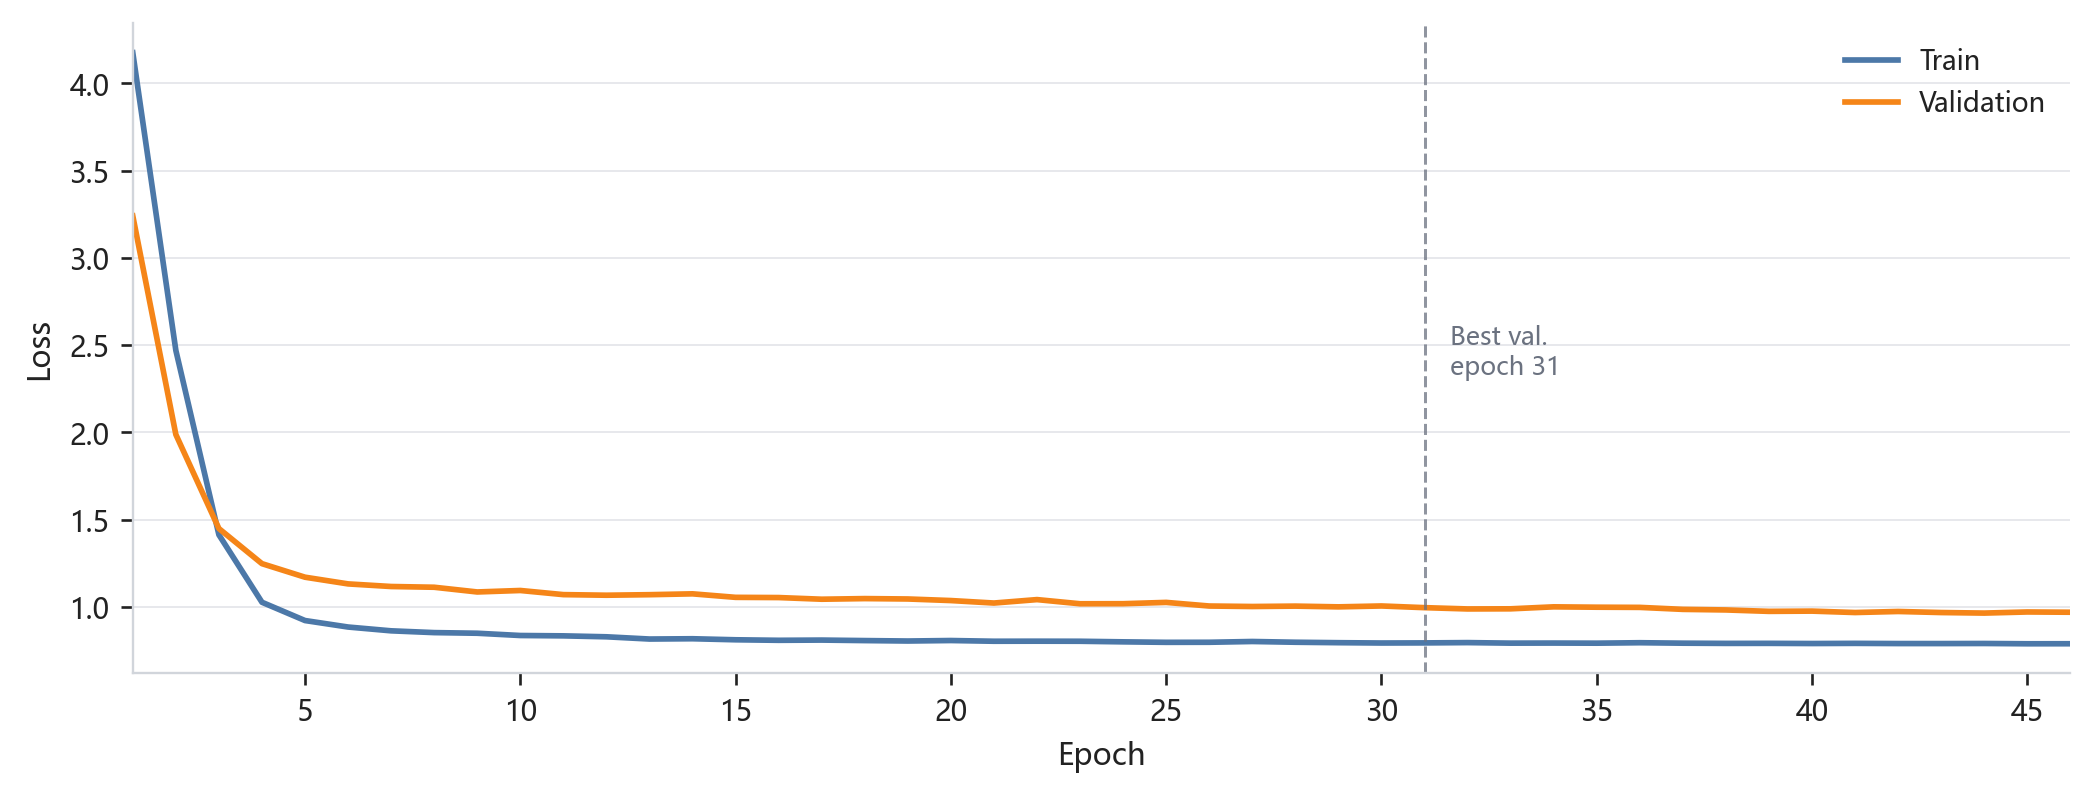
\includegraphics[width=0.86\textwidth]{../tasks/task1_flower_classification/experiment_results/final_report/figures/task1_training_loss.png}
    \caption{最终 ConvNeXt-Tiny 384px 模型训练集与验证集 loss 曲线}
    \label{fig:classification-loss-curve}
\end{figure}

\subsection{预训练消融实验}

预训练消融实验的结论非常明显。采用 ImageNet 权重时，两个 ResNet 的测试准确率接近 90\%；从零训练时仅约 53\%--55\%。具体而言，ResNet-18 从 52.72\% 提升到 89.97\%，ResNet-34 从 55.44\% 提升到 89.58\%。两组差距均超过 34 个百分点。

\begin{table}[H]
    \centering
    \caption{ImageNet 预训练与从零训练的对比}
    \small
    \begin{tabular}{llrrr}
        \toprule
        模型 & 初始化方式 & Best epoch & Val Acc. & Test Acc. \\
        \midrule
        ResNet-18 & ImageNet 预训练 & 42 & 92.94\% & 89.97\% \\
        ResNet-18 & 随机初始化 & 102 & 59.12\% & 52.72\% \\
        ResNet-34 & ImageNet 预训练 & 28 & 92.65\% & 89.58\% \\
        ResNet-34 & 随机初始化 & 96 & 61.67\% & 55.44\% \\
        \bottomrule
    \end{tabular}
\end{table}

\begin{figure}[H]
    \centering
    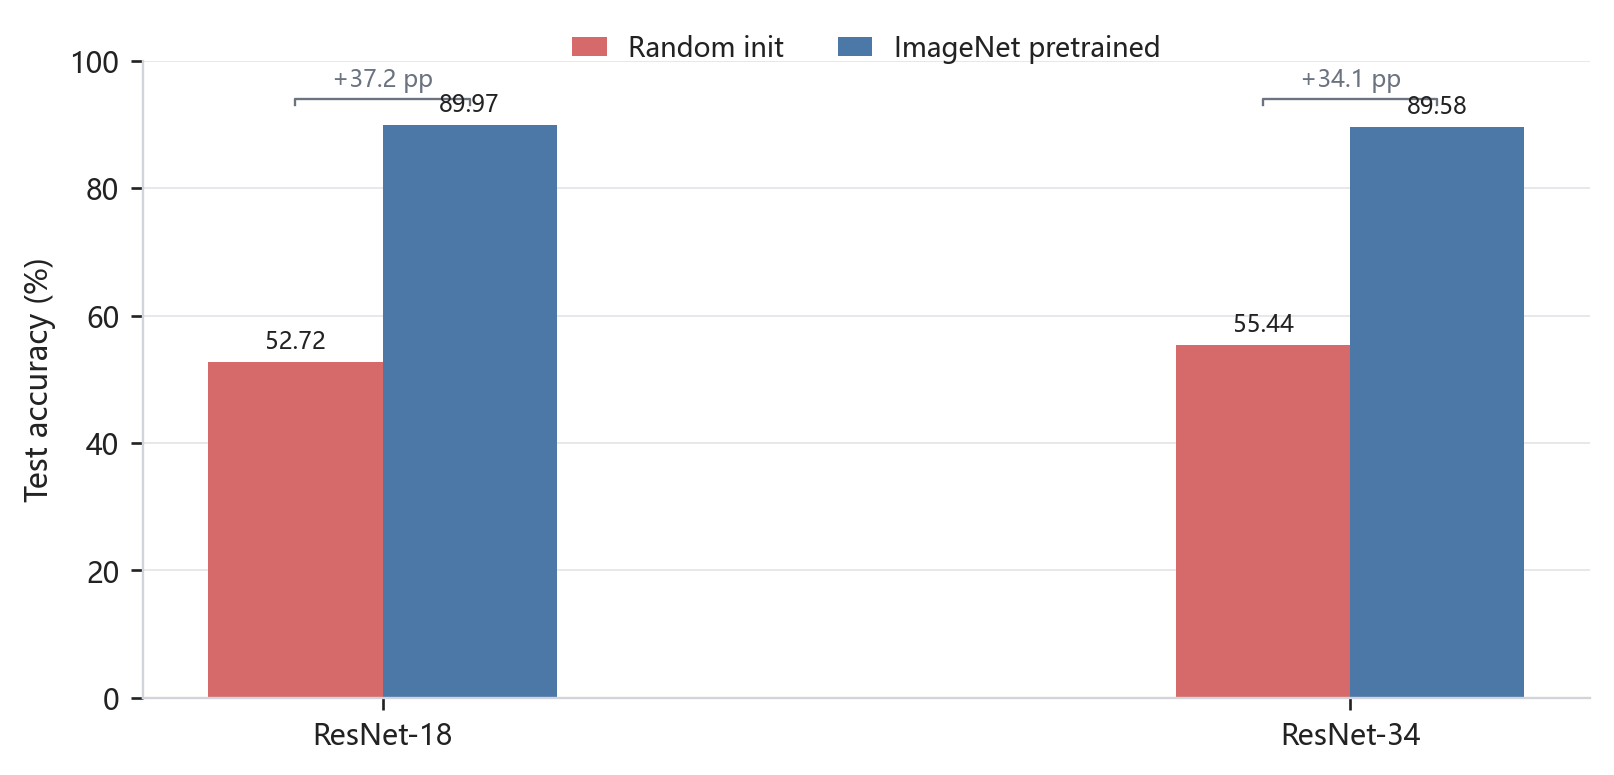
\includegraphics[width=0.68\textwidth]{../tasks/task1_flower_classification/experiment_results/final_report/figures/task1_pretraining_ablation.png}
    \caption{ImageNet 预训练对 ResNet baseline 的提升}
    \label{fig:classification-pretraining-ablation}
\end{figure}

这一结果说明，Oxford 102 的训练集规模不足以让 ResNet 从随机初始化中学习到足够稳健的低层纹理、中层形状和高层语义特征。ImageNet 预训练提供了通用视觉特征，后续微调主要需要适配花卉类别边界，因此收敛速度更快，泛化性能也显著更高。

\subsection{注意力模块分析}

在预训练 ResNet baseline 的基础上加入注意力模块后，整体性能有所提升。ResNet-18 baseline 的测试准确率为 89.97\%，加入 SE 后提升到 90.65\%，加入 CBAM 后提升到 90.86\%。ResNet-34-CBAM 的测试准确率达到 92.15\%，是基础 CNN 组中测试集表现最高的模型。

\begin{table}[H]
    \centering
    \caption{注意力模块与 CNN baseline 对比}
    \small
    \begin{tabular}{lrrr}
        \toprule
        模型 & Val Acc. & Test Acc. & 相对同深度 baseline 的变化 \\
        \midrule
        ResNet-18 & 92.94\% & 89.97\% & -- \\
        ResNet-18-SE & 93.63\% & 90.65\% & +0.68 个百分点 \\
        ResNet-18-CBAM & 94.12\% & 90.86\% & +0.89 个百分点 \\
        ResNet-34 & 92.65\% & 89.58\% & -- \\
        ResNet-34-SE & 93.43\% & 89.72\% & +0.14 个百分点 \\
        ResNet-34-CBAM & 93.92\% & 92.15\% & +2.57 个百分点 \\
        \bottomrule
    \end{tabular}
\end{table}

\begin{figure}[H]
    \centering
    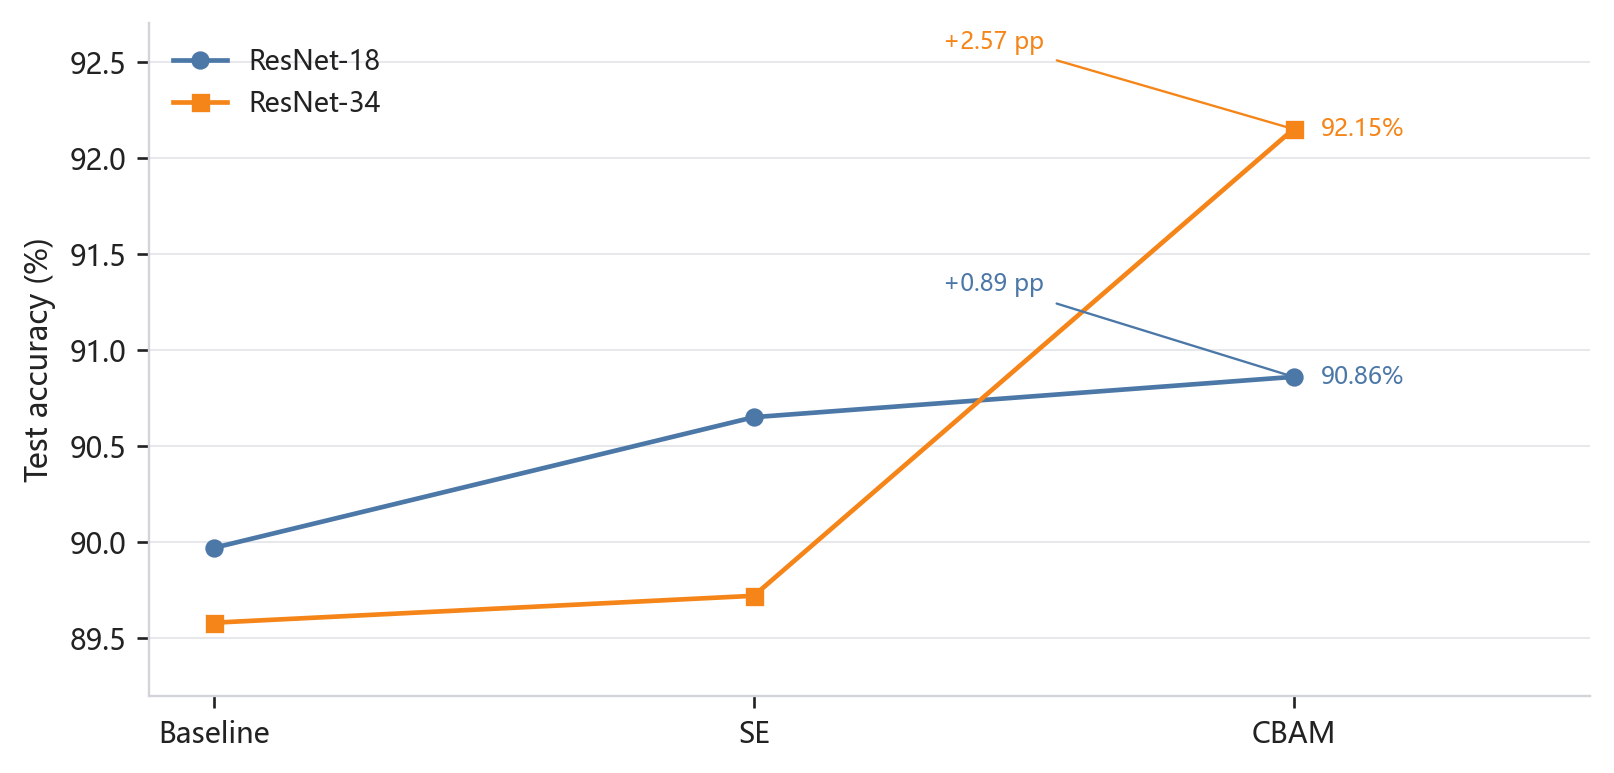
\includegraphics[width=0.72\textwidth]{../tasks/task1_flower_classification/experiment_results/final_report/figures/task1_attention_comparison.png}
    \caption{SE 与 CBAM 注意力模块的测试准确率对比}
    \label{fig:classification-attention-comparison}
\end{figure}

从结果看，CBAM 通常比 SE 更稳定。原因可能在于花卉分类不仅依赖通道语义，还依赖局部区域，例如花心、花瓣边缘和颜色纹理。CBAM 的空间注意力能够进一步强化这些判别区域，因此在 ResNet-18 和 ResNet-34 上均取得更好的测试表现。

\subsection{Transformer 与 ConvNeXt 分析}

Transformer 组整体优于基础 CNN 组。ViT-B/16 的最优测试准确率为 92.83\%，Swin-T 的最优测试准确率为 94.26\%。Swin-T 的优势主要来自两点：首先，shifted window attention 在局部窗口中建模，保留了类似 CNN 的局部归纳偏置，更适合花瓣纹理、边缘与局部形状；其次，窗口移动机制又允许跨区域信息交换，使模型能够同时利用局部细节和全局花型结构。

在扩展 CNN 实验中，ConvNeXt-Tiny 进一步超过了 Swin-T。ConvNeXt-Tiny 同样保留卷积网络的局部归纳偏置，但吸收了现代视觉模型的训练和结构设计。对于 Oxford 102 这样训练集很小、但测试集较大的细粒度分类问题，ConvNeXt-Tiny 的稳定性优于单次 Swin-T 最优结果。

\subsection{超参数影响分析}

从完整网格搜索和补充实验可以观察到以下规律：

\begin{enumerate}
    \item 学习率：对预训练 CNN 来说，\(3\times10^{-4}\) 在 224px 网格中通常比 \(1\times10^{-3}\) 更稳定；Transformer 中 \(1\times10^{-4}\) 的结果明显优于 \(3\times10^{-4}\)，说明预训练 Transformer 微调时更需要较小学习率。最终 ConvNeXt 384px 配置中，\(1\times10^{-4}\) 也优于 \(3\times10^{-4}\) 的候选配置。
    \item Batch size：CNN 中 batch size 32 和 64 都能取得较好结果；Transformer 中最优 Swin-T 使用 batch size 16。最终 ConvNeXt 384px 由于分辨率更高，采用 batch size 16。
    \item Label smoothing：多数最优模型使用 label smoothing=0.1。该策略在小样本细粒度分类中能够缓解过度自信，提升验证集稳定性。
    \item Weight decay：基础 CNN 网格中 \(1\times10^{-4}\) 的最优结果更多；最终 ConvNeXt 384px 配置使用 \(1\times10^{-5}\)，说明更强 backbone 与更高分辨率下可适当减弱权重衰减。
    \item 训练轮数：预训练模型通常在几十个 epoch 内达到最佳验证性能；从零训练模型需要 90--100 个 epoch 以上才达到最佳点，但最终泛化性能仍明显较低。
\end{enumerate}

图 \ref{fig:classification-hyperparameter-heatmap} 进一步把基础预训练 CNN 网格中的学习率和 batch size 关系可视化。每个格子保留同一组学习率与 batch size 下表现最好的 ResNet baseline、SE 或 CBAM 变体。结果显示，\(3\times10^{-4}\) 整体优于 \(1\times10^{-3}\)，而 batch size 64 在该网格中取得最高验证准确率。

\begin{figure}[H]
    \centering
    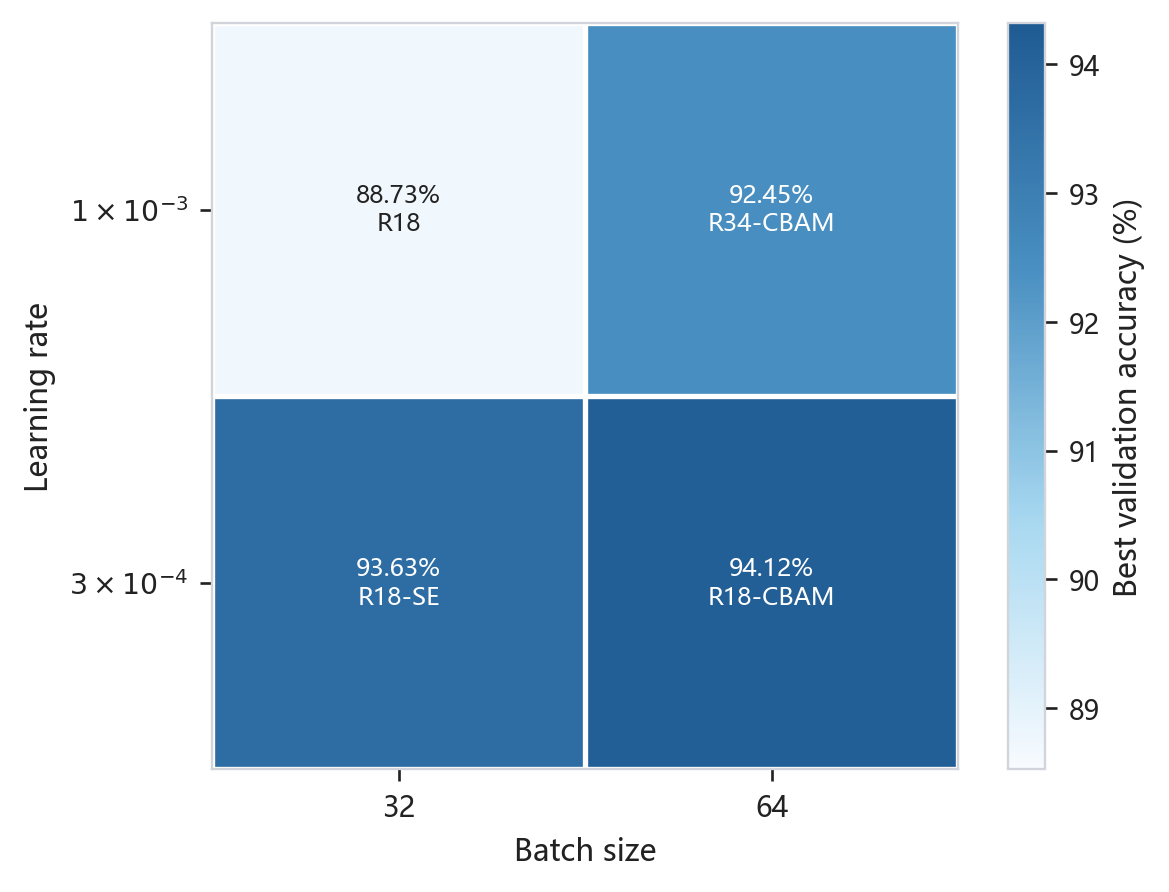
\includegraphics[width=0.58\textwidth]{../tasks/task1_flower_classification/experiment_results/final_report/figures/task1_hyperparameter_heatmap.png}
    \caption{预训练 CNN 网格中学习率与 batch size 的影响}
    \label{fig:classification-hyperparameter-heatmap}
\end{figure}

\subsection{稳定性实验}

最终报告采用 10 个随机种子的平均值作为主结果，而不是挑选单个最高随机种子。虽然其中一个随机种子的单次测试准确率达到 96.50\%，但该值可能带有随机性；10 个随机种子的平均值 \accpm{95.60}{0.61} 更适合作为正式结论。

\begin{table}[H]
    \centering
    \caption{最终 ConvNeXt-Tiny 384px 配置的 10 个随机种子结果}
    \small
    \resizebox{\textwidth}{!}{%
    \begin{tabular}{rrrrr}
        \toprule
        Seed & Best epoch & Epochs completed & Val Acc. & Test Acc. \\
        \midrule
        7 & 30 & 45 & 97.06\% & 95.14\% \\
        42 & 39 & 54 & 97.84\% & 95.85\% \\
        99 & 32 & 47 & 97.55\% & 95.97\% \\
        123 & 51 & 66 & 97.75\% & 96.05\% \\
        314 & 31 & 46 & 97.75\% & 96.50\% \\
        512 & 13 & 28 & 96.67\% & 94.24\% \\
        1009 & 26 & 41 & 96.86\% & 95.54\% \\
        2024 & 34 & 49 & 96.76\% & 95.59\% \\
        2026 & 31 & 46 & 97.75\% & 95.46\% \\
        4096 & 35 & 50 & 96.86\% & 95.67\% \\
        \midrule
        平均 $\pm$ 标准差 & -- & -- & \accpm{97.28}{0.48} & \accpm{95.60}{0.61} \\
        \bottomrule
    \end{tabular}%
    }
\end{table}

\subsection{测试集错误分析}

为了进一步分析最终分类器的错误模式，本文选取最终实验组中测试准确率最高的 seed 314 checkpoint，在官方测试集上重新进行一次逐样本推理。该 checkpoint 对应 ConvNeXt-Tiny 384px 模型，单模型测试准确率为 96.50\%，共正确分类 5934 张，错分 215 张。需要说明的是，报告主结论仍采用 10 个随机种子的平均值；这里使用 seed 314 的目的是观察一个代表性最优单模型在测试集上的具体错误分布。

由于 Oxford 102 的官方标注文件只提供类别编号，下面的错误分析沿用数据集中的 1--102 类编号。表 \ref{tab:classification-top-confusions} 和图 \ref{fig:classification-top-confusions} 展示了出现次数最多的类别混淆。最明显的错误是第 96 类被预测为第 97 类，共 10 张，占第 96 类测试样本的 14.08\%；第 53 类被预测为第 46 类也出现了 9 次。其余混淆对的绝对次数明显更低，说明模型并不是在大范围类别上系统性失效，而是在若干细粒度边界上仍存在不确定性。

\begin{table}[H]
    \centering
    \caption{最终 ConvNeXt-Tiny 384px 模型的主要错分类别对}
    \label{tab:classification-top-confusions}
    \small
    \begin{tabular}{rrrrr}
        \toprule
        排名 & 真实类别 & 预测类别 & 错分数量 & 占真实类比例 \\
        \midrule
        1 & 96 & 97 & 10 & 14.08\% \\
        2 & 53 & 46 & 9 & 12.33\% \\
        3 & 51 & 83 & 7 & 2.94\% \\
        4 & 23 & 97 & 5 & 7.04\% \\
        5 & 50 & 12 & 4 & 5.56\% \\
        6 & 51 & 75 & 4 & 1.68\% \\
        7 & 51 & 1 & 4 & 1.68\% \\
        8 & 51 & 19 & 4 & 1.68\% \\
        \bottomrule
    \end{tabular}
\end{table}

\begin{figure}[H]
    \centering
    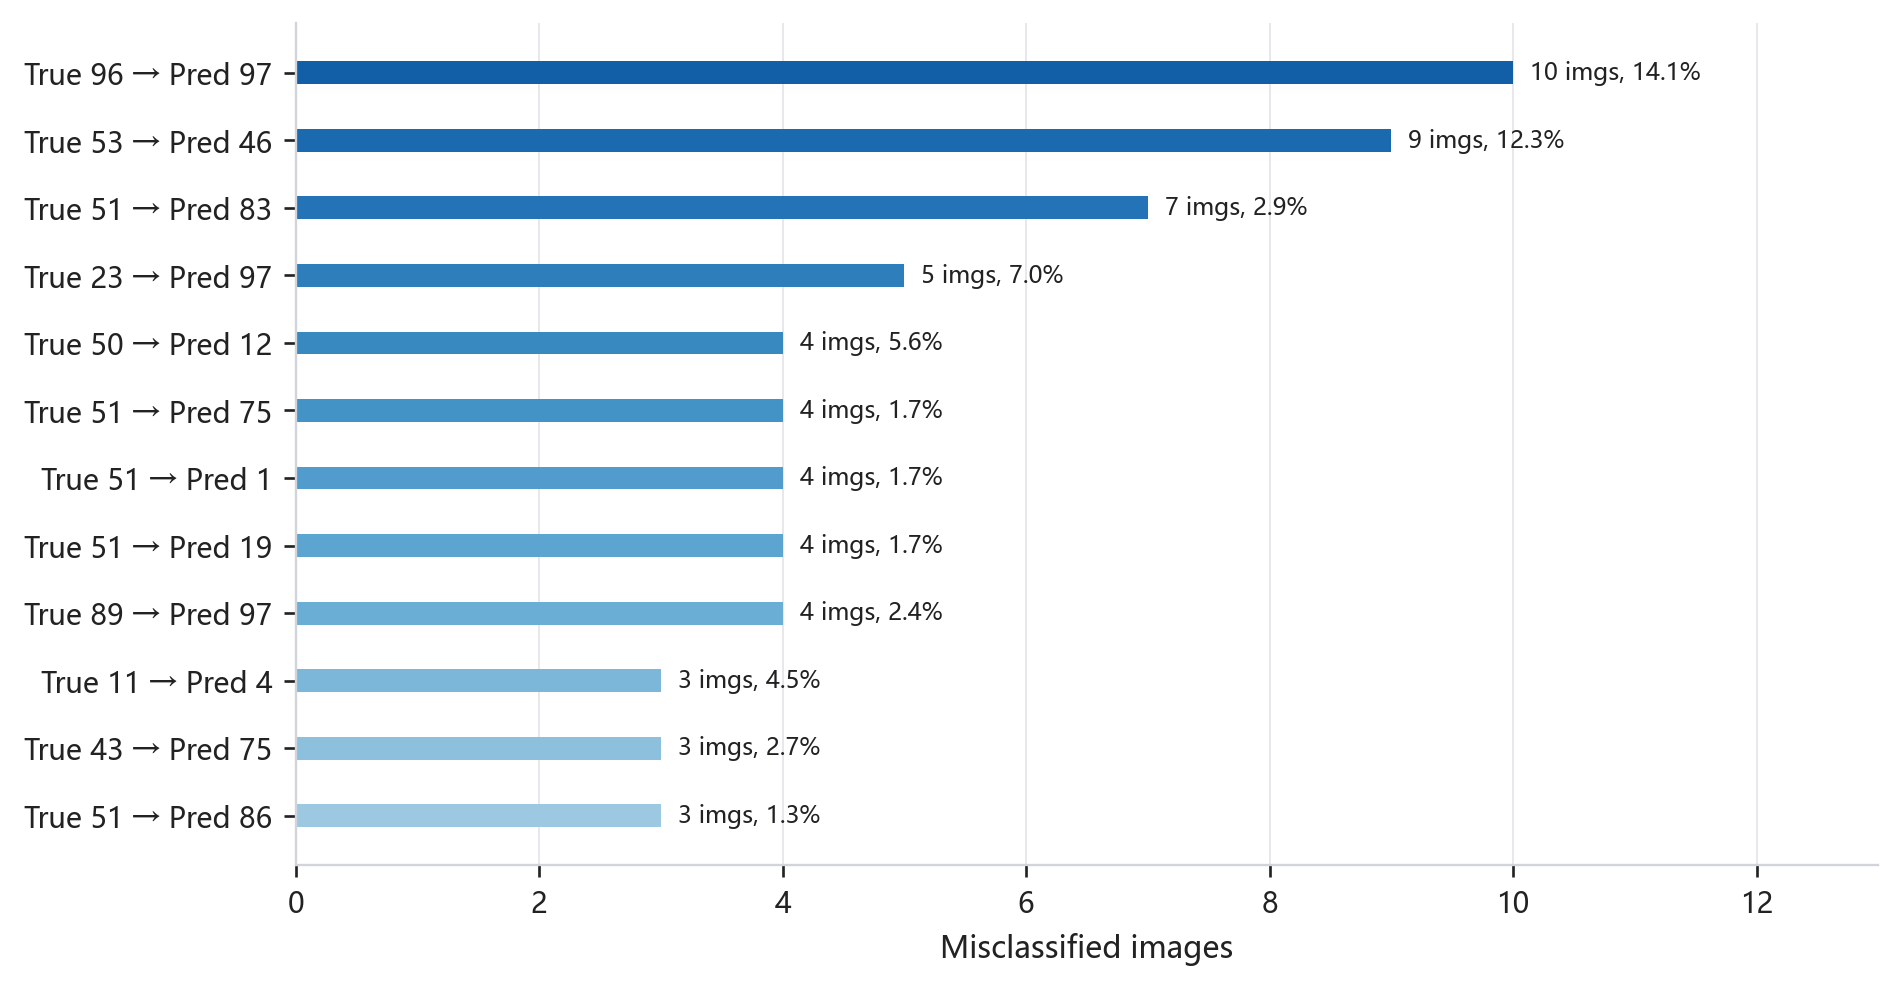
\includegraphics[width=0.78\textwidth]{../tasks/task1_flower_classification/experiment_results/final_report/figures/task1_convnext384_top_confusions.png}
    \caption{最终 ConvNeXt-Tiny 384px 模型的高频错分类别对}
    \label{fig:classification-top-confusions}
\end{figure}

图 \ref{fig:classification-misclassified-examples} 进一步列出了一组高置信度错分样例。可以看到，这些错误通常不是由图像完全失真导致的，而是与花瓣形状、花心结构、颜色组合、拍摄角度和遮挡等细节有关。例如第 96 类多次被预测为第 97 类，样例中花瓣轮廓和颜色分布非常接近；第 50 类与第 12 类的混淆则体现出黄色花卉在局部纹理和花型相似时仍然具有较强挑战性。这说明即使最终模型已经达到较高准确率，Oxford 102 的剩余错误仍主要来自细粒度视觉差异，而不是训练过程没有收敛或模型整体表达能力不足。

\begin{figure}[htbp]
    \centering
    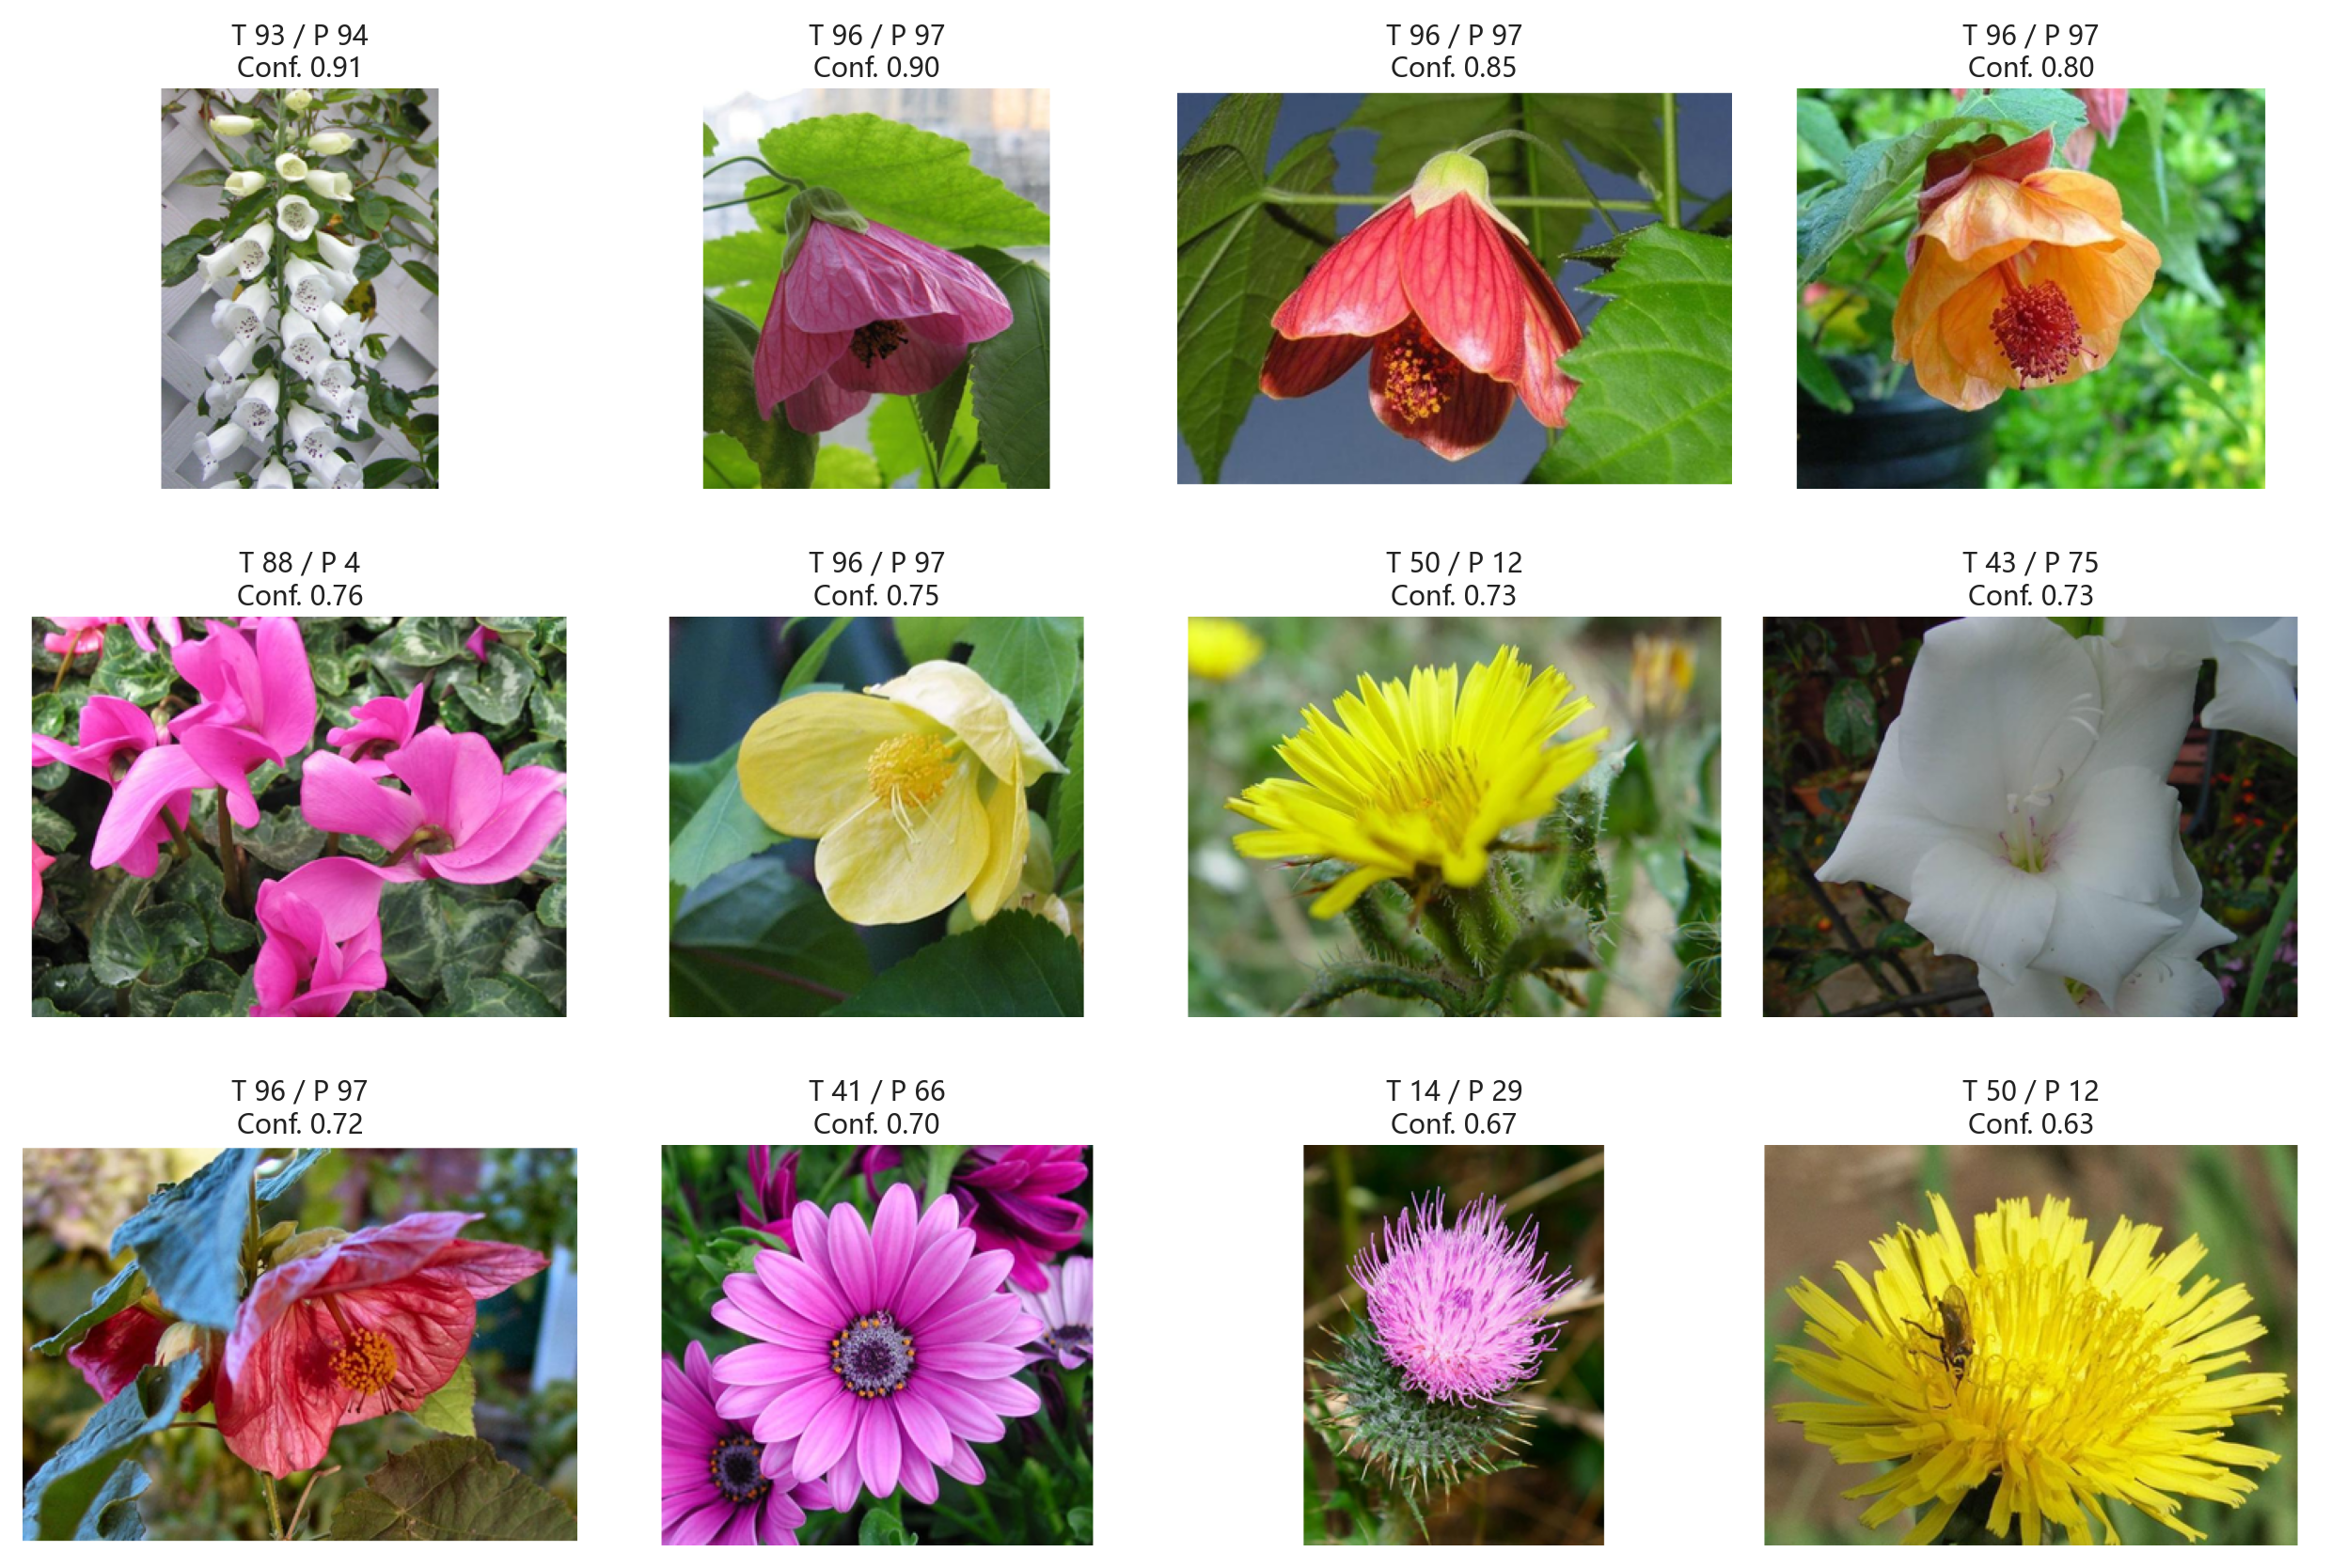
\includegraphics[width=0.88\textwidth]{../tasks/task1_flower_classification/experiment_results/final_report/figures/task1_convnext384_misclassified_examples.png}
    \caption{最终 ConvNeXt-Tiny 384px 模型的高置信度错分样例；T 表示真实类别，P 表示预测类别}
    \label{fig:classification-misclassified-examples}
\end{figure}

\section{道路车辆检测与跟踪实验}

\subsection{数据集与模型设置}

道路车辆检测实验使用 Road Vehicle Images Dataset。数据以 YOLO 检测格式组织，每个标注框由类别编号和归一化后的中心点、宽高表示。训练集包含 2704 张图像和 21764 个标注实例，验证集包含 300 张图像和 2584 个标注实例。数据集类别数为 21，覆盖 ambulance、bus、car、motorbike、rickshaw、suv、truck、van 等道路场景中常见交通参与者。相较于单一车辆类别检测，该数据集的难点在于类别之间外观相近、目标尺度差异较大，并且部分类别样本较少。

实验使用 YOLOv8s 作为检测器，并基于 \code{yolov8s.pt} 预训练权重微调。YOLO 系列模型将目标定位和类别预测放在同一个端到端网络中完成，适合道路视频中的实时检测。YOLOv8s 在模型规模和检测精度之间较为平衡，能够在有限计算资源下完成多类别车辆检测实验。训练时使用 AdamW 优化器，输入分辨率为 640，batch size 为 16，并保留 YOLO 默认的数据增强策略，包括 HSV 颜色扰动、随机平移、尺度缩放、水平翻转和 mosaic 增强。这些增强有助于提高模型对不同拍摄角度、光照条件和目标尺度的鲁棒性。

\begin{table}[H]
    \centering
    \caption{道路车辆检测数据集概况}
    \small
    \begin{tabular}{lr}
        \toprule
        项目 & 数值 \\
        \midrule
        训练图像数 & 2704 \\
        验证图像数 & 300 \\
        训练集标注实例数 & 21764 \\
        验证集标注实例数 & 2584 \\
        平均每图实例数 & 8.11 \\
        检测类别数 & 21 \\
        输入标注格式 & YOLO bounding box \\
        \bottomrule
    \end{tabular}
\end{table}

图 \ref{fig:detection-dataset-samples} 给出了道路车辆数据中的标注样例。可以看到，同一图像中往往同时出现多辆车、行人相关交通工具以及远处小目标，标注框尺度差异明显；部分目标还会被车体、道路设施或画面边缘遮挡。这些因素使检测器不仅需要区分类别，还需要在密集场景中保持较好的框定位精度。

\begin{figure}[htbp]
    \centering
    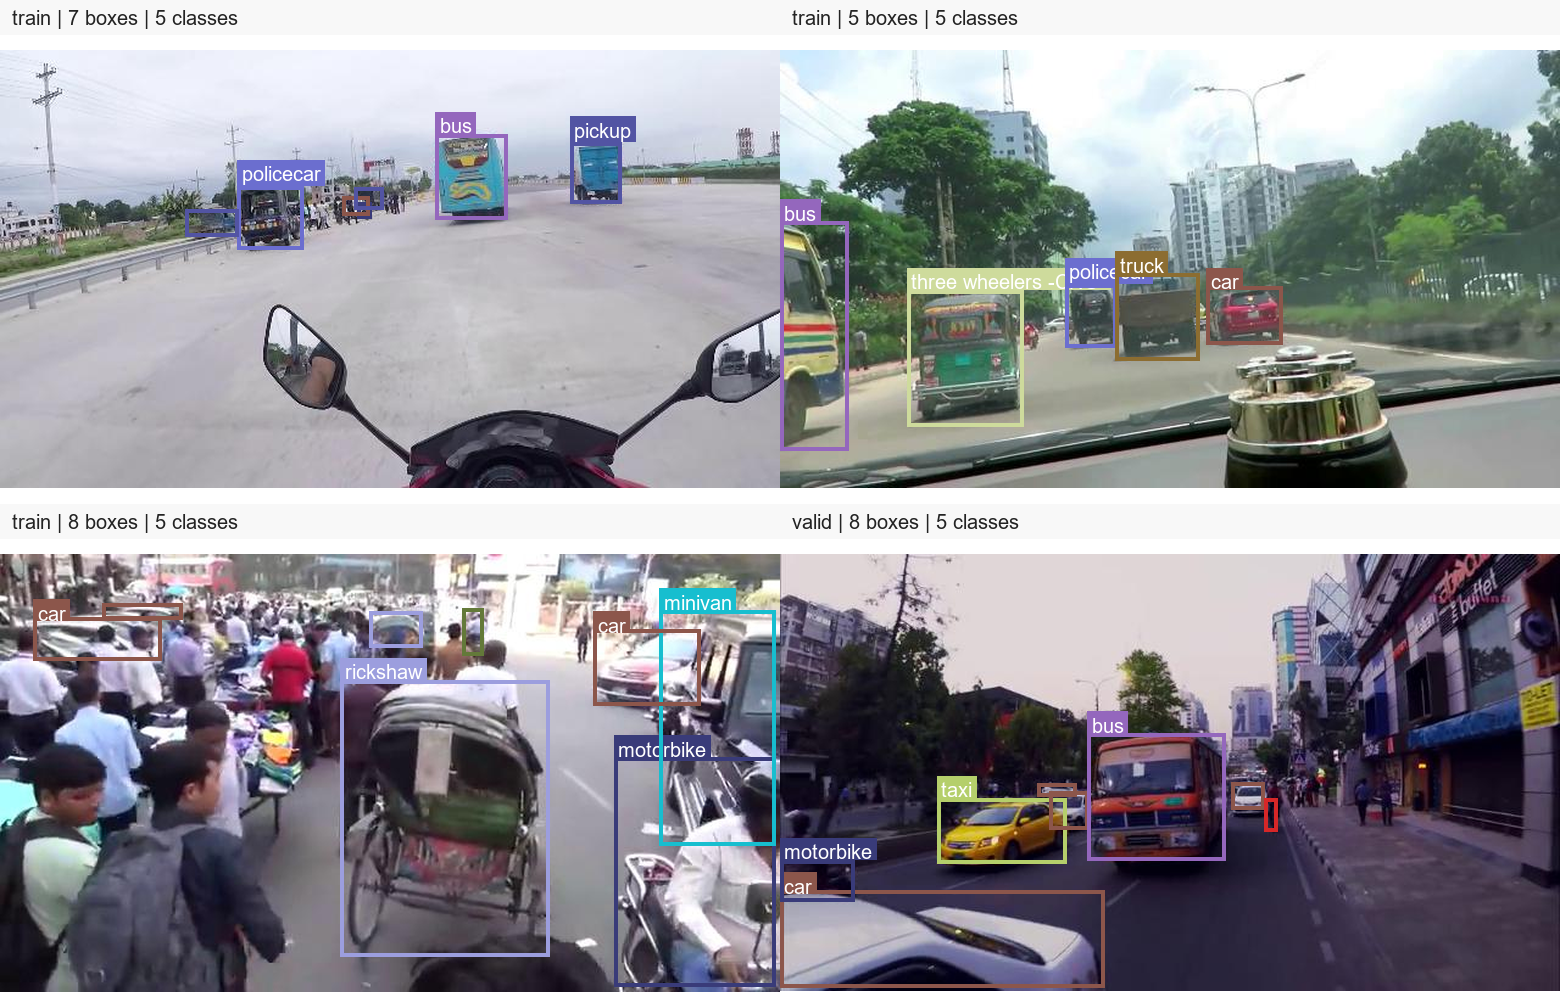
\includegraphics[width=0.92\textwidth]{../tasks/task2_road_vehicle_detection/report_figures/detection_dataset_samples.png}
    \caption{Road Vehicle Images Dataset 标注样例}
    \label{fig:detection-dataset-samples}
\end{figure}

进一步统计训练集和验证集的全部 YOLO 标注，类别实例分布如图 \ref{fig:detection-class-distribution} 所示，横轴使用对数尺度。car、rickshaw、bus、three wheelers-CNG 和 motorbike 是最主要的五类，共占据大部分训练信号；而 garbagevan、policecar、scooter、army vehicle、taxi 等类别样本很少。类别长尾分布会使模型更偏向高频类别，同时也解释了后续部分类别虽然整体检测器可用、但类别级 mAP 差异较大的现象。对于 van、suv、pickup、minivan 等外观相近类别，样本数量并不是唯一瓶颈，车辆轮廓和拍摄角度的相似性同样会增加混淆。

\begin{figure}[htbp]
    \centering
    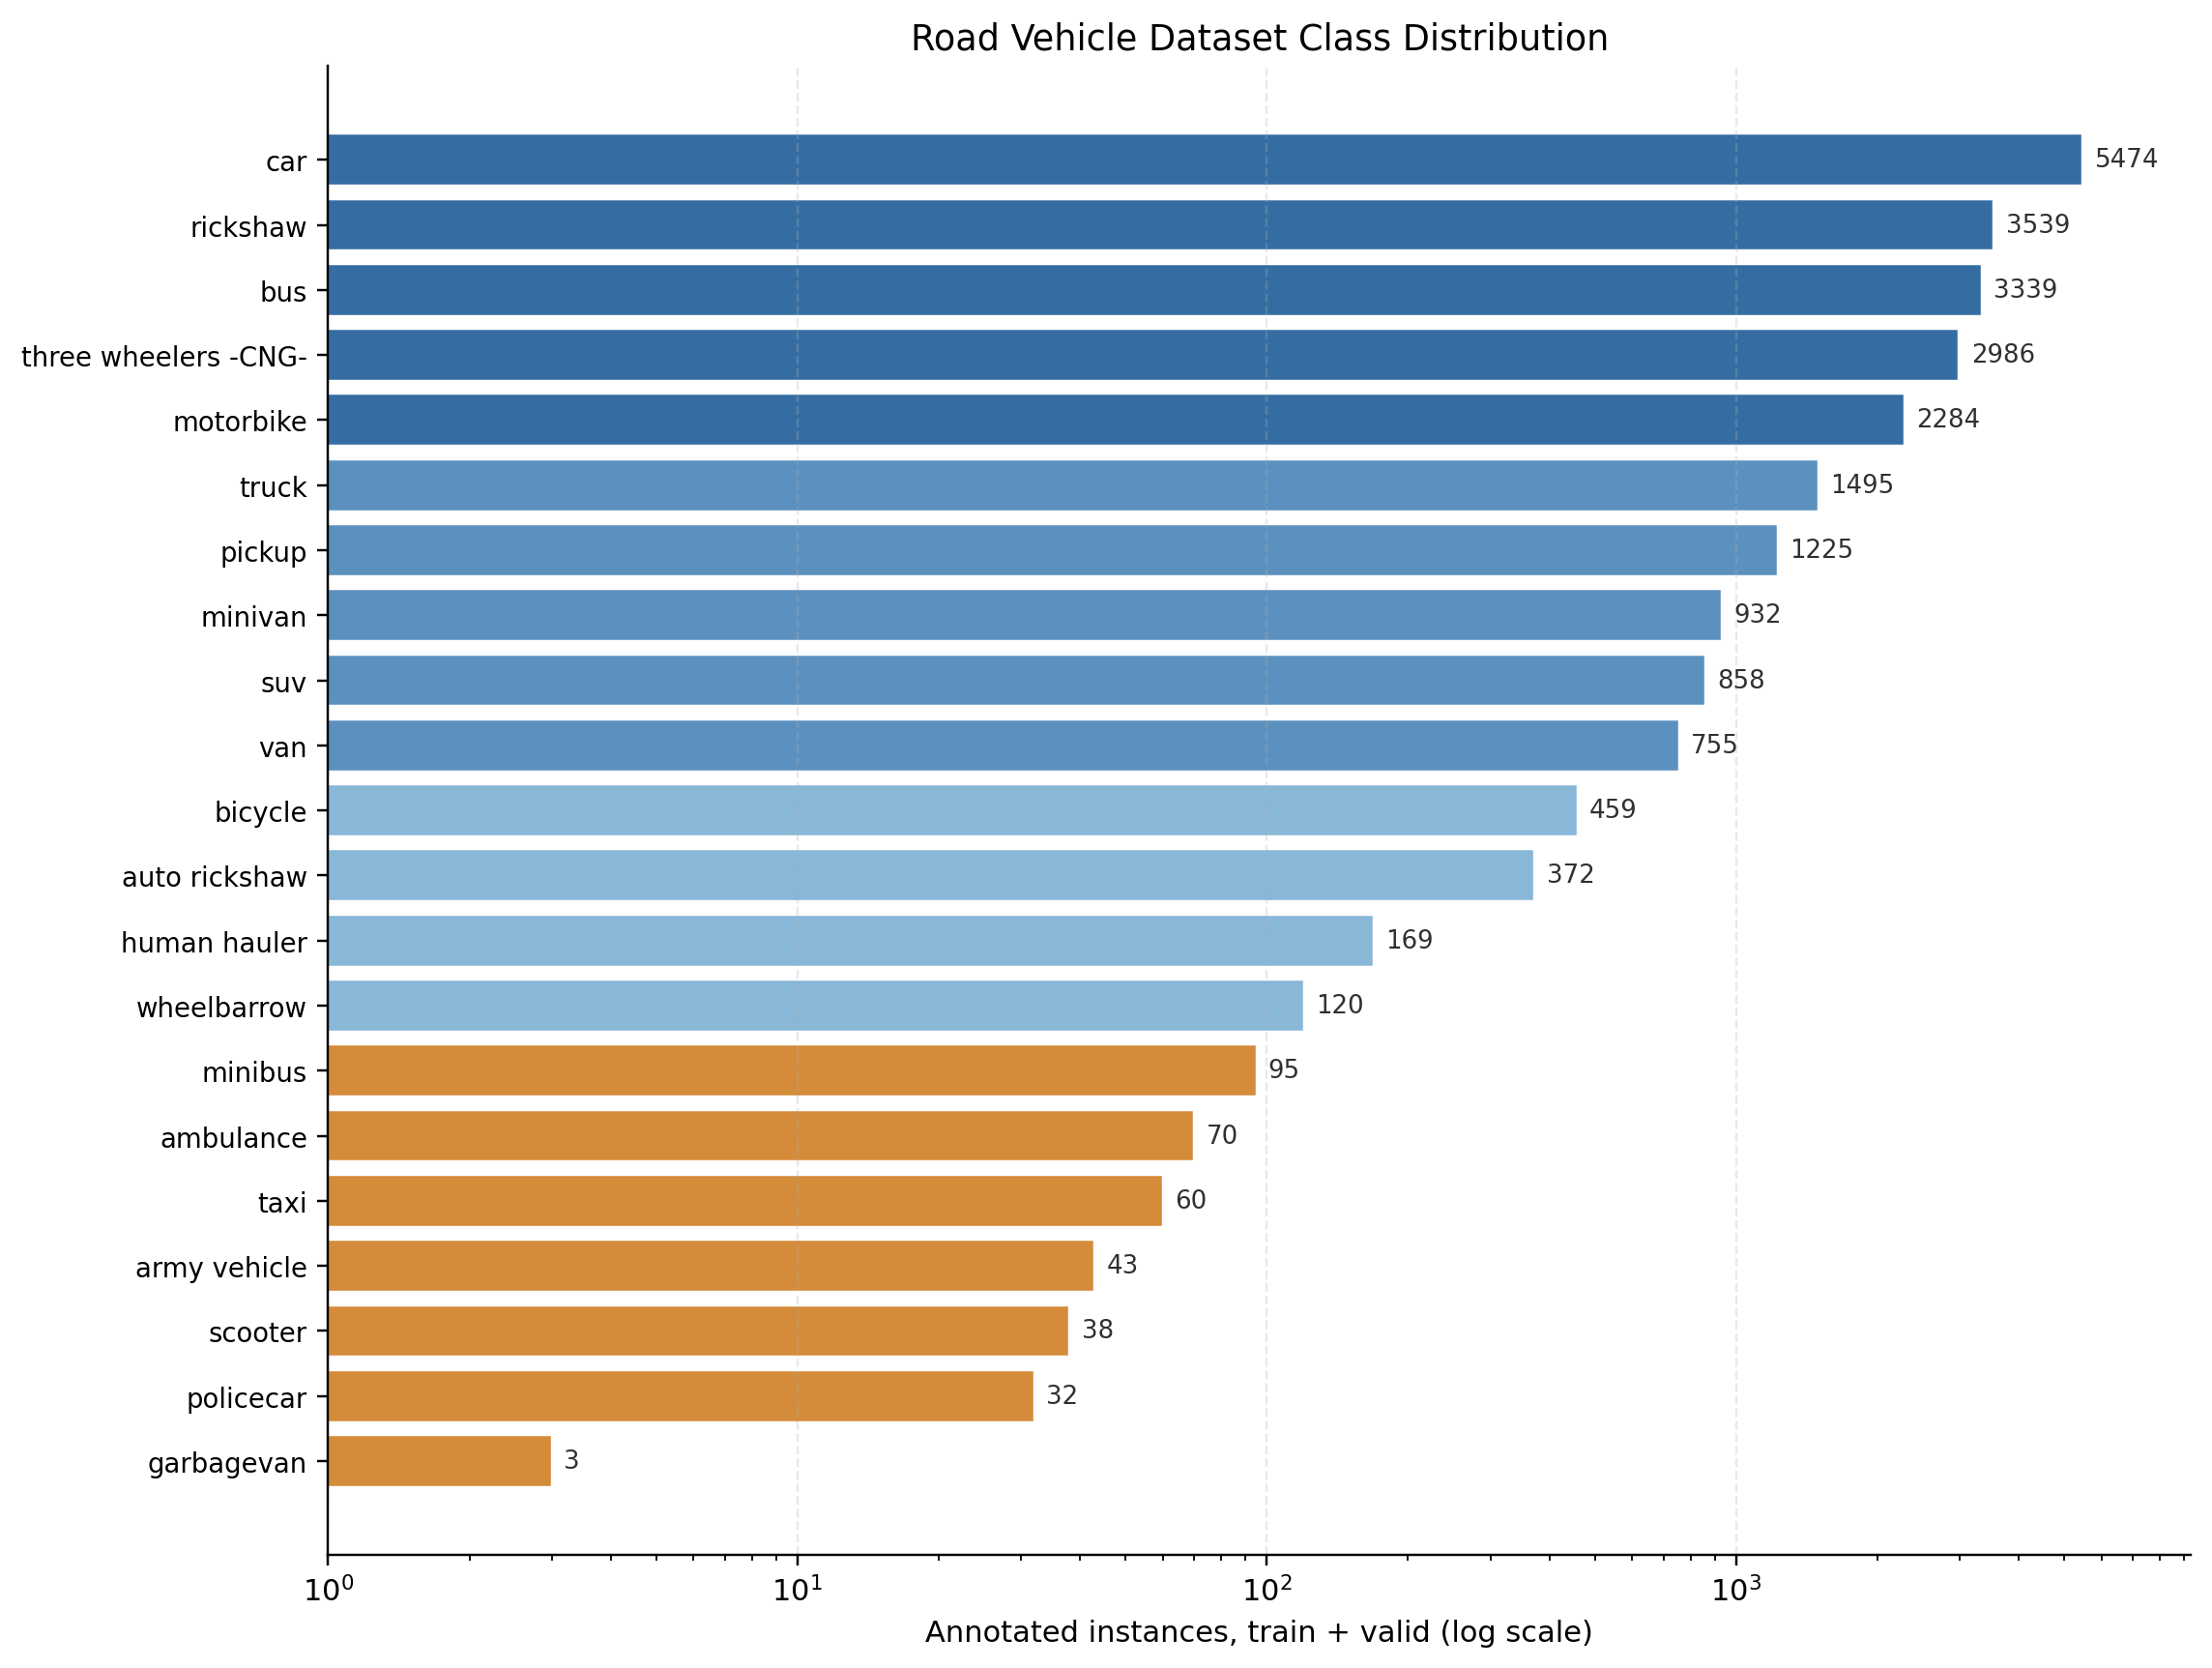
\includegraphics[width=0.80\textwidth]{../tasks/task2_road_vehicle_detection/report_figures/detection_class_distribution.png}
    \caption{道路车辆检测类别实例分布}
    \label{fig:detection-class-distribution}
\end{figure}

\begin{table}[H]
    \centering
    \caption{YOLOv8s 训练配置}
    \small
    \begin{tabular}{ll}
        \toprule
        Setting & Value \\
        \midrule
        Model & YOLOv8s \\
        Pretrained weights & \code{yolov8s.pt} \\
        Dataset classes & 21 \\
        Image size & 640 \\
        Batch size & 16 \\
        Optimizer & AdamW \\
        Initial learning rate & 0.001 \\
        Max epochs & 100 \\
        Early stopping patience & 10 \\
        Actual epochs & 37 \\
        Best epoch & 27 \\
        \bottomrule
    \end{tabular}
\end{table}

训练与验证过程同时保存了 Ultralytics 本地可视化文件，并同步到 Weights \& Biases。W\&B 项目为 \href{https://wandb.ai/crepuscule-fudan/HW2_Road_Vehicle_Detection}{HW2\_Road\_Vehicle\_Detection}，对应运行为 \href{https://wandb.ai/crepuscule-fudan/HW2_Road_Vehicle_Detection/runs/v7f1dr6d}{v7f1dr6d / yolov8s\_adamw\_lr001\_v2}。报告中的训练曲线、PR/F1 曲线和混淆矩阵主要来自本地 \code{plots=True} 生成的可视化结果，并与 W\&B 记录的训练过程一致。

训练原计划最多运行 100 个 epoch，但验证集指标在第 27 个 epoch 附近达到较优水平，随后提升不再稳定，最终触发 patience 为 10 的 early stopping，并在第 37 个 epoch 停止。训练过程显示，模型的 box loss、classification loss 和 DFL loss 均随 epoch 增加而下降，说明网络逐渐学会了车辆位置回归和类别判别；但验证集 mAP 在后期存在波动，反映出多类别车辆检测中的小目标、遮挡和类别相似性仍会限制泛化表现。

\subsection{检测结果}

验证集指标如表 \ref{tab:detection-metrics} 所示。Precision 为 0.667，Recall 为 0.412，说明检测结果中预测框的准确性较好，但仍有较多真实目标没有被召回。mAP50 为 0.520，说明在 IoU 阈值为 0.5 时，模型对主要车辆类别已经形成了可用的检测能力；mAP50-95 为 0.304，明显低于 mAP50，说明在更严格的定位标准下，框的位置精度和小目标定位仍是主要瓶颈。

\begin{table}[H]
    \centering
    \caption{车辆检测验证集指标}
    \label{tab:detection-metrics}
    \small
    \begin{tabular}{lr}
        \toprule
        Metric & Value \\
        \midrule
        Precision & 0.667 \\
        Recall & 0.412 \\
        mAP50 & 0.520 \\
        mAP50-95 & 0.304 \\
        \bottomrule
    \end{tabular}
\end{table}

从训练曲线可以看到，mAP50 在前 20 多个 epoch 中持续提升，随后进入平台期并出现震荡。第 36 个 epoch 的 recall 曾达到 0.558，但 precision 降至 0.498；而最终最佳权重的 precision 更高、recall 较低，说明模型更倾向于保守预测。这种 precision-recall 权衡在道路车辆检测中比较常见：降低置信度阈值可以召回更多车辆，但也会引入更多误检；提高阈值则可以减少误检，但容易漏掉远处、被遮挡或尺寸较小的车辆。

\begin{table}[H]
    \centering
    \caption{代表性类别 mAP50}
    \small
    \begin{tabular}{lr}
        \toprule
        Class & mAP50 \\
        \midrule
        car & 0.790 \\
        rickshaw & 0.733 \\
        three wheelers -CNG- & 0.724 \\
        bus & 0.663 \\
        truck & 0.624 \\
        van & 0.246 \\
        suv & 0.188 \\
        \bottomrule
    \end{tabular}
\end{table}

类别级结果表明，car、rickshaw、three wheelers-CNG、bus 和 truck 等较常见或外观边界较清晰的类别 mAP50 较高。其中 car 的 mAP50 达到 0.790，是最容易识别的类别之一；rickshaw 和 three wheelers-CNG 的检测效果也相对较好，说明模型能够学习到这类交通工具的形状特征。相比之下，van 和 suv 的 mAP50 分别只有 0.246 和 0.188，说明数据集中其他少样本或外观相似类别更容易互相混淆，例如 minivan、van、suv、pickup 等类别之间的轮廓差异较细，容易受到拍摄角度和遮挡影响。

\begin{figure}[H]
    \centering
    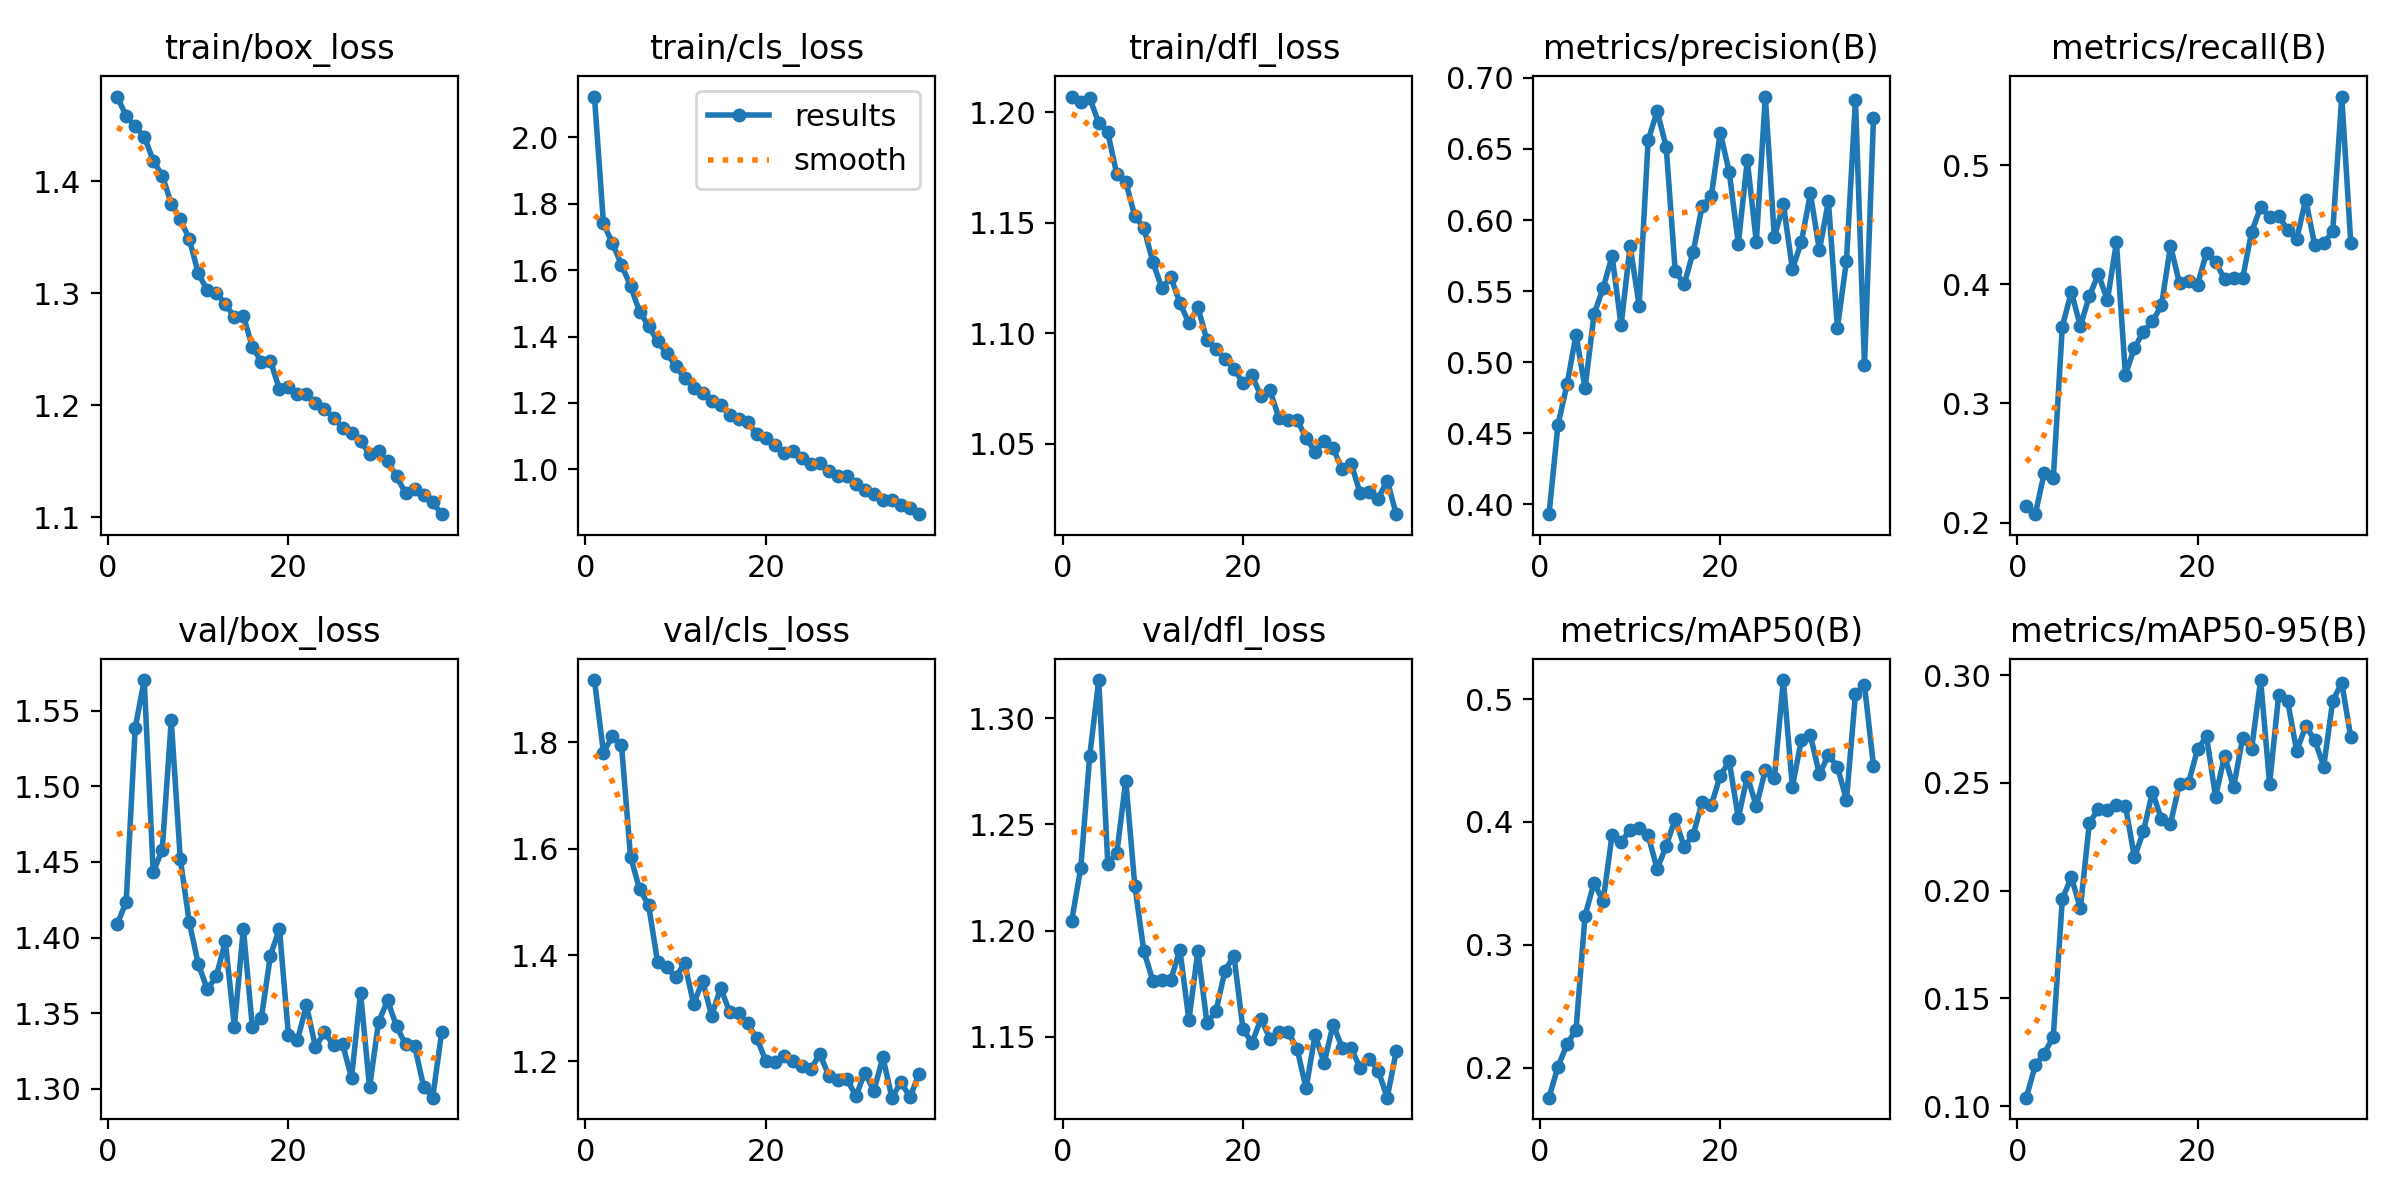
\includegraphics[width=0.95\textwidth]{../tasks/task2_road_vehicle_detection/train_results/results.png}
    \caption{YOLOv8s 训练曲线}
\end{figure}

\begin{figure}[H]
    \centering
    \begin{subfigure}{0.48\textwidth}
        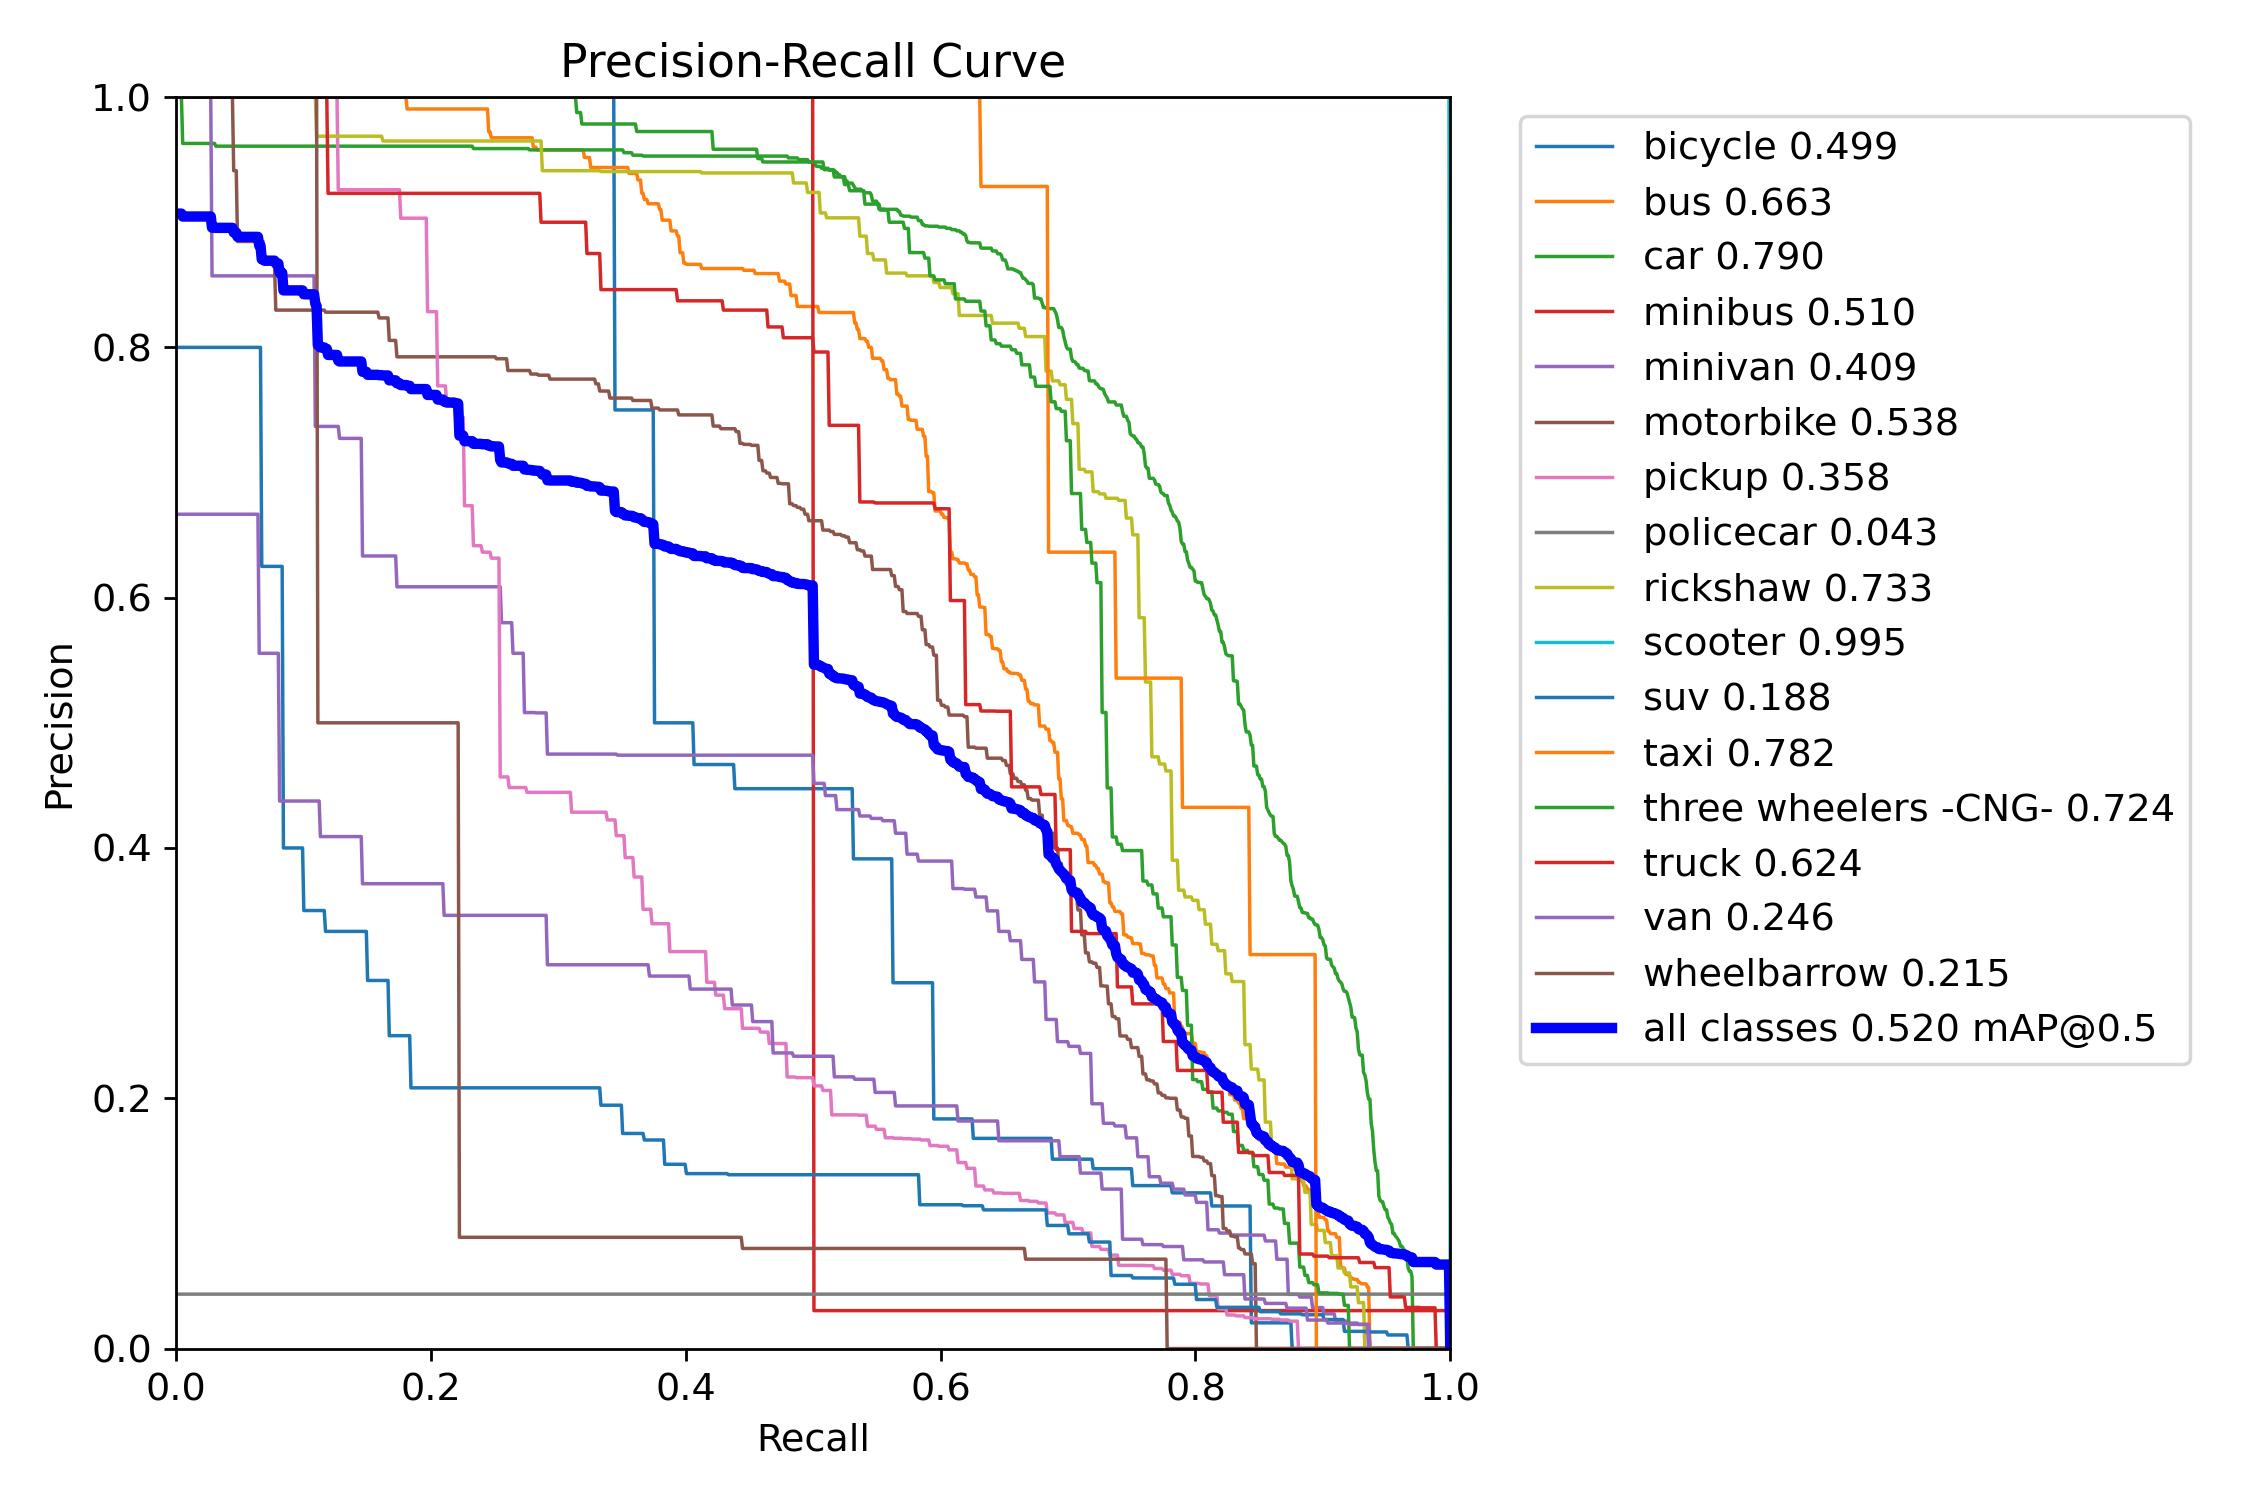
\includegraphics[width=\textwidth]{../tasks/task2_road_vehicle_detection/train_results/BoxPR_curve.png}
        \caption{Precision-recall 曲线}
    \end{subfigure}
    \hfill
    \begin{subfigure}{0.48\textwidth}
        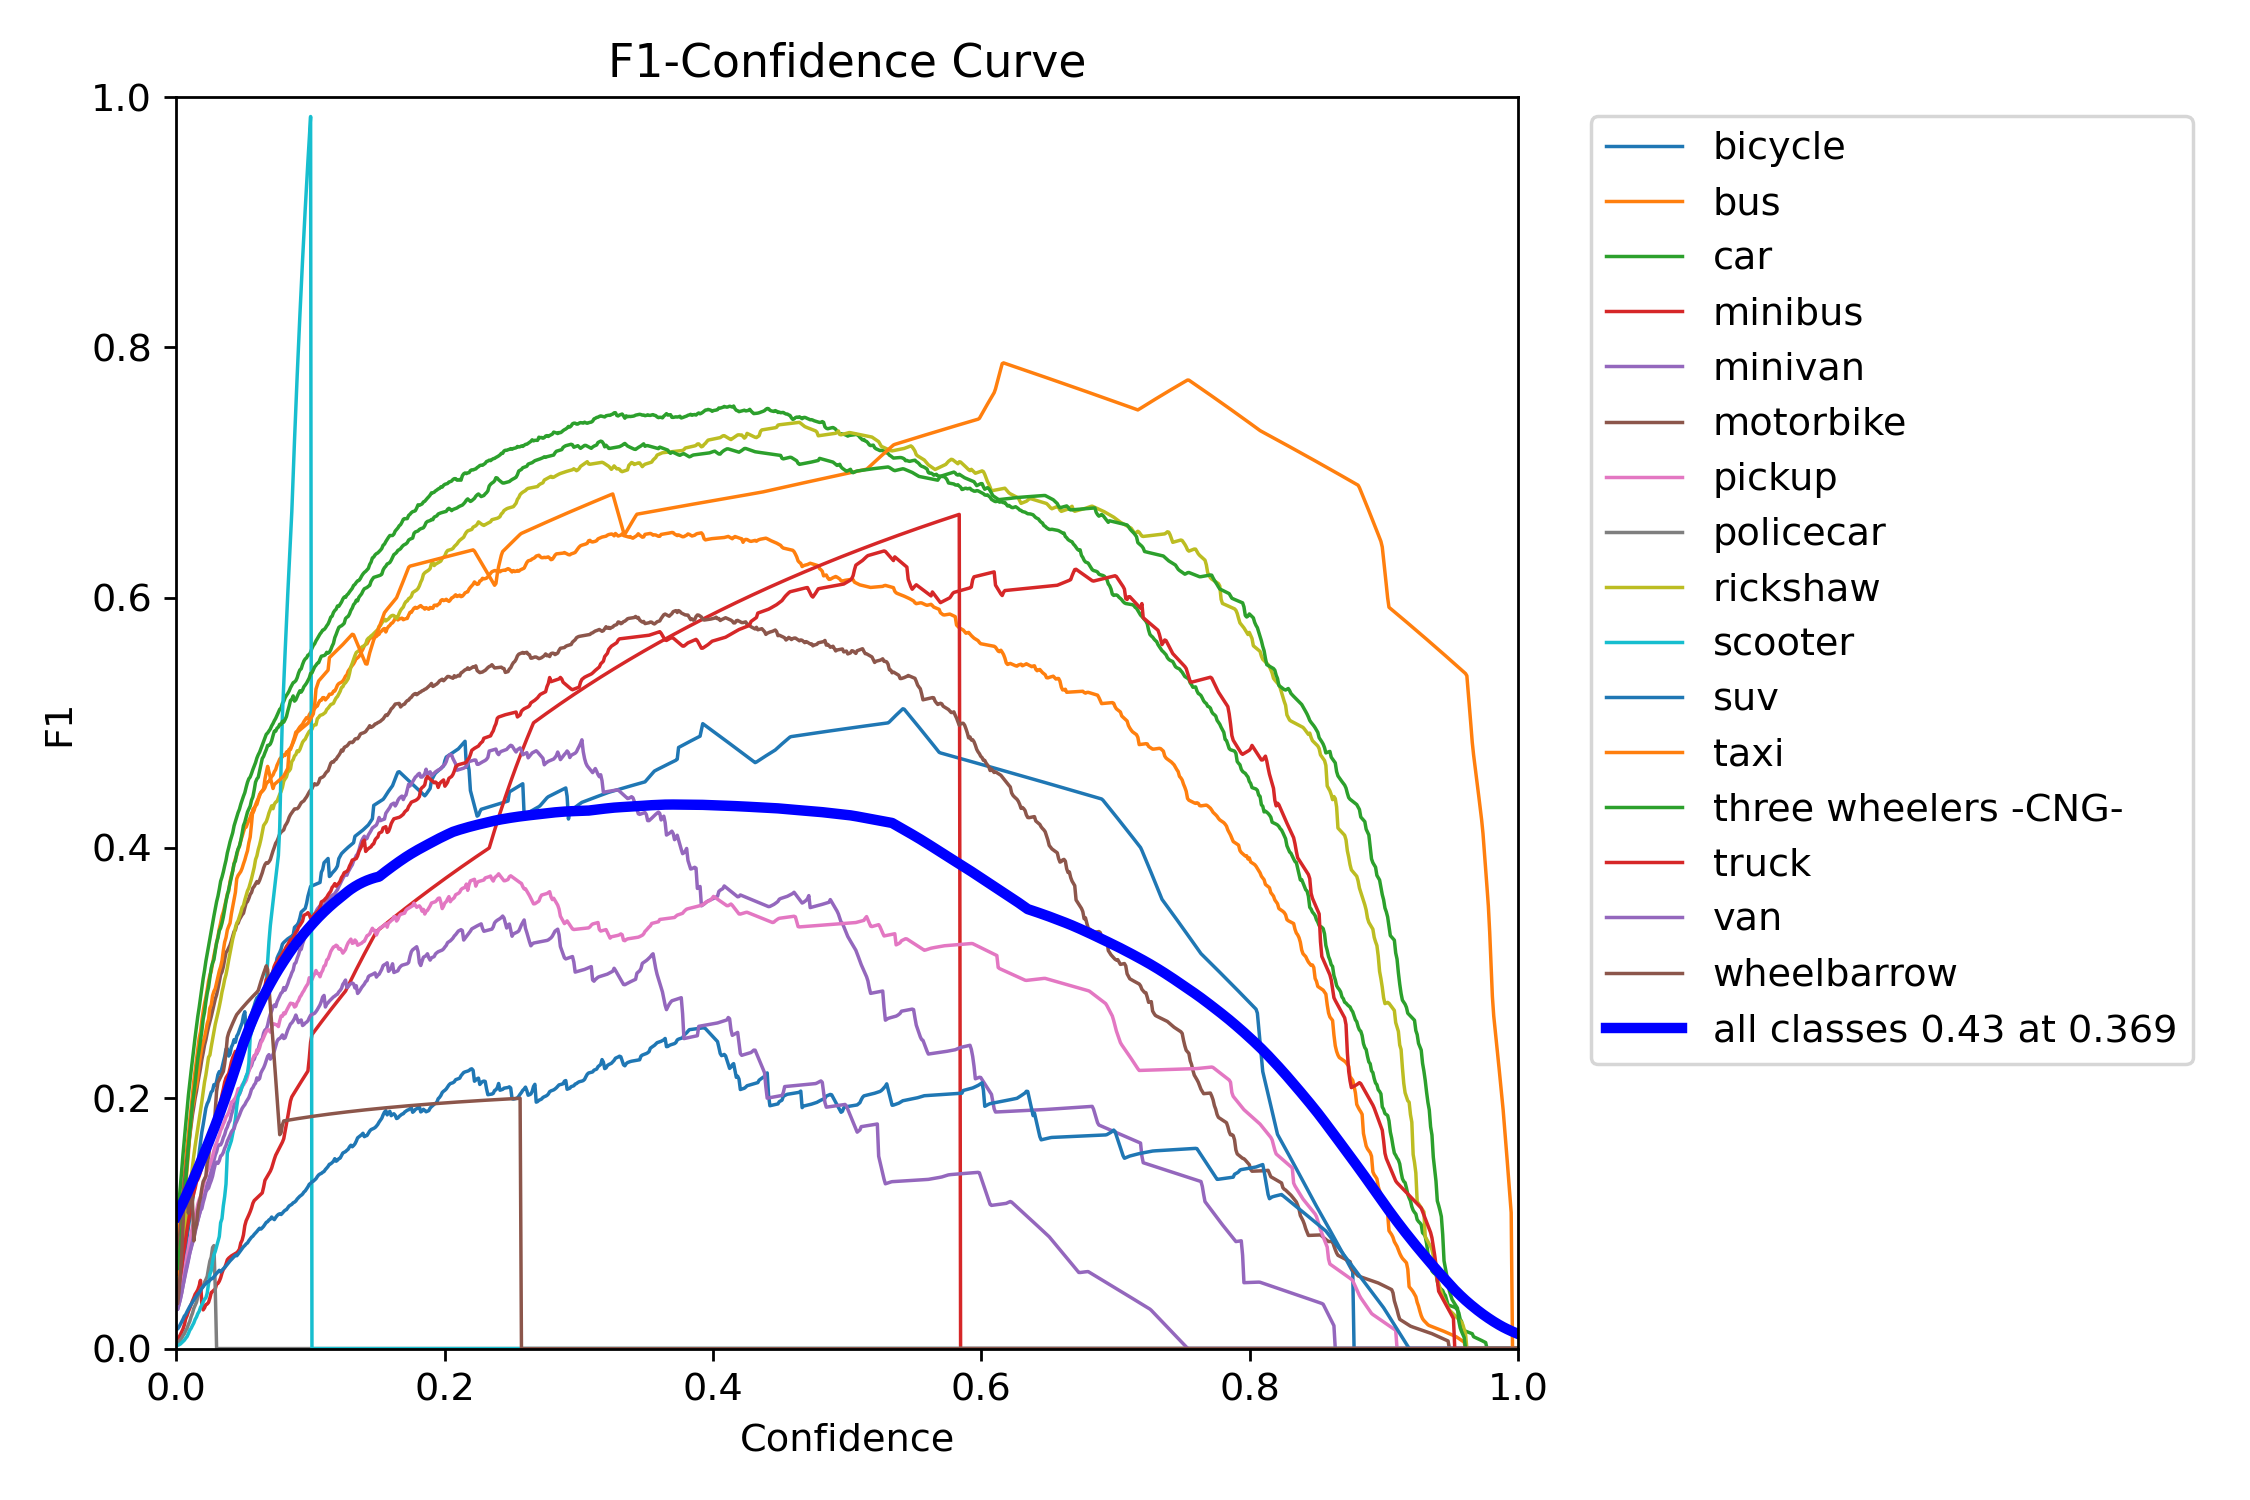
\includegraphics[width=\textwidth]{../tasks/task2_road_vehicle_detection/train_results/BoxF1_curve.png}
        \caption{F1-confidence 曲线}
    \end{subfigure}
    \caption{YOLOv8s 检测阈值相关曲线}
\end{figure}

\begin{figure}[H]
    \centering
    \begin{subfigure}{0.48\textwidth}
        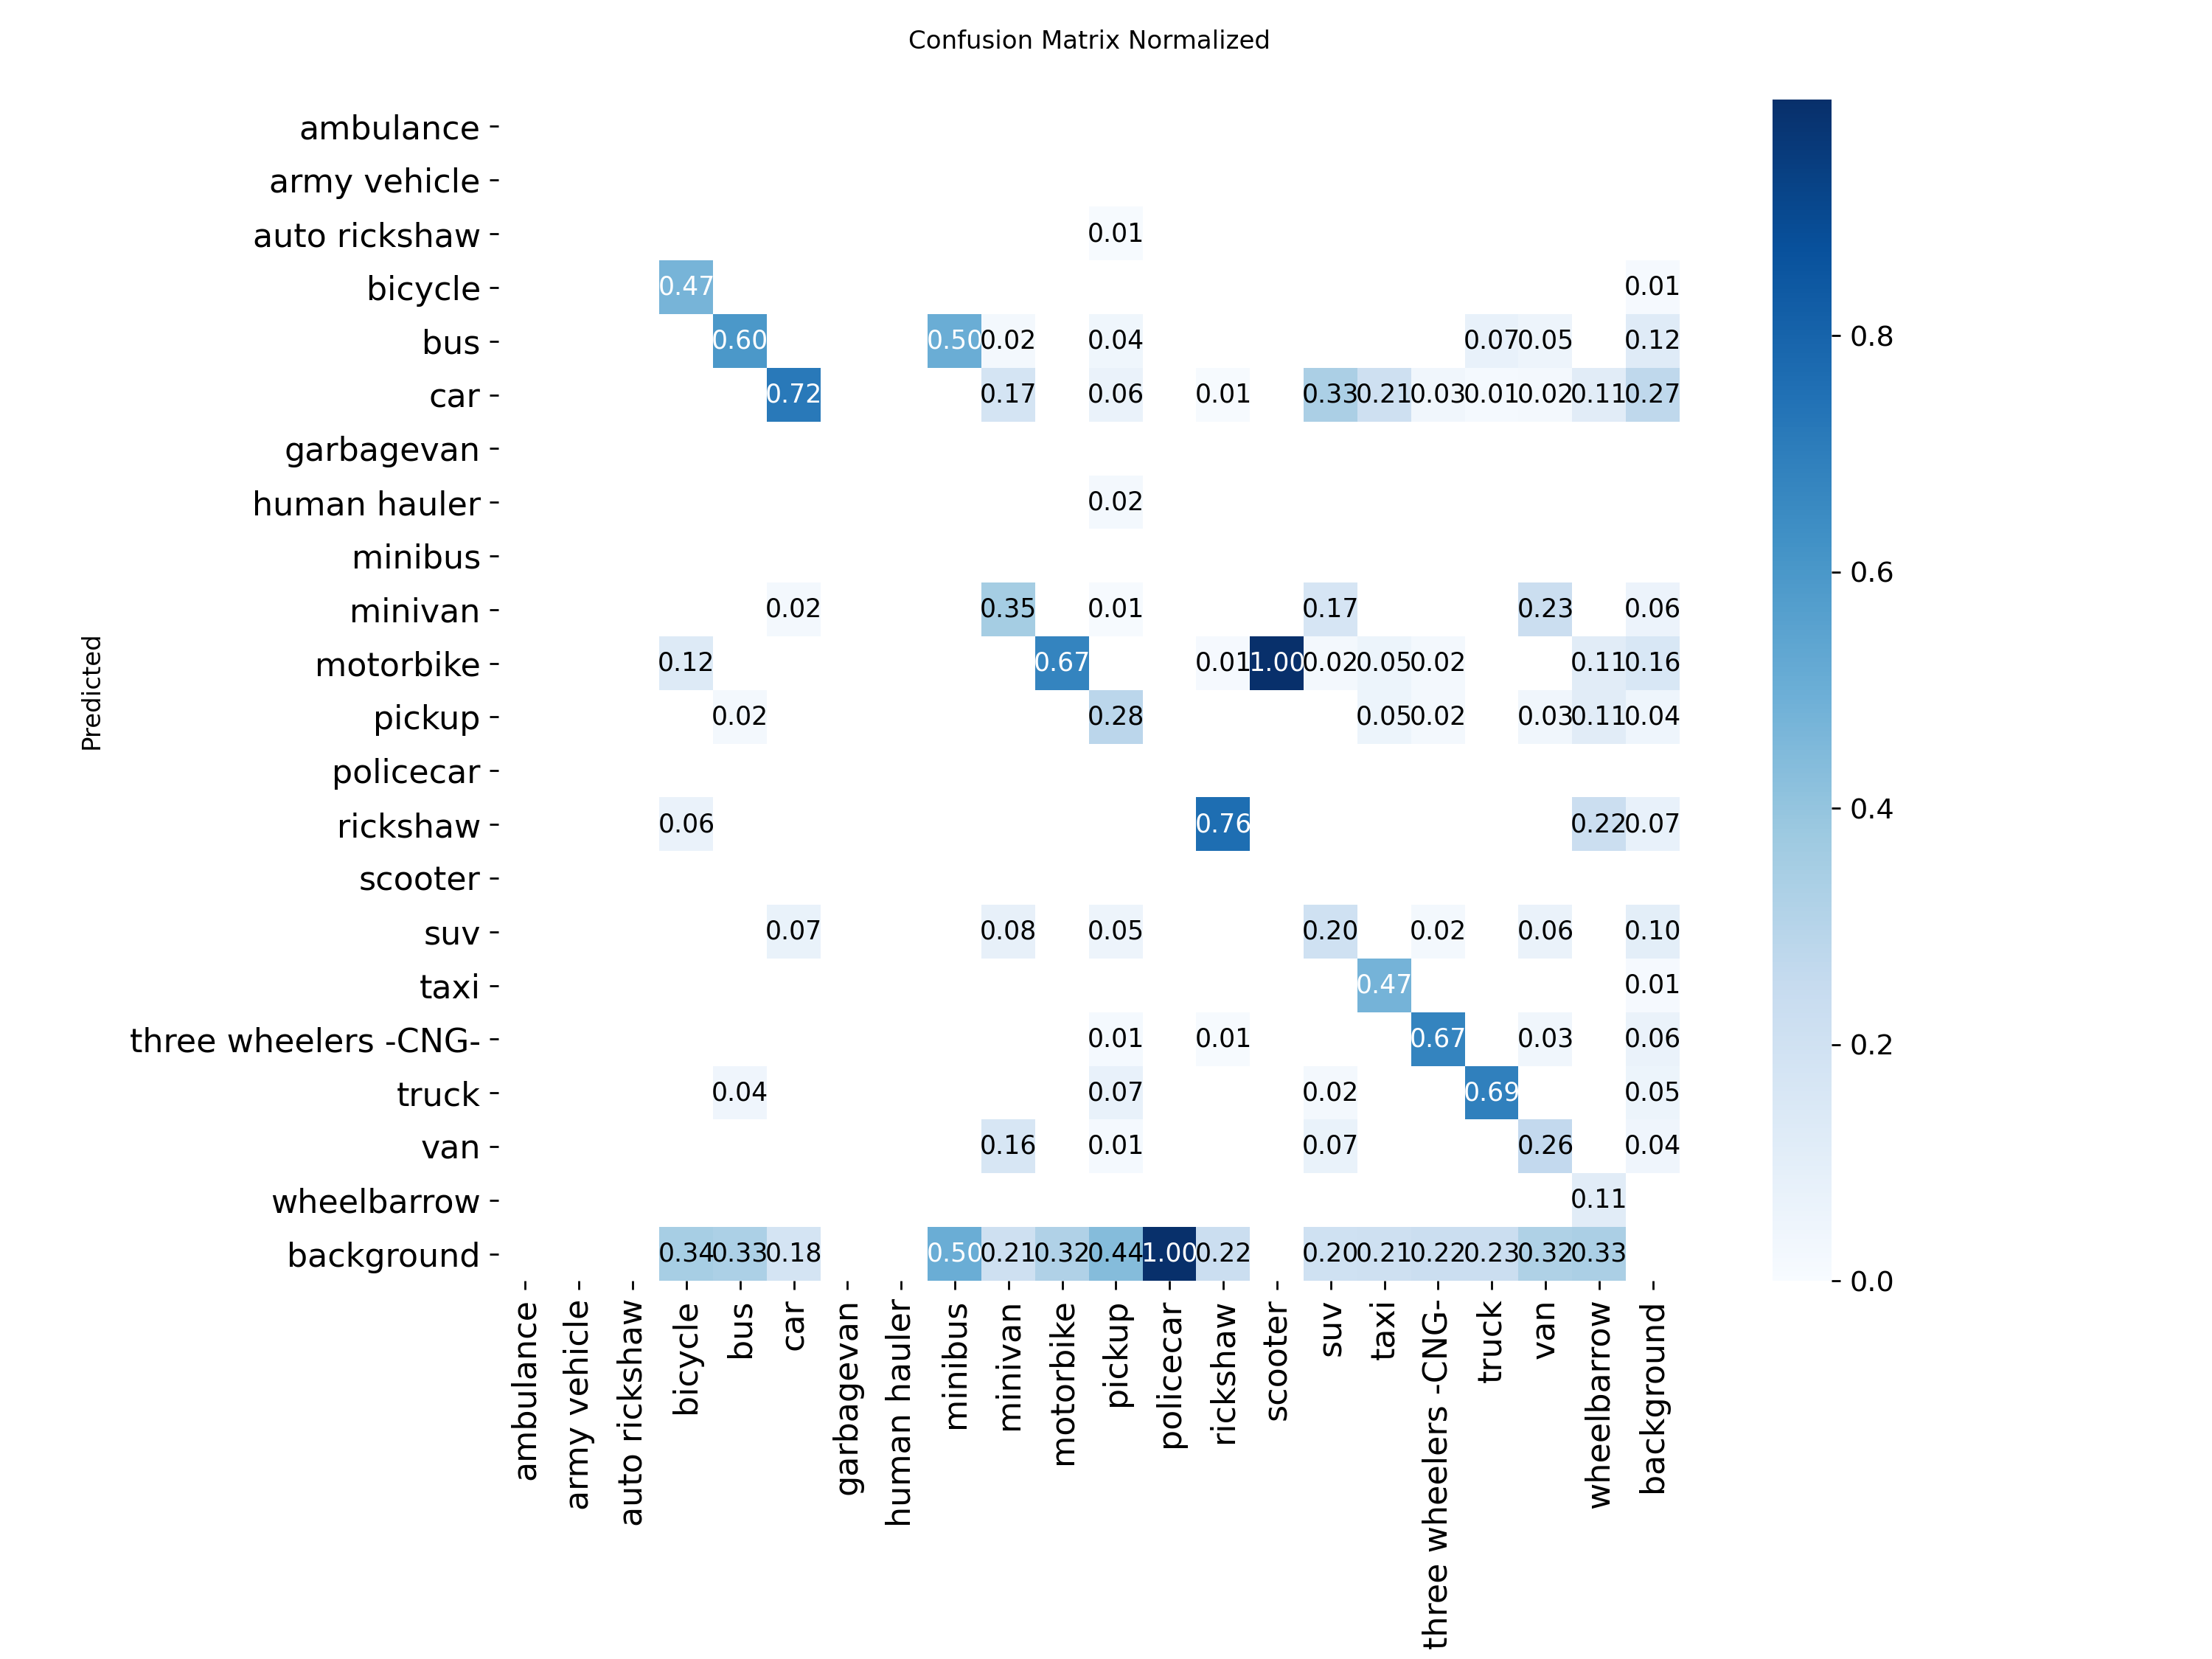
\includegraphics[width=\textwidth]{../tasks/task2_road_vehicle_detection/train_results/confusion_matrix_normalized.png}
        \caption{归一化混淆矩阵}
    \end{subfigure}
    \hfill
    \begin{subfigure}{0.48\textwidth}
        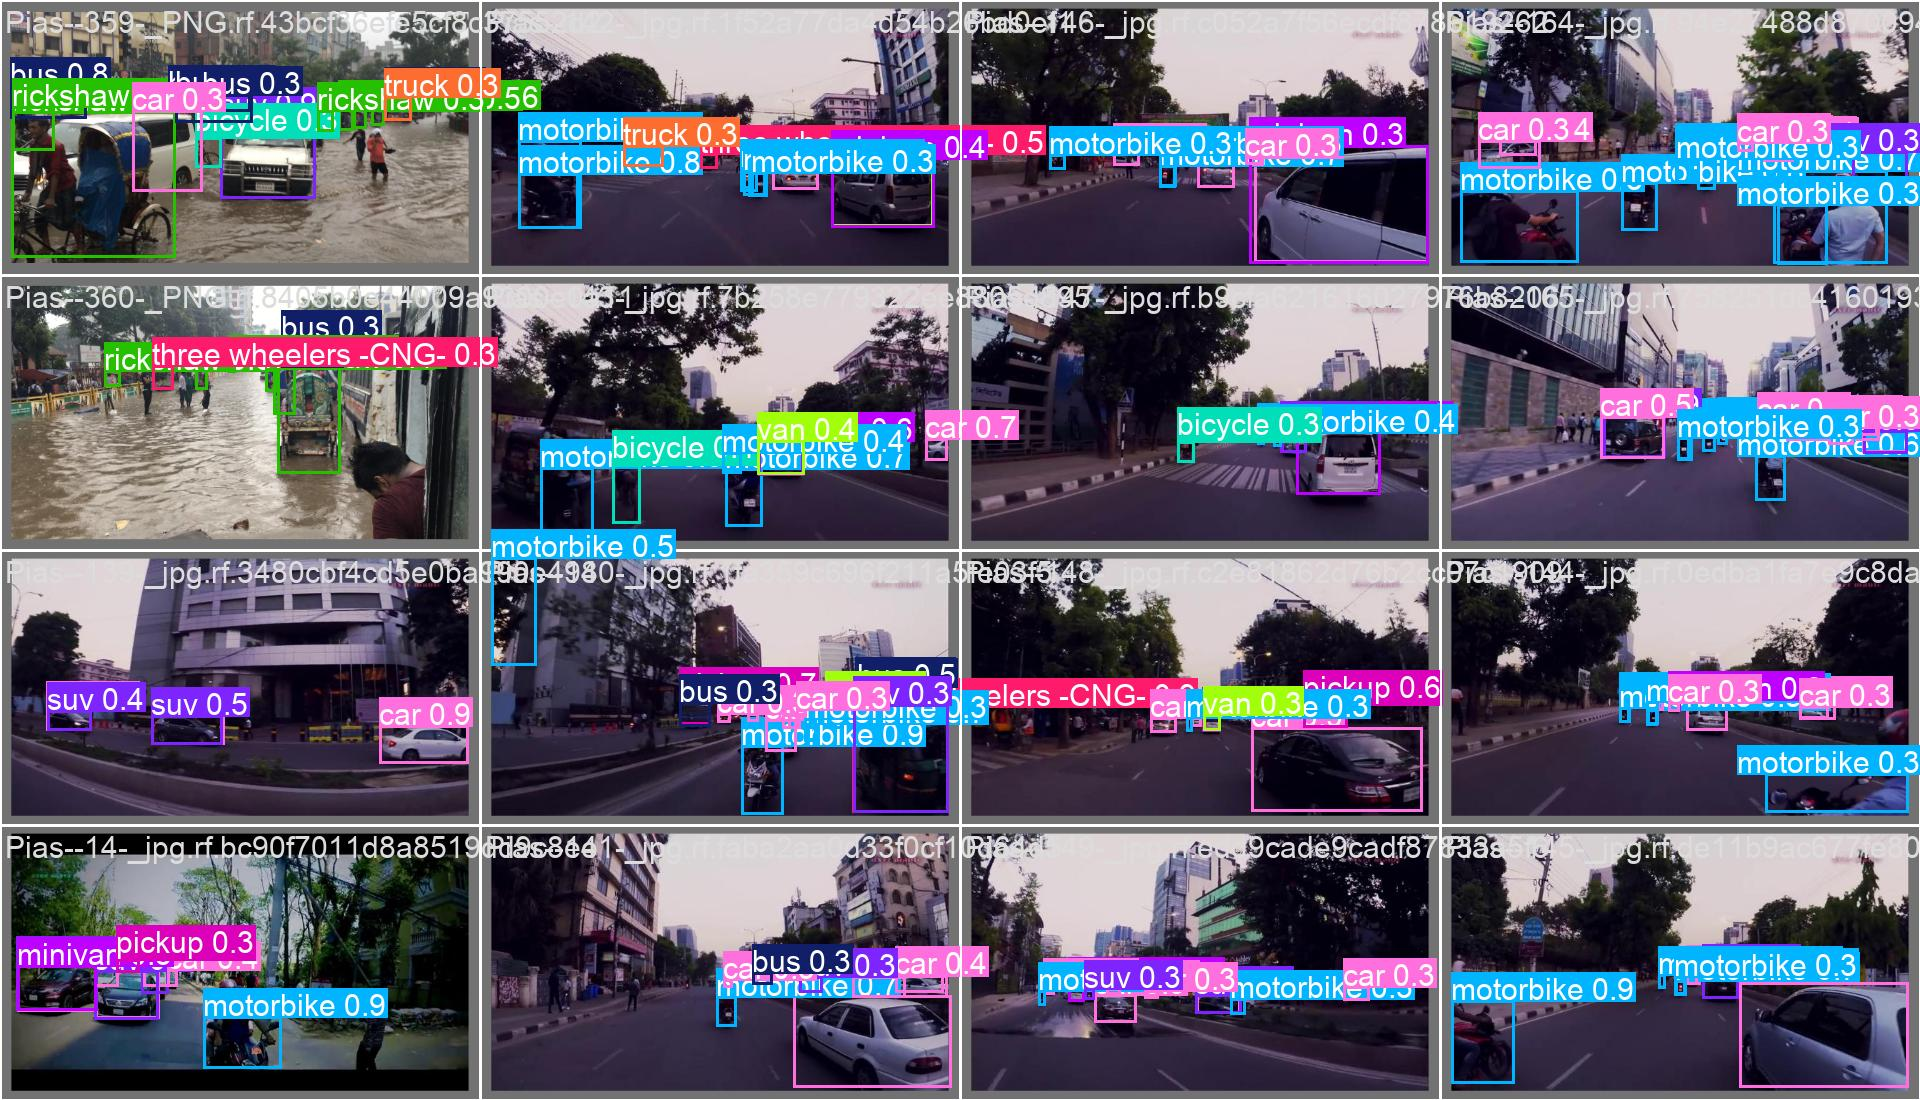
\includegraphics[width=\textwidth]{../tasks/task2_road_vehicle_detection/train_results/val_batch0_pred.jpg}
        \caption{验证集预测样例}
    \end{subfigure}
    \caption{车辆检测类别混淆与预测可视化}
\end{figure}

PR 曲线和 F1 曲线进一步说明，检测器的性能并非由单一置信度阈值决定。对于后续视频跟踪而言，过高的置信度阈值会导致遮挡帧中目标短暂消失，使 tracker 缺少连续观测；过低的阈值则会引入误检，造成错误轨迹。因此，检测模型本身的稳定性和推理阶段阈值选择都会影响最终视频分析效果。混淆矩阵也反映出多类别车辆检测中类别边界并不总是清晰，尤其是尺寸和外观相近的车辆类型更容易发生类别跳变。

\subsection{跟踪计数与遮挡分析}

视频推理阶段对每帧调用 YOLOv8s 检测，并通过 ByteTrack 维持轨迹。ByteTrack 的基本思想是同时利用高置信度和低置信度检测框进行轨迹关联，从而尽量保留被短暂遮挡或置信度下降的目标。实验中推理置信度阈值设为 0.4，IoU 阈值设为 0.4；输出视频在每个目标上绘制 bounding box 与 \code{ID:<track\_id> <class\_name>}，同时绘制画面中线和累计越线数量。

\begin{table}[H]
    \centering
    \caption{跟踪视频与可视化来源}
    \small
    \begin{tabularx}{\textwidth}{llX}
        \toprule
        项目 & 文件或来源 & 说明 \\
        \midrule
        输入视频 & \code{test2.mp4} & 时长约 23.75 s，用于逐帧检测、跟踪和越线计数。 \\
        输出视频 & \code{tracking\_analysis.mp4} & 时长约 23.73 s，为 YOLOv8s + ByteTrack 推理后的可视化结果。 \\
        遮挡关键帧 & \code{frame\_378/424/440.jpg} & 从输出视频中截取，用于分析 ID switch 和类别跳变。 \\
        训练可视化 & Ultralytics plots 与 W\&B & 包括 loss、mAP、PR/F1 曲线、混淆矩阵和验证集预测样例。 \\
        \bottomrule
    \end{tabularx}
\end{table}

越线计数采用轨迹中心点判断。设画面竖直中线为 \(x = W/2\)，每个 track id 保存上一帧中心点横坐标 \(x_{t-1}\) 和当前帧中心点横坐标 \(x_t\)。当满足

\begin{equation}
    x_{t-1} < W/2 \leq x_t
\end{equation}

时，认为该目标从左向右越过计数线。为了避免同一目标重复计数，实验使用已通过 ID 集合保存完成越线的 track id，因此同一条轨迹只会被统计一次。该规则简单直观，适合固定机位道路视频，但它依赖 tracker ID 的连续性；一旦目标在遮挡后被分配新 ID，就可能造成重复计数或漏计。

遮挡分析帧显示：当一辆较大的 SUV 在画面中遮挡较小车辆时，检测框短暂缺失或类别不稳定，ByteTrack 无法可靠延续原轨迹，因此会出现 ID 从 20 切换到 33 的情况；另一个目标保持 ID 22，但类别预测发生跳变。这说明最终跟踪质量不仅取决于 tracker，也强依赖检测器在遮挡场景下的稳定性。

\begin{figure}[H]
    \centering
    \begin{subfigure}{0.32\textwidth}
        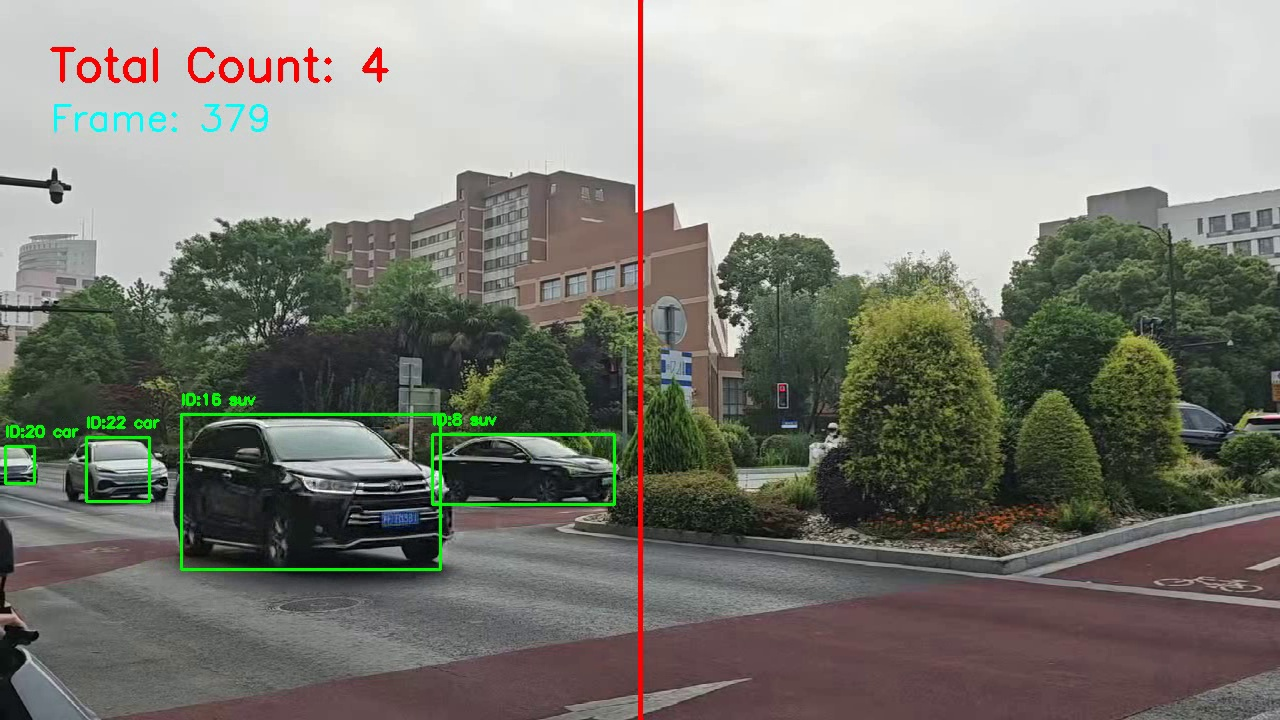
\includegraphics[width=\textwidth]{../tasks/task2_road_vehicle_detection/screenshots/frame_378.jpg}
        \caption{Frame 378}
    \end{subfigure}
    \hfill
    \begin{subfigure}{0.32\textwidth}
        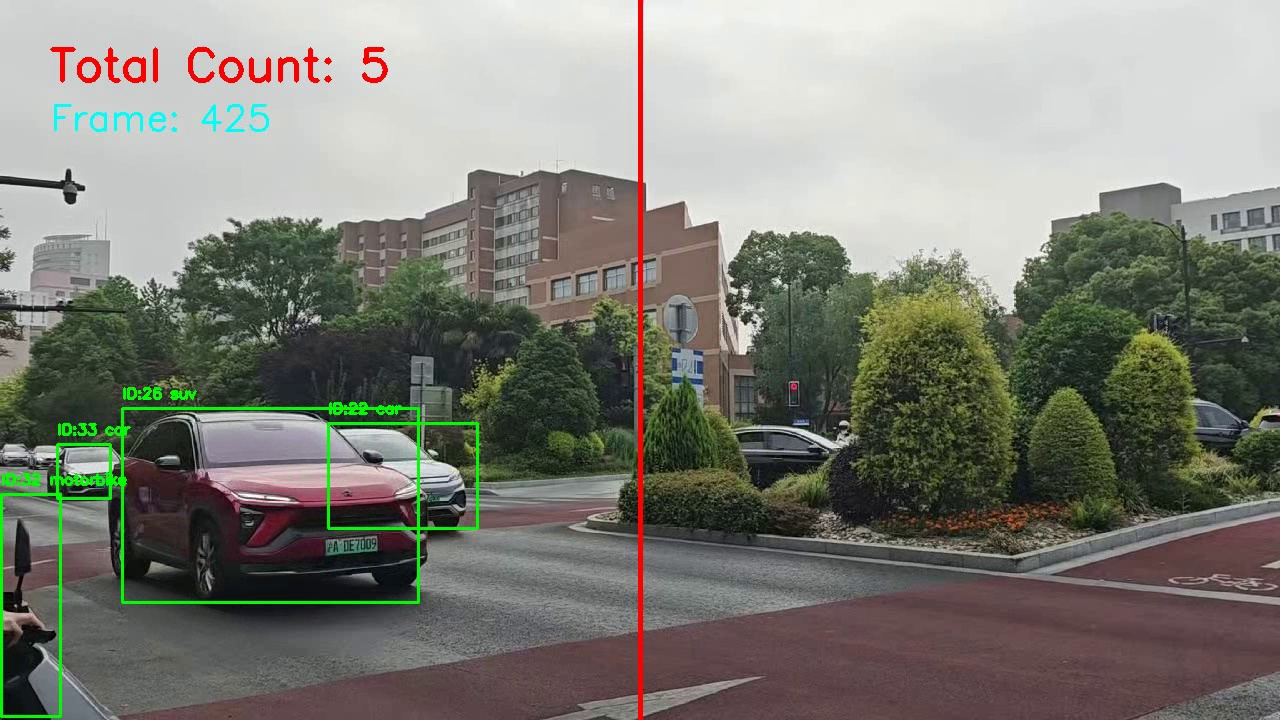
\includegraphics[width=\textwidth]{../tasks/task2_road_vehicle_detection/screenshots/frame_424.jpg}
        \caption{Frame 424}
    \end{subfigure}
    \hfill
    \begin{subfigure}{0.32\textwidth}
        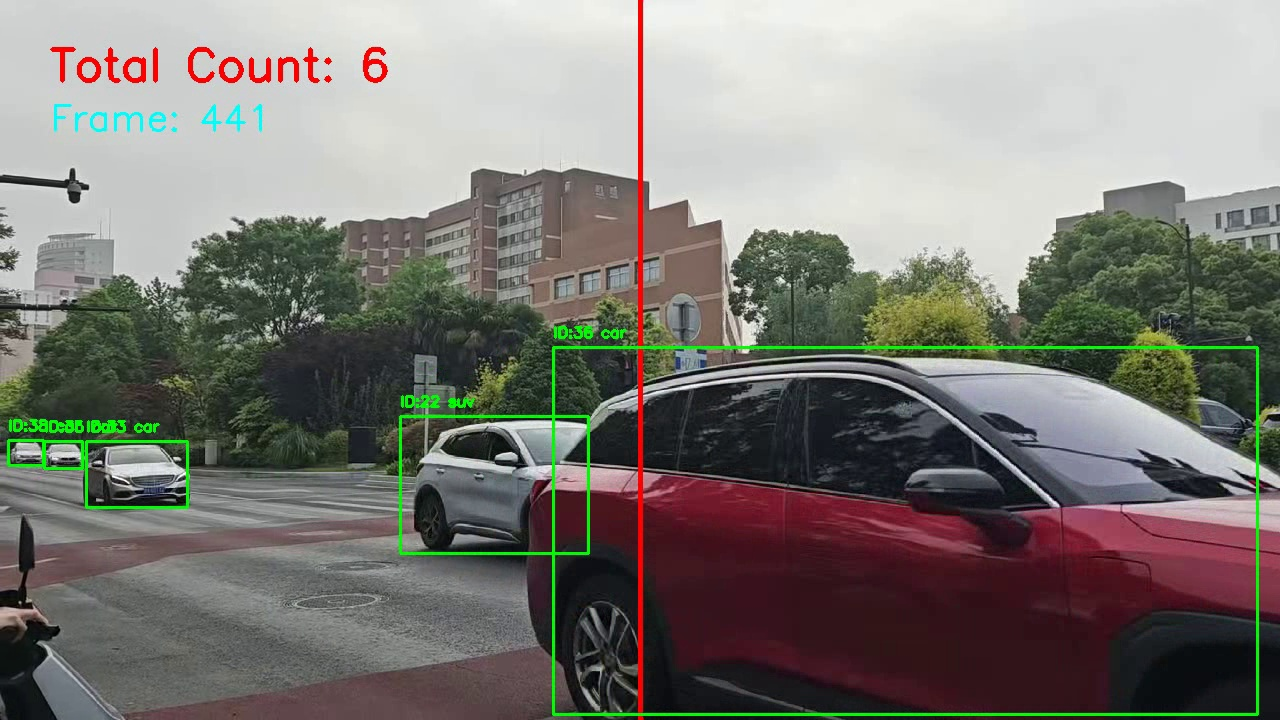
\includegraphics[width=\textwidth]{../tasks/task2_road_vehicle_detection/screenshots/frame_440.jpg}
        \caption{Frame 440}
    \end{subfigure}
    \caption{遮挡导致的 tracking ID 跳变案例}
\end{figure}

从图中可以看到，遮挡发生前目标具有稳定的检测框和 ID：Frame 378 中后方两辆白车分别保持 ID 20 和 ID 22，前景红色 SUV 为 ID 26。到 Frame 424，红色 SUV 与白车发生密集交汇，后方白车被大面积遮挡，原 ID 20 在遮挡后被重新识别为 ID 33，形成 ID switch。Frame 440 中，另一辆白车虽然维持了 ID 22，但类别从 car 瞬时跳变为 suv。

ID 20 跳变的主要原因在于检测缺失和轨迹关联同时失效。ByteTrack 会先根据历史轨迹预测当前位置，再用当前检测框与预测框的 IoU 进行匹配；当目标被 SUV 长时间遮挡时，检测框置信度下降甚至短暂消失，低置信度二次匹配也无法提供可靠观测。同时，后方白车尺度较小并在路口附近存在减速，卡尔曼预测位置与重新出现的检测框之间容易产生偏差，最终导致原轨迹被判定为丢失，新出现的检测框被分配新的 ID。相比之下，ID 22 的遮挡时间较短，重新出现时检测框与预测轨迹仍能匹配，因此保持了原 ID。

类别跳变则更多来自检测器而非 tracker。ByteTrack 主要维护轨迹身份，类别标签仍由每帧 YOLO 检测头给出；当红色 SUV 占据画面主体、白车局部特征被遮挡或被邻近车辆污染时，分类头容易受到干扰。类别级指标也支持这一点：car 的 mAP50 为 0.790，而 suv 只有 0.188，说明模型对 SUV 相关边界的判别更不稳定。该现象说明检测与跟踪并不是两个完全独立的环节：检测器如果在遮挡、远距离和类别相似情况下不稳定，后续轨迹关联就会失去可靠输入。实际系统中可以通过提高检测器召回率、调节 ByteTrack 的匹配阈值、加入运动模型约束或进行摄像机场景标定来缓解该问题。

\section{语义分割实验}

\subsection{数据集与 U-Net 结构}

语义分割实验使用 Stanford Background / ICCV09 风格数据，使用 \code{labels/*.regions.txt} 作为语义标签，共 8 类：sky、tree、road、grass、water、building、mountain、foreground\_object。与图像分类和目标检测不同，语义分割需要为每一个有效像素预测类别，因此模型既要理解全局场景语义，也要恢复局部边界和区域形状。标签中的负数像素表示未知区域，训练时统一映射为 \code{ignore\_index = 255}，损失和指标计算时忽略这些像素，避免未知标注干扰模型学习。

图 \ref{fig:segmentation-dataset-example} 给出了输入图像与语义标签样例。标签不再使用检测任务中的矩形框，而是为每个有效像素分配语义类别；同一幅图像中同时包含天空、树木、道路、建筑和前景目标等区域。可以看到，天空、建筑、道路等大面积类别在像素数量上占据主导，而 foreground\_object 等小区域面积很小，边界也更容易受分辨率和下采样影响。因此，分割实验不能只依赖 pixel accuracy，还需要使用 mIoU 和 per-class IoU 衡量小类别和区域边界的恢复质量。

\begin{figure}[htbp]
    \centering
    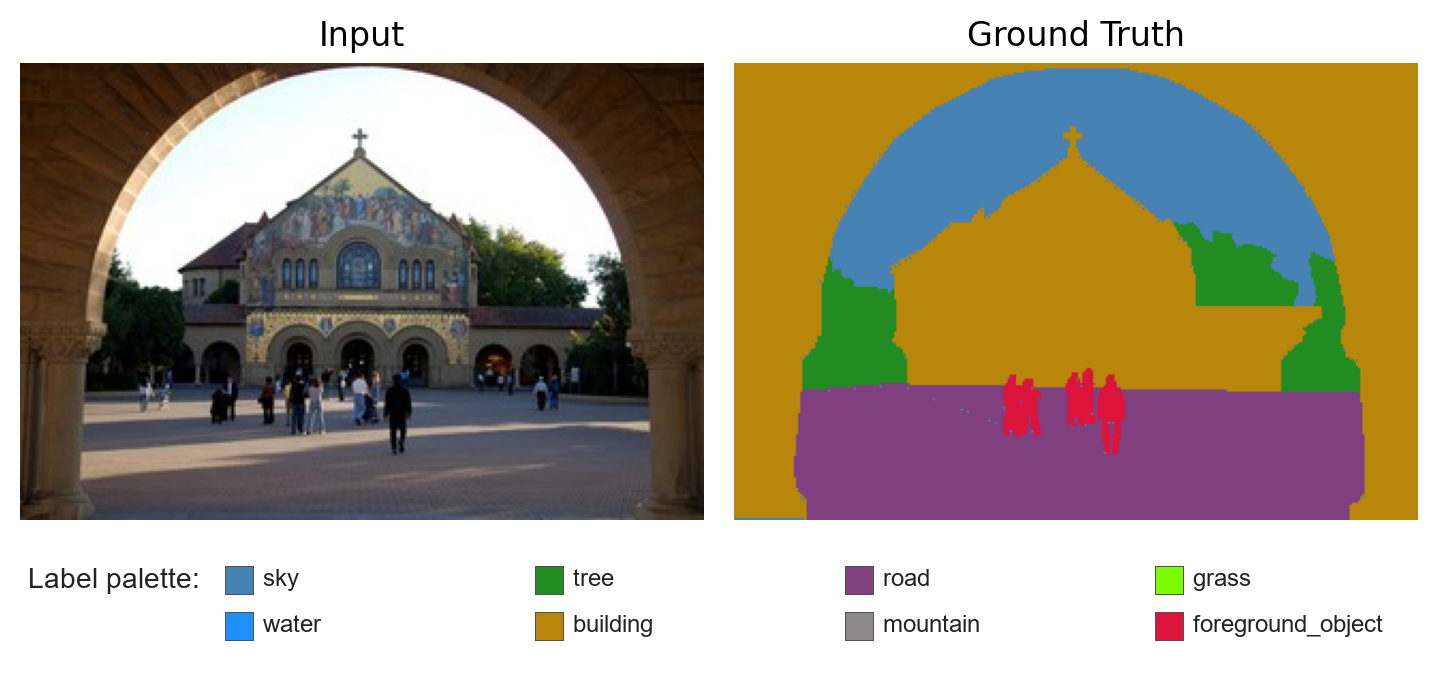
\includegraphics[width=0.88\textwidth]{../tasks/task3_semantic_segmentation/report_figures/segmentation_dataset_label_example.png}
    \caption{Stanford Background / ICCV09 风格语义标签样例}
    \label{fig:segmentation-dataset-example}
\end{figure}

模型采用手写轻量 U-Net，包括编码器下采样、瓶颈层特征提取、解码器上采样、skip connection 和最终 \code{1x1 Conv} 像素分类头。编码器每一级使用两个 \(3\times3\) 卷积、BatchNorm 和 ReLU 组成的 ConvBlock，并通过 max pooling 降低空间分辨率；解码器使用转置卷积逐级上采样，并与对应编码层特征拼接。U-Net 的 skip connection 能将浅层空间细节直接传递到解码阶段，适合语义分割中边界和局部区域恢复。

\begin{table}[H]
    \centering
    \caption{轻量 U-Net 结构}
    \small
    \begin{tabular}{lll}
        \toprule
        模块 & 空间操作 & 通道数 \\
        \midrule
        Encoder 1 & ConvBlock & 32 \\
        Encoder 2 & MaxPool + ConvBlock & 64 \\
        Encoder 3 & MaxPool + ConvBlock & 128 \\
        Encoder 4 & MaxPool + ConvBlock & 256 \\
        Bottleneck & MaxPool + ConvBlock & 512 \\
        Decoder & Transposed Conv + skip connection & 256, 128, 64, 32 \\
        Head & \(1\times1\) Conv & 8 classes \\
        \bottomrule
    \end{tabular}
\end{table}

\begin{table}[H]
    \centering
    \caption{语义分割训练配置}
    \small
    \begin{tabular}{ll}
        \toprule
        Setting & Value \\
        \midrule
        Model & U-Net \\
        Input size & \(256 \times 256\) \\
        Epochs & 100 \\
        Batch size & 8 \\
        Learning rate & \(3\times10^{-4}\) \\
        Optimizer & AdamW \\
        Weight decay & \(1\times10^{-4}\) \\
        Seed & 42 \\
        \bottomrule
    \end{tabular}
\end{table}

\subsection{损失函数设计}

实验比较三种损失函数配置：

\begin{itemize}
    \item Cross-Entropy Loss：逐像素多分类监督，训练稳定；
    \item 手写 Soft Dice Loss：直接优化预测区域与真实区域的重叠程度；
    \item Cross-Entropy + Dice：兼顾像素级分类稳定性与区域级重叠优化。
\end{itemize}

交叉熵损失对每一个有效像素进行多分类监督，其形式为

\begin{equation}
    \mathcal{L}_{CE} = - \frac{1}{|\Omega|}\sum_{i \in \Omega}\log p_{i,y_i},
\end{equation}

其中 \(\Omega\) 表示非忽略像素集合，\(y_i\) 为像素 \(i\) 的真实类别，\(p_{i,y_i}\) 为模型对真实类别的预测概率。交叉熵训练稳定，能够直接优化逐像素分类正确率，但当类别面积差异较大时，大面积类别会在损失中占据更高权重。

Dice 系数直接衡量预测区域和真实区域的重叠程度。实验中手写实现多类别 Soft Dice Loss：先对 logits 做 softmax，再将标签转换为 one-hot 表示，并用 \code{ignore\_index} mask 去除未知像素。对第 \(c\) 类，Dice 系数为

\begin{equation}
    Dice_c = \frac{2\sum_i p_{i,c}g_{i,c} + \epsilon}{\sum_i p_{i,c} + \sum_i g_{i,c} + \epsilon},
\end{equation}

最终损失为 \(1-\frac{1}{C}\sum_c Dice_c\)。由于 Dice Loss 直接优化预测区域和真实区域的重叠程度，它通常比单纯逐像素交叉熵更关注区域级覆盖质量，尤其适合类别不均衡或小区域类别较多的分割场景。组合损失使用 \(\mathcal{L}_{CE}+\mathcal{L}_{Dice}\)，希望同时保留交叉熵的分类稳定性和 Dice 的区域重叠优化能力。

\subsection{分割结果}

三种损失函数在验证集上的结果如表 \ref{tab:segmentation-loss-results} 所示。Dice Loss 在验证集 mIoU 上最高，说明直接优化区域重叠对该数据集更有帮助；CE+Dice 的 pixel accuracy 最高，但 mIoU 略低于纯 Dice，说明它对大面积类别更稳定，而对小类区域的重叠优化略弱。单独使用 Cross-Entropy 的 pixel accuracy 与另外两组接近，但 mIoU 明显偏低，说明只看像素准确率会掩盖类别不均衡带来的问题。

\begin{table}[H]
    \centering
    \caption{三种损失函数验证集结果}
    \label{tab:segmentation-loss-results}
    \small
    \begin{tabular}{lrrr}
        \toprule
        Loss & Best epoch & Best Val mIoU & Best Val Pixel Acc. \\
        \midrule
        Cross-Entropy & 90 & 0.2587 & 0.7667 \\
        Dice & 72 & 0.3055 & 0.7671 \\
        Cross-Entropy + Dice & 90 & 0.3027 & 0.7748 \\
        \bottomrule
    \end{tabular}
\end{table}

\subsubsection{单组训练曲线分析}

除总体对比曲线外，每一种损失函数的单独训练过程也能反映不同优化目标的特点。图 \ref{fig:segmentation-ce-curves} 展示了 Cross-Entropy 的训练曲线。该组实验的训练 loss 持续下降，训练 mIoU 在后期升至 0.40 左右，但验证 mIoU 在 0.23--0.26 附近波动，最佳验证 mIoU 为 0.2587，出现在第 90 个 epoch。与此同时，验证 loss 在第 40 个 epoch 左右已经达到较低值，之后反而上升。这说明模型继续拟合训练集时，验证集区域重叠质量并没有同步提升；交叉熵更直接优化逐像素分类概率，容易在大面积类别上取得较高像素准确率，但对小区域类别和类别边界的 mIoU 提升有限。

\begin{figure}[H]
    \centering
    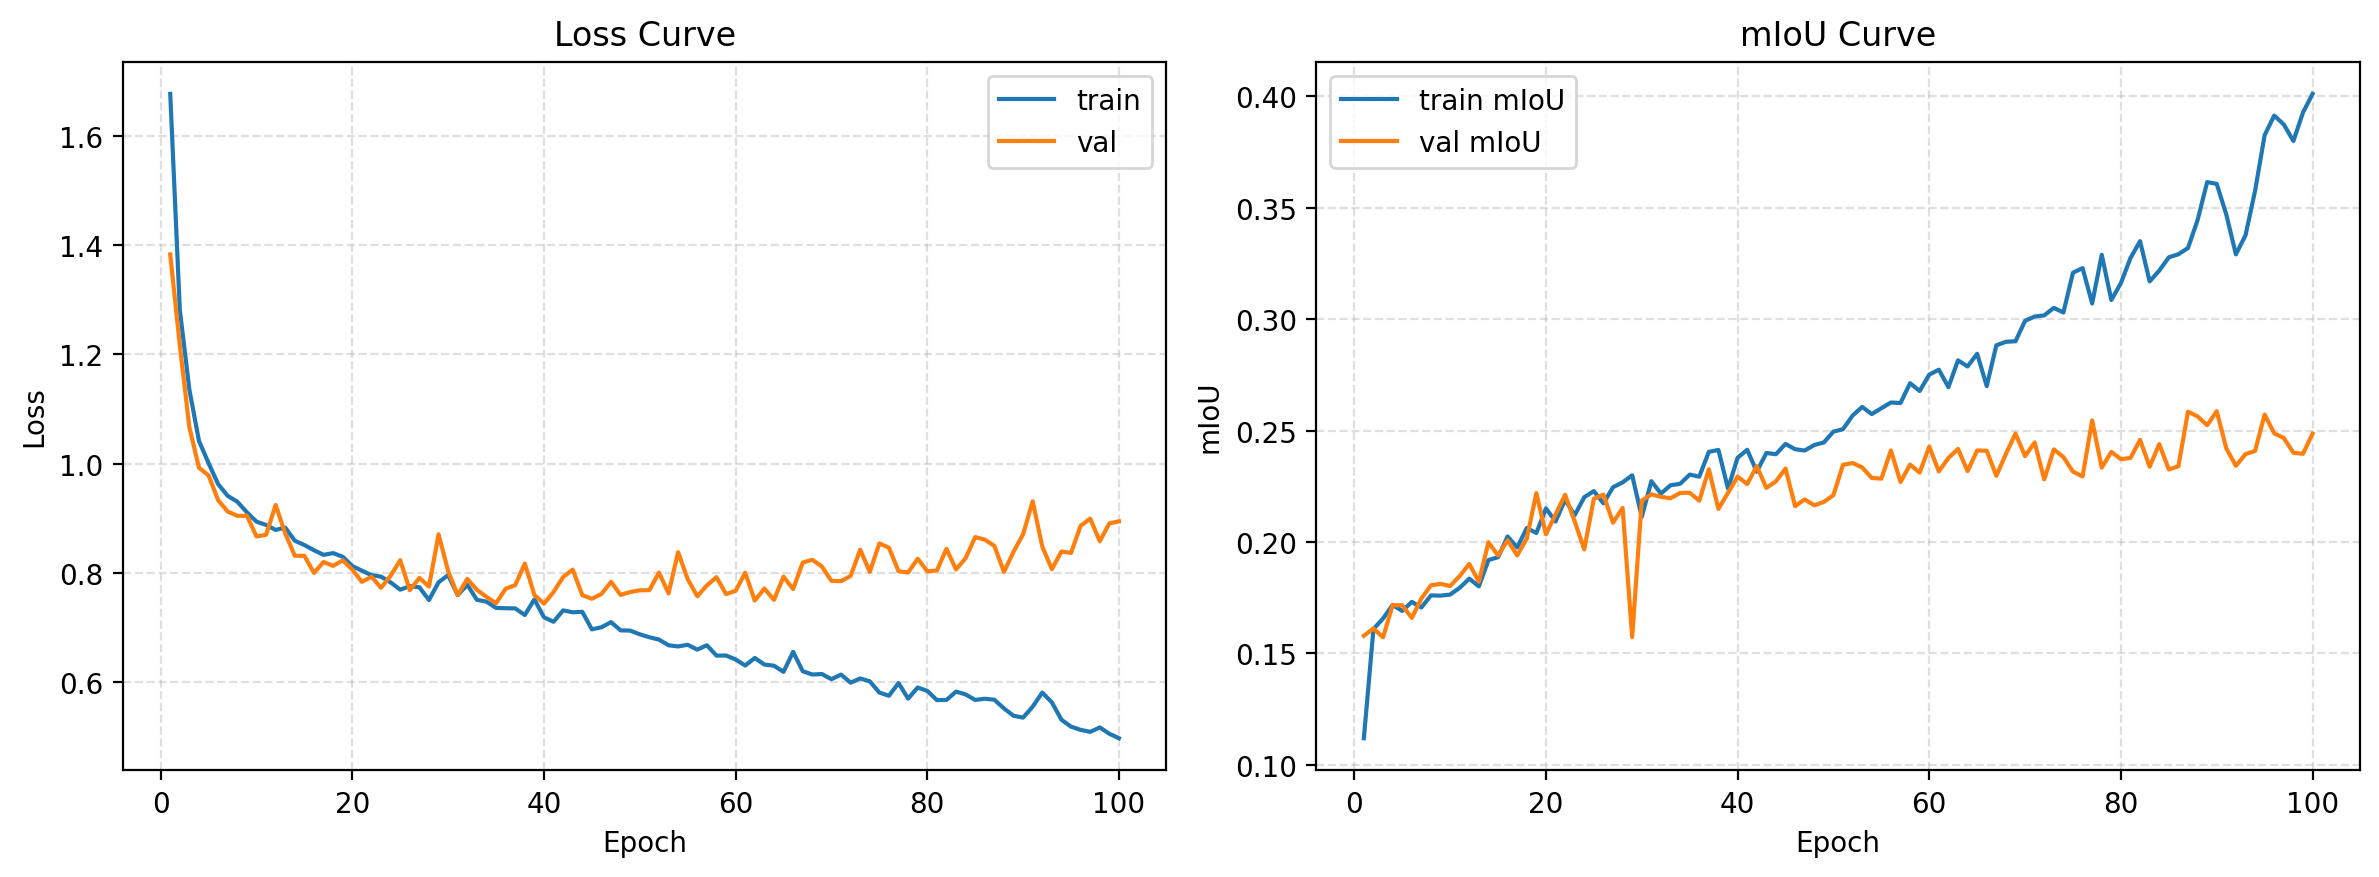
\includegraphics[width=0.86\textwidth]{../tasks/task3_semantic_segmentation/runs/loss_comparison/ce/training_curves.png}
    \caption{Cross-Entropy 单组训练曲线}
    \label{fig:segmentation-ce-curves}
\end{figure}

图 \ref{fig:segmentation-dice-curves} 展示了 Dice Loss 的训练过程。Dice Loss 的验证 mIoU 在中期持续上升，并在第 72 个 epoch 达到 0.3055，是三组实验中最高的 mIoU。后期验证 loss 仍有下降，但验证 mIoU 下降到 0.25 左右，说明 Soft Dice 损失值与最终硬标签 mIoU 并不完全单调一致，模型选择时仍需要以验证 mIoU 作为主要依据。与 Cross-Entropy 相比，Dice Loss 明显提升了 tree、road、grass、building 和 foreground\_object 等类别的 IoU，说明直接优化区域重叠有助于缓解像素面积不均衡。

\begin{figure}[H]
    \centering
    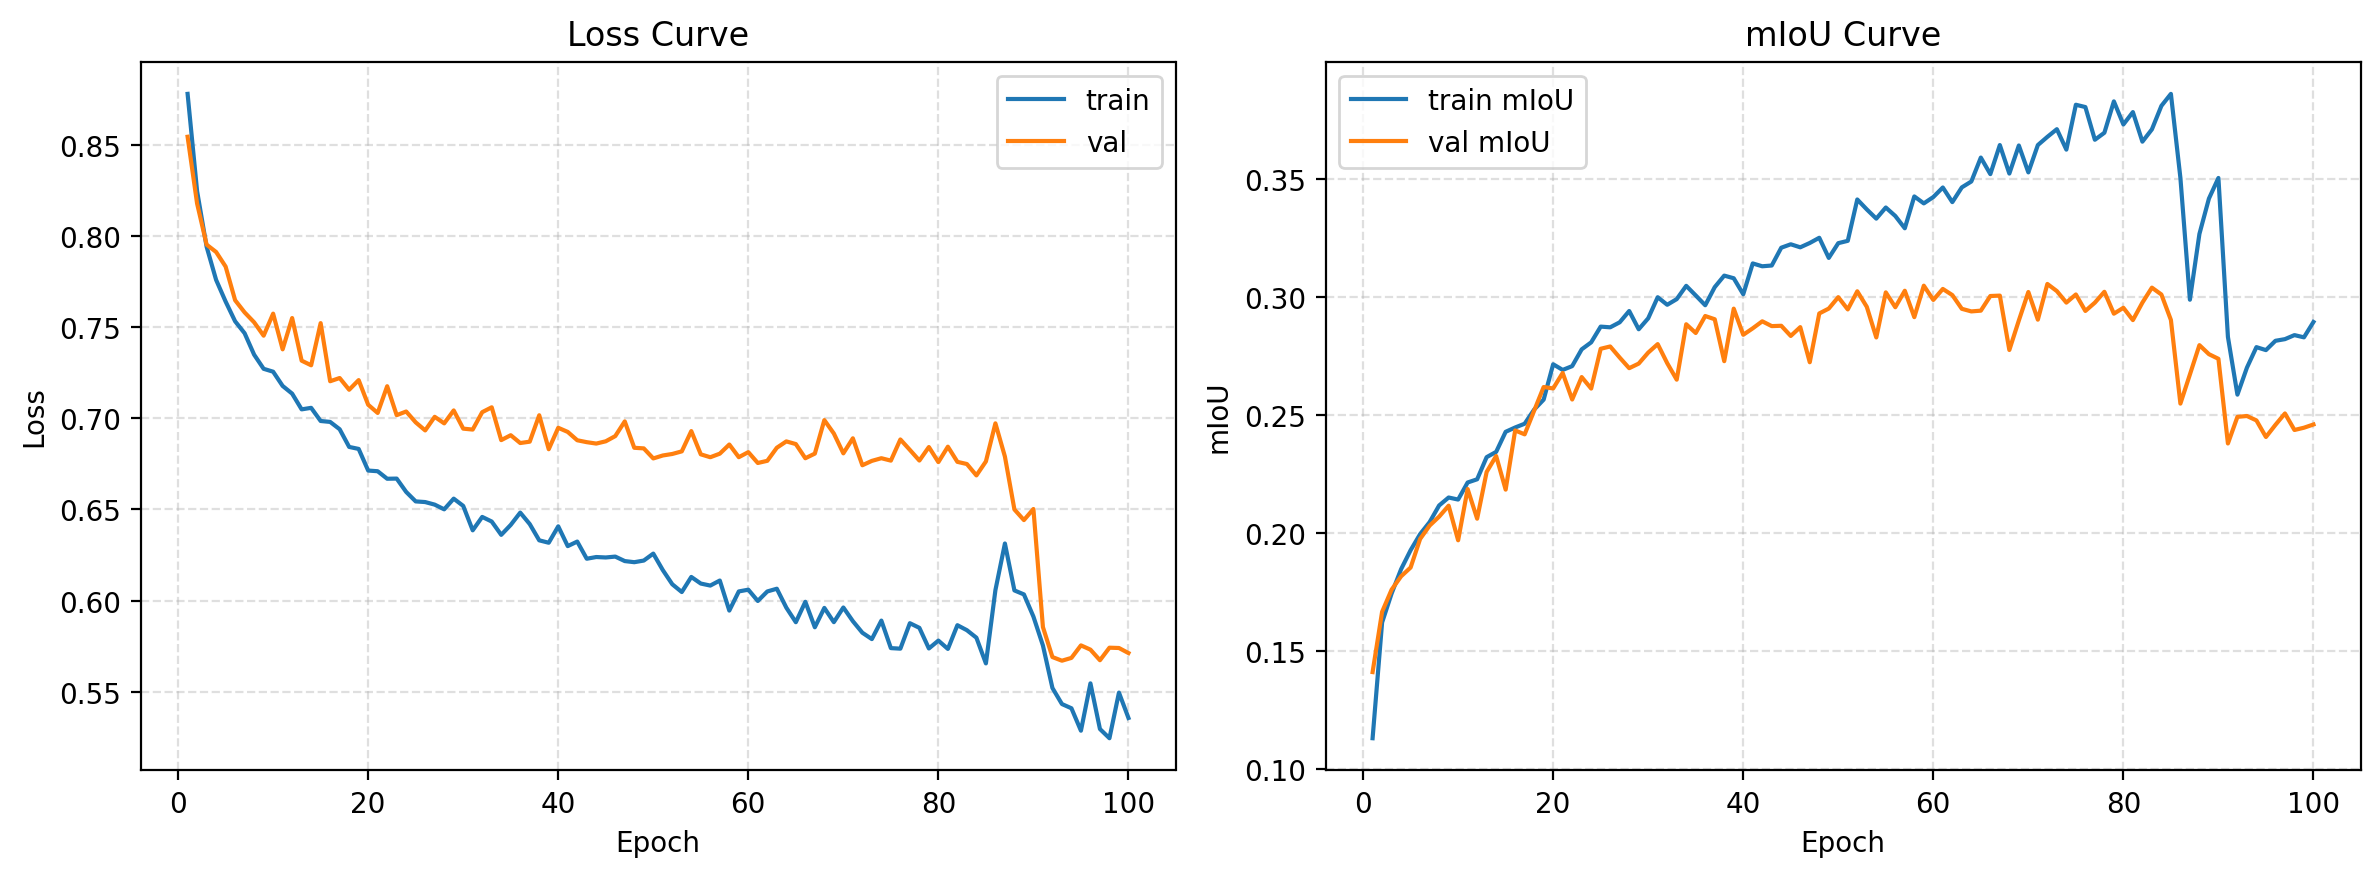
\includegraphics[width=0.86\textwidth]{../tasks/task3_semantic_segmentation/runs/loss_comparison/dice/training_curves.png}
    \caption{Dice Loss 单组训练曲线}
    \label{fig:segmentation-dice-curves}
\end{figure}

图 \ref{fig:segmentation-combo-curves} 展示了 Cross-Entropy + Dice 的训练过程。组合损失的训练 mIoU 上升最快，最终训练 mIoU 接近 0.49，验证集最佳 mIoU 为 0.3027，略低于纯 Dice，但 pixel accuracy 最高，达到 0.7748。该结果说明组合损失确实增强了整体像素分类稳定性，尤其对大面积区域更友好；但当 CE 与 Dice 简单等权相加时，交叉熵项仍会把一部分优化重心拉回高频像素类别，因此 mIoU 没有超过纯 Dice。后期训练曲线还显示出训练集和验证集之间的差距，说明该轻量 U-Net 在 100 个 epoch 内已经出现一定过拟合。

\begin{figure}[H]
    \centering
    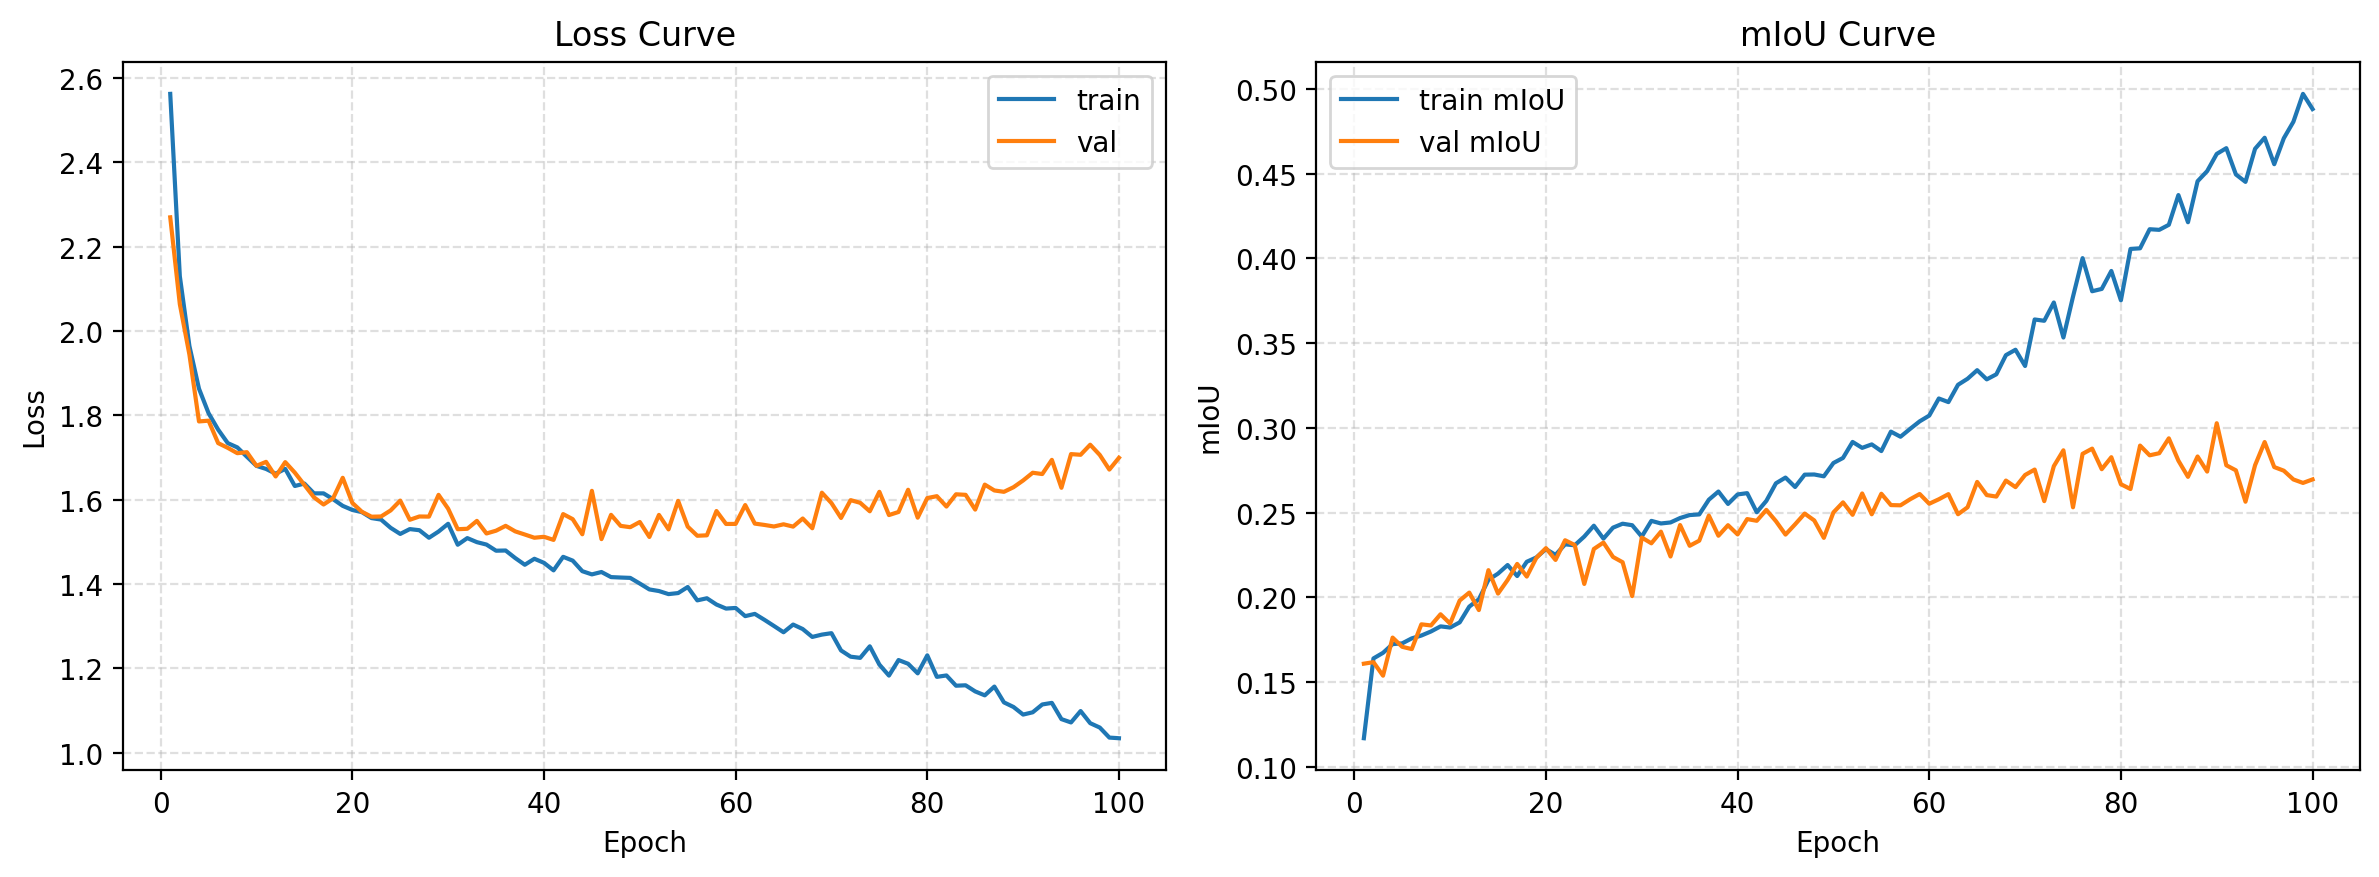
\includegraphics[width=0.86\textwidth]{../tasks/task3_semantic_segmentation/runs/loss_comparison/combo/training_curves.png}
    \caption{Cross-Entropy + Dice 单组训练曲线}
    \label{fig:segmentation-combo-curves}
\end{figure}

为了进一步分析不同损失函数对各类别的影响，表 \ref{tab:segmentation-per-class-iou} 给出了验证集 per-class IoU。Cross-Entropy 在 sky 上表现很好，但 road 的 IoU 为 0，说明模型几乎没有学到该类别的有效区域；Dice Loss 显著提升 tree、road、grass、building 和 foreground\_object 等类别的 IoU，因此 mIoU 最高。CE+Dice 在 sky、grass、water 和 mountain 上较强，并取得最高 pixel accuracy，但 tree、road 和 building 的平均表现略弱于纯 Dice，因此总体 mIoU 略低。

\begin{table}[H]
    \centering
    \caption{三种损失函数的 per-class IoU}
    \label{tab:segmentation-per-class-iou}
    \small
    \begin{tabular}{lccc}
        \toprule
        类别 & Cross-Entropy & Dice & \shortstack{Cross-Entropy\\+ Dice} \\
        \midrule
        sky & 0.8540 & 0.8452 & 0.8597 \\
        tree & 0.2010 & 0.3686 & 0.3020 \\
        road & 0.0000 & 0.2163 & 0.1658 \\
        grass & 0.1622 & 0.2070 & 0.2099 \\
        water & 0.1190 & 0.0626 & 0.1541 \\
        building & 0.4399 & 0.4585 & 0.4349 \\
        mountain & 0.1164 & 0.0793 & 0.1184 \\
        foreground\_object & 0.1769 & 0.2060 & 0.1768 \\
        \bottomrule
    \end{tabular}
\end{table}

\begin{figure}[H]
    \centering
    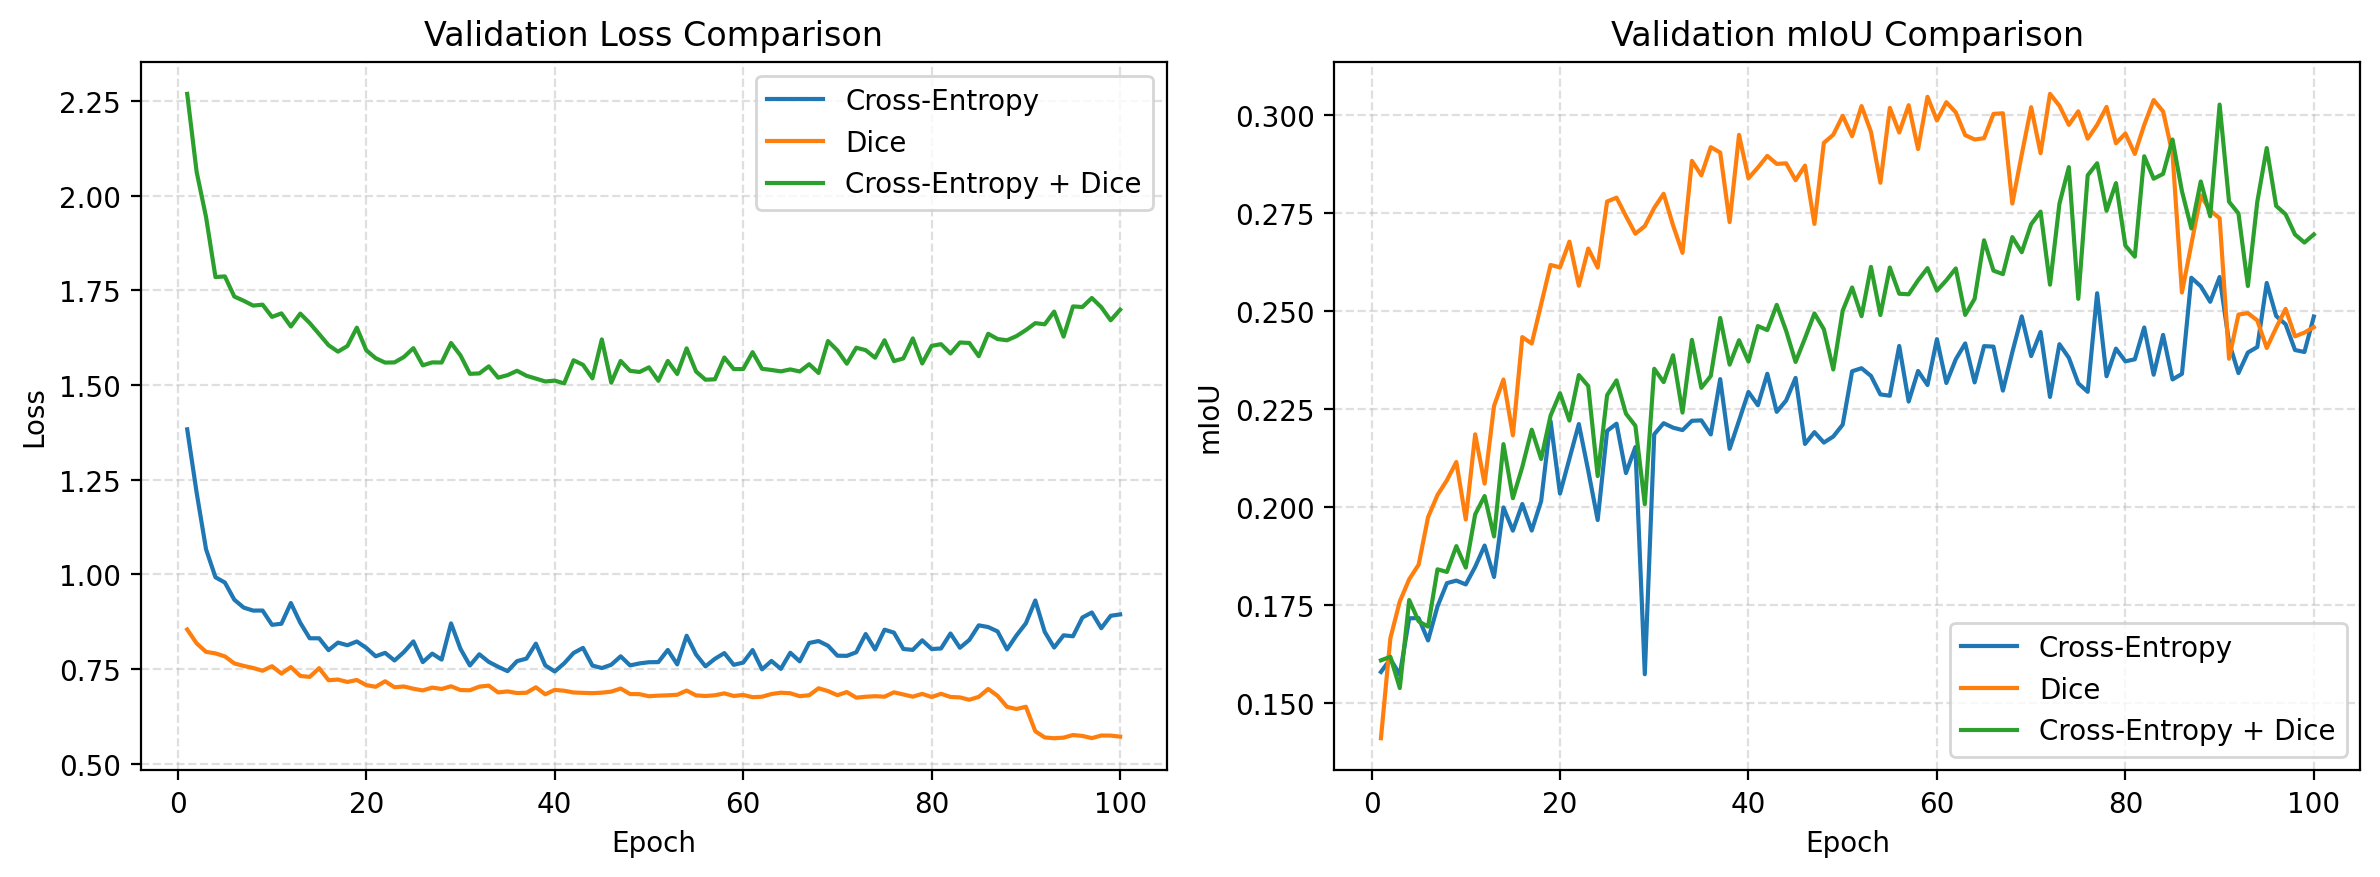
\includegraphics[width=0.92\textwidth]{../tasks/task3_semantic_segmentation/runs/loss_comparison/miou_loss_comparison.png}
    \caption{三种损失函数的 mIoU 与 loss 对比}
\end{figure}

\begin{figure}[H]
    \centering
    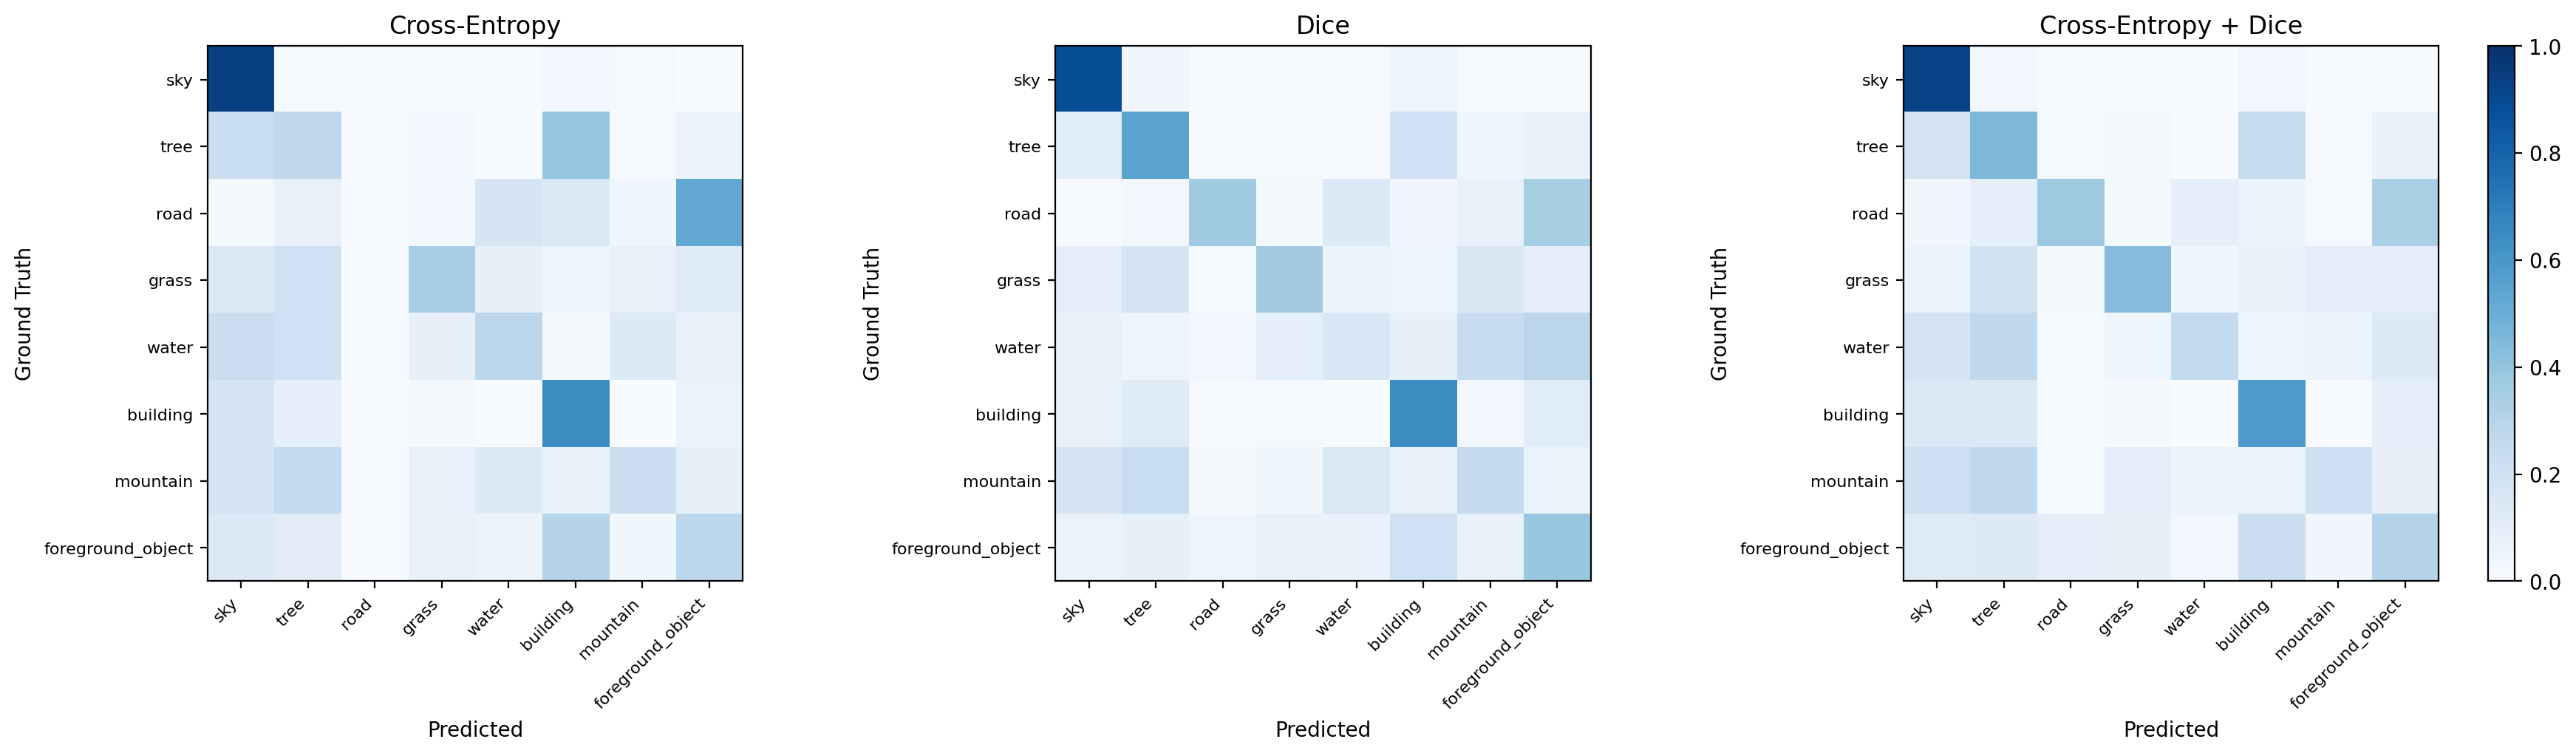
\includegraphics[width=0.92\textwidth]{../tasks/task3_semantic_segmentation/runs/loss_comparison/confusion_matrix_comparison.png}
    \caption{三种损失函数的混淆矩阵对比}
\end{figure}

\begin{figure}[H]
    \centering
    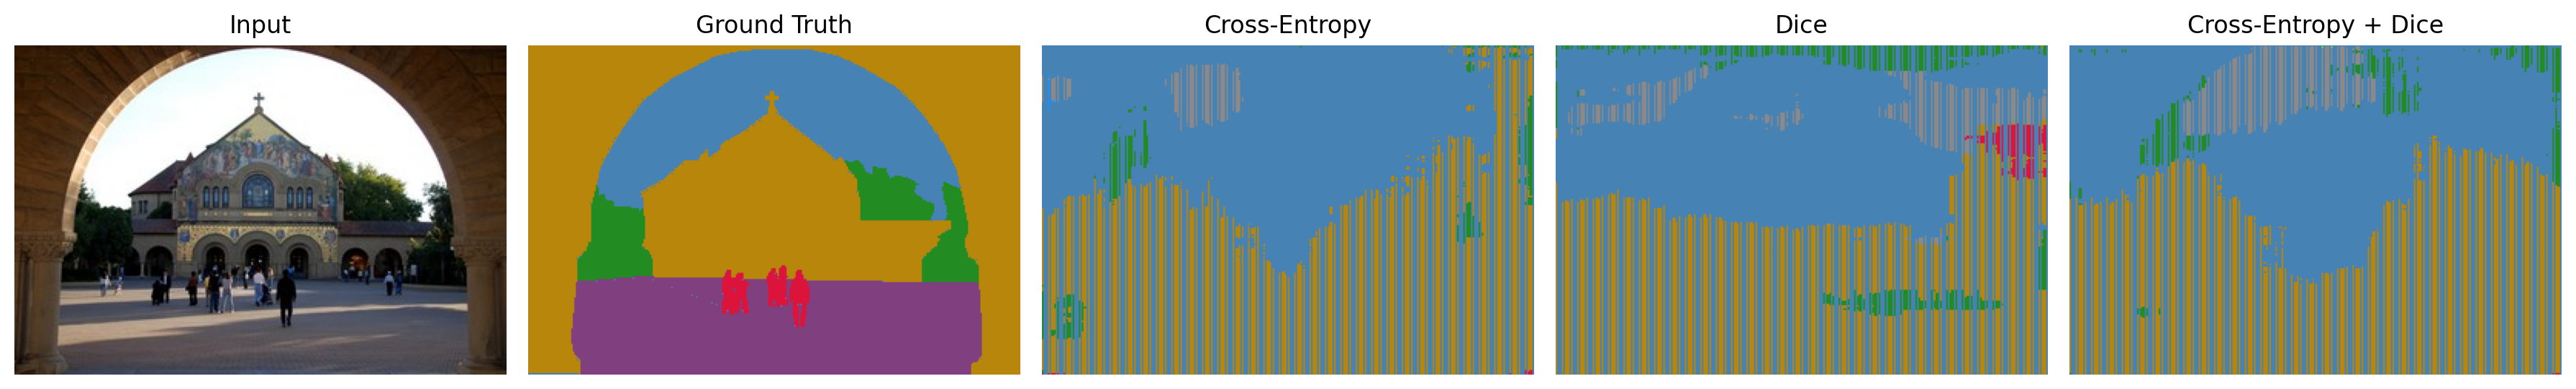
\includegraphics[width=0.96\textwidth]{../tasks/task3_semantic_segmentation/runs/loss_comparison/0000382_prediction_comparison.png}
    \caption{样例预测对比}
\end{figure}

分割实验的可视化来源为三组损失函数训练后的 history、混淆矩阵和样例预测输出，并由统一对比脚本汇总生成。这样可以同时观察数值曲线、类别混淆和具体图像上的区域恢复效果，避免只根据单张预测图判断损失函数优劣。

曲线对比显示，Dice Loss 在中后期达到最高 mIoU，但其训练过程并非始终在 pixel accuracy 上占优；CE+Dice 的 pixel accuracy 最高，说明组合损失更容易提高大面积区域的逐像素分类正确率。混淆矩阵进一步显示，sky 和 building 是相对稳定的类别，而 road、water、mountain 等类别更容易与周围场景混淆。

\subsubsection{样例预测分析}

图 \ref{fig:segmentation-single-predictions} 单独列出了样本 \code{0000382} 在三种损失函数下的预测结果。该样本同时包含天空、建筑、道路/地面、树木和前景行人，能够较直观地观察模型对大面积区域和小目标区域的处理差异。

\begin{figure}[H]
    \centering
    \begin{subfigure}{0.31\textwidth}
        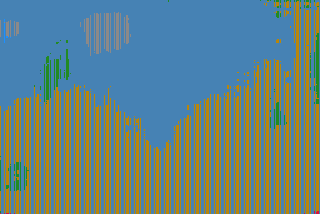
\includegraphics[width=\textwidth]{../tasks/task3_semantic_segmentation/runs/loss_comparison/0000382_ce.png}
        \caption{Cross-Entropy}
    \end{subfigure}
    \hfill
    \begin{subfigure}{0.31\textwidth}
        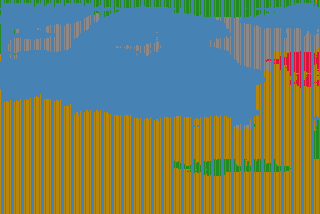
\includegraphics[width=\textwidth]{../tasks/task3_semantic_segmentation/runs/loss_comparison/0000382_dice.png}
        \caption{Dice}
    \end{subfigure}
    \hfill
    \begin{subfigure}{0.31\textwidth}
        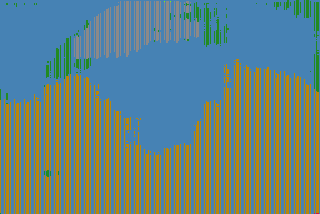
\includegraphics[width=\textwidth]{../tasks/task3_semantic_segmentation/runs/loss_comparison/0000382_combo.png}
        \caption{Cross-Entropy + Dice}
    \end{subfigure}
    \caption{样例预测的单组结果}
    \label{fig:segmentation-single-predictions}
\end{figure}

Cross-Entropy 的预测更容易偏向主导类别，天空和建筑等大面积区域能够形成主要结构，但道路和树木边界不够稳定，小面积 foreground\_object 也容易被背景类别吞并。这与表 \ref{tab:segmentation-per-class-iou} 中 road 的 IoU 为 0、tree 的 IoU 仅为 0.2010 相互印证，说明逐像素交叉熵在类别不均衡时会优先优化占比更大的区域。

Dice Loss 的预测在区域整体性上更好，建筑主体、道路区域和前景目标之间的分界相对更连续。它没有取得最高 pixel accuracy，但在 tree、road、building 和 foreground\_object 上的 IoU 均优于 Cross-Entropy，因此整体 mIoU 最高。该现象说明，对于语义分割任务，区域重叠质量比单个像素的平均分类正确率更能反映模型是否真正恢复了目标形状。

组合损失的预测介于二者之间：大面积区域更稳定，pixel accuracy 也最高，但部分类别边界仍受到交叉熵项影响，没有完全达到纯 Dice 的小类恢复效果。若进一步改进，可以尝试调节 \(\mathcal{L}_{CE}\) 与 \(\mathcal{L}_{Dice}\) 的权重，例如降低交叉熵权重或引入类别权重，使组合损失在保持训练稳定性的同时，更关注 road、water、mountain 和 foreground\_object 等低 IoU 类别。

\section{综合讨论}

三类实验体现了不同视觉问题的主要难点。花卉分类实验中，训练集每类只有 10 张图像，模型性能高度依赖预训练特征。ResNet 从零训练与 ImageNet 预训练之间超过 34 个百分点的差距说明，小样本细粒度分类很难仅依靠目标数据集本身学习出稳健特征。注意力模块能进一步提升 CNN baseline，但收益小于更强 backbone 和更高分辨率输入带来的增益。

车辆检测实验的主要难点不只在检测框本身，也在视频中的时间连续性。YOLOv8s 的 mAP 指标显示，模型已经能大致定位主要车辆，但精确框回归和小目标检测仍有提升空间。视频跟踪部分进一步表明，即使单帧检测器在大部分帧中能识别车辆，遮挡、类别跳变和短暂漏检仍会影响 ByteTrack 的轨迹连续性，从而导致 tracking ID 变化。该现象说明检测跟踪系统的稳定性取决于检测器和 tracker 的共同作用，也取决于置信度阈值、IoU 阈值和越线规则的选择。

语义分割实验中，Dice Loss 在 mIoU 上优于 Cross-Entropy，说明区域重叠目标更符合分割实验的评价方式。per-class IoU 显示，Cross-Entropy 对 sky 等大面积类别较稳定，但在 road 等类别上几乎失效；Dice Loss 能显著改善 tree、road、grass 和 foreground\_object 等类别的区域覆盖，因此平均 IoU 更高。CE+Dice 虽然取得最高 pixel accuracy，但 mIoU 略低于纯 Dice，说明 pixel accuracy 可能偏向大面积类别，而 mIoU 对小类别更加敏感。

\section{结论}

本文完成了花卉图像分类、道路车辆检测与跟踪、语义分割三类视觉识别实验。花卉分类中，ConvNeXt-Tiny 384px 在 10 个随机种子上取得 \accpm{95.60}{0.61} 的测试准确率，是本实验中最稳定的分类模型；预训练、注意力机制、输入分辨率和超参数选择均显著影响细粒度分类表现。车辆检测中，YOLOv8s 在验证集上取得 mAP50 0.520，并能结合 ByteTrack 完成跟踪 ID 显示和越线计数，但遮挡仍会造成 ID switch。语义分割中，手写 U-Net 配合 Dice Loss 取得最高验证集 mIoU 0.3055，说明区域重叠优化对分割场景具有实际价值。

总体而言，三组实验从分类、检测跟踪和分割三个层次展示了深度视觉模型在空间智能问题中的应用方式。预训练特征提供了小样本识别的基础，检测器稳定性决定了跟踪质量，而像素级理解则需要结构设计和损失函数共同配合。

\appendix

\section{最终分类模型训练配置}

\begin{table}[H]
    \centering
    \caption{最终花卉分类主结果配置}
    \small
    \begin{tabular}{ll}
        \toprule
        项目 & 数值 \\
        \midrule
        模型 & ConvNeXt-Tiny \\
        初始化 & ImageNet 预训练 \\
        Image size & 384 \\
        Learning rate & \(1\times10^{-4}\) \\
        Weight decay & \(1\times10^{-5}\) \\
        Batch size & 16 \\
        Label smoothing & 0.1 \\
        Seeds & 10 \\
        Mean validation accuracy & \accpm{97.28}{0.48} \\
        Mean test accuracy & \accpm{95.60}{0.61} \\
        Best single-seed test accuracy & 96.50\% \\
        \bottomrule
    \end{tabular}
\end{table}

\section{基础超参数搜索结果总表}

附录表格按照模型家族分组给出基础网格搜索结果。表中单元格为对应配置在训练过程中取得的最佳验证集准确率，单位为百分比。为使表格与正文分析对应，附录仅保留验证集 accuracy；epoch 和 test accuracy 不在此处重复列出。

\begin{table}[H]
    \centering
    \caption{ResNet-18 预训练模型搜索结果总表}
    \scriptsize
    \resizebox{\textwidth}{!}{%
    \begin{tabular}{llrrrrrrrrrrrr}
        \toprule
        学习率 & 权重衰减 & \multicolumn{4}{c}{ResNet-18} & \multicolumn{4}{c}{ResNet-18-SE} & \multicolumn{4}{c}{ResNet-18-CBAM} \\
        \cmidrule(lr){3-6}\cmidrule(lr){7-10}\cmidrule(lr){11-14}
        & & 32/0 & 32/0.1 & 64/0 & 64/0.1 & 32/0 & 32/0.1 & 64/0 & 64/0.1 & 32/0 & 32/0.1 & 64/0 & 64/0.1 \\
        \midrule
        \(3\times10^{-4}\) & \(1\times10^{-4}\) & 92.35 & 92.94 & 92.06 & 92.16 & 92.06 & 93.63 & 92.75 & 93.43 & 92.94 & 91.67 & 92.94 & 94.12 \\
        \(3\times10^{-4}\) & \(1\times10^{-5}\) & 92.25 & 91.57 & 92.45 & 92.65 & 92.94 & 93.53 & 92.84 & 93.24 & 92.65 & 92.16 & 92.94 & 92.94 \\
        \(1\times10^{-3}\) & \(1\times10^{-4}\) & 76.86 & 88.43 & 83.53 & 91.18 & 76.37 & 87.35 & 90.20 & 92.06 & 81.18 & 86.47 & 82.16 & 90.49 \\
        \(1\times10^{-3}\) & \(1\times10^{-5}\) & 88.73 & 87.94 & 83.14 & 91.47 & 85.00 & 84.90 & 85.69 & 92.35 & 78.24 & 85.98 & 80.88 & 92.35 \\
        \bottomrule
    \end{tabular}%
    }
\end{table}

\begin{table}[H]
    \centering
    \caption{ResNet-34 预训练模型搜索结果总表}
    \scriptsize
    \resizebox{\textwidth}{!}{%
    \begin{tabular}{llrrrrrrrrrrrr}
        \toprule
        学习率 & 权重衰减 & \multicolumn{4}{c}{ResNet-34} & \multicolumn{4}{c}{ResNet-34-SE} & \multicolumn{4}{c}{ResNet-34-CBAM} \\
        \cmidrule(lr){3-6}\cmidrule(lr){7-10}\cmidrule(lr){11-14}
        & & 32/0 & 32/0.1 & 64/0 & 64/0.1 & 32/0 & 32/0.1 & 64/0 & 64/0.1 & 32/0 & 32/0.1 & 64/0 & 64/0.1 \\
        \midrule
        \(3\times10^{-4}\) & \(1\times10^{-4}\) & 86.37 & 90.59 & 92.45 & 92.65 & 84.61 & 93.43 & 92.75 & 93.33 & 87.84 & 91.37 & 88.14 & 93.92 \\
        \(3\times10^{-4}\) & \(1\times10^{-5}\) & 86.57 & 92.55 & 92.06 & 91.47 & 85.20 & 92.94 & 89.61 & 92.84 & 84.12 & 92.16 & 87.06 & 92.75 \\
        \(1\times10^{-3}\) & \(1\times10^{-4}\) & 73.82 & 82.06 & 66.96 & 91.47 & 76.76 & 83.43 & 82.75 & 89.90 & 70.29 & 88.14 & 79.31 & 89.51 \\
        \(1\times10^{-3}\) & \(1\times10^{-5}\) & 74.90 & 84.80 & 81.67 & 89.12 & 72.45 & 84.90 & 79.61 & 92.16 & 76.47 & 84.41 & 77.25 & 92.45 \\
        \bottomrule
    \end{tabular}%
    }
\end{table}

\begin{table}[H]
    \centering
    \caption{从零训练 ResNet 搜索结果总表}
    \scriptsize
    \resizebox{\textwidth}{!}{%
    \begin{tabular}{llrrrrrrrr}
        \toprule
        学习率 & 权重衰减 & \multicolumn{4}{c}{ResNet-18 scratch} & \multicolumn{4}{c}{ResNet-34 scratch} \\
        \cmidrule(lr){3-6}\cmidrule(lr){7-10}
        & & 32/0 & 32/0.1 & 64/0 & 64/0.1 & 32/0 & 32/0.1 & 64/0 & 64/0.1 \\
        \midrule
        \(3\times10^{-4}\) & \(1\times10^{-4}\) & 57.55 & 51.27 & 48.63 & 54.02 & 55.20 & 61.67 & 51.96 & 60.78 \\
        \(3\times10^{-4}\) & \(1\times10^{-5}\) & 52.75 & 47.84 & 53.43 & 50.69 & 53.43 & 60.10 & 51.67 & 57.25 \\
        \(1\times10^{-3}\) & \(1\times10^{-4}\) & 51.18 & 59.12 & 48.73 & 49.71 & 52.94 & 48.73 & 50.29 & 56.76 \\
        \(1\times10^{-3}\) & \(1\times10^{-5}\) & 53.14 & 44.61 & 47.75 & 54.51 & 48.73 & 59.02 & 46.86 & 47.65 \\
        \bottomrule
    \end{tabular}%
    }
\end{table}

\begin{table}[H]
    \centering
    \caption{Transformer 模型搜索结果总表}
    \scriptsize
    \resizebox{\textwidth}{!}{%
    \begin{tabular}{llrrrrrrrr}
        \toprule
        学习率 & 权重衰减 & \multicolumn{4}{c}{ViT-B/16} & \multicolumn{4}{c}{Swin-T} \\
        \cmidrule(lr){3-6}\cmidrule(lr){7-10}
        & & 16/0 & 16/0.1 & 32/0 & 32/0.1 & 16/0 & 16/0.1 & 32/0 & 32/0.1 \\
        \midrule
        \(1\times10^{-4}\) & \(1\times10^{-4}\) & 94.51 & 94.22 & 94.90 & 95.00 & 94.22 & 95.98 & 94.71 & 95.98 \\
        \(3\times10^{-4}\) & \(1\times10^{-4}\) & 42.75 & 42.25 & 48.92 & 50.10 & 89.90 & 93.24 & 91.67 & 95.49 \\
        \bottomrule
    \end{tabular}%
    }
\end{table}

\end{document}
